\documentclass[12pt,onecolumn]{report}

% -------------------- Package Imports --------------------
\usepackage[table,xcdraw]{xcolor}
\usepackage{array}
\usepackage{ulem}
\usepackage{amsmath}
\usepackage{algorithm}
\usepackage{algpseudocode}
\usepackage{subfig}
\usepackage{graphicx}
\usepackage{float}
\usepackage{geometry}        % For page layout
\usepackage{fancyhdr}        % For custom headers and footers
\usepackage{xcolor}          % For text color customization
\usepackage[utf8]{inputenc}  % UTF-8 encoding
\usepackage[T1]{fontenc}     % Font encoding
\usepackage{ebgaramond}      % Use EB Garamond font
\usepackage{caption}         % For customizing captions
\usepackage{setspace}        % For line spacing
\usepackage{titlesec}        % For title formatting
\usepackage{chngcntr}        % For chapter numbering
\usepackage[backend=biber,hyperref=true]{biblatex}
\usepackage{csquotes}
\usepackage{enumitem}        % For customizations like "nosep"
\usepackage{tikz}
\usepackage{eso-pic}
\usepackage{url}
\usepackage{booktabs}
\usepackage{longtable}
\usepackage{parskip}
\usepackage{hyperref}
\usepackage{afterpage}
\usepackage{verbatim}

% -------------------- Document Layout --------------------
\geometry{
a4paper,                 % Paper size
margin=0.5in,            % General margin
top=1in,                 % Top margin
bottom=1in,              % Bottom margin
left=0.6in,              % Left margin
right=0.6in              % Right margin
}

% -------------------- Header and Footer Setup --------------------
\definecolor{lightgray}{gray}{0.7}
\renewcommand{\chaptermark}[1]{\markboth{#1}{}}
\pagestyle{fancy}  
\setlength{\headheight}{26pt}
\renewcommand{\headrulewidth}{0.4pt}
\renewcommand{\footrulewidth}{0.4pt}
\renewcommand{\headrule}{\color{lightgray}\hrule height 0.4pt}
\renewcommand{\footrule}{\color{lightgray}\hrule height 0.4pt}
\fancyhf{} 
\lhead{\textit{\textcolor{lightgray}{\small Jason Joel Pinto}}} 
\chead{}  
\rhead{\hspace{0.5cm} \textit{\textcolor{lightgray}{\small \nouppercase{\rightmark}}}} 
\lfoot{\textit{\textcolor{lightgray}{\small Gisma University of Applied Sciences}}}  
\cfoot{\textcolor{lightgray}{\large \bfseries \thepage}}                            
\rfoot{\hfill \textit{\textcolor{lightgray}{\small December, 2024}}}   

% -------------------- Title and Section Formatting --------------------
\titleformat{\chapter}[display]
  {\normalfont\bfseries\LARGE}
  {Chapter \thechapter}
  {1em}
  {\Large}

\titleformat{\section}
  {\normalfont\Large\bfseries}{\thesection}{1em}{}

\titleformat{\subsection}
  {\normalfont\normalsize\bfseries}{\thesubsection}{1em}{}
\titlespacing*{\chapter}{0pt}{10pt}{15pt}

% -------------------- Bibliography and Citations --------------------
\addbibresource{mybib.bib}  % Add .bib file for references

% -------------------- Hyperlinks --------------------
\hypersetup{
    colorlinks=true,
    linkcolor=blue,
    urlcolor=blue,
    citecolor=blue
}

% -------------------- Line Spacing --------------------
\onehalfspacing              % Set line spacing to 1.5

% -------------------- Images and Captions --------------------
\captionsetup{font={small,it}}  % small font and italic style for captions

% -------------------- Title Page Setup --------------------
\newcommand{\dissertationtitle}{Uncertainty-Aware Deep Learning for Early Detection of Alzheimer's Disease Using MRI Image Data}
\newcommand{\student}{Jason Joel Pinto}
\newcommand{\degree}{MSc in Data Science, AI and Digital Marketing}
\newcommand{\supervisor}{Prof. Dr. Mazhar Hameed}
\newcommand{\submissiontime}{December 2024}

\renewcommand\maketitle{
    \thispagestyle{empty}
    {
        \center
        \begin{tikzpicture}[remember picture, overlay]
            \node[opacity=0.2,inner sep=0pt] at (current page.south) [yshift=5cm]{
                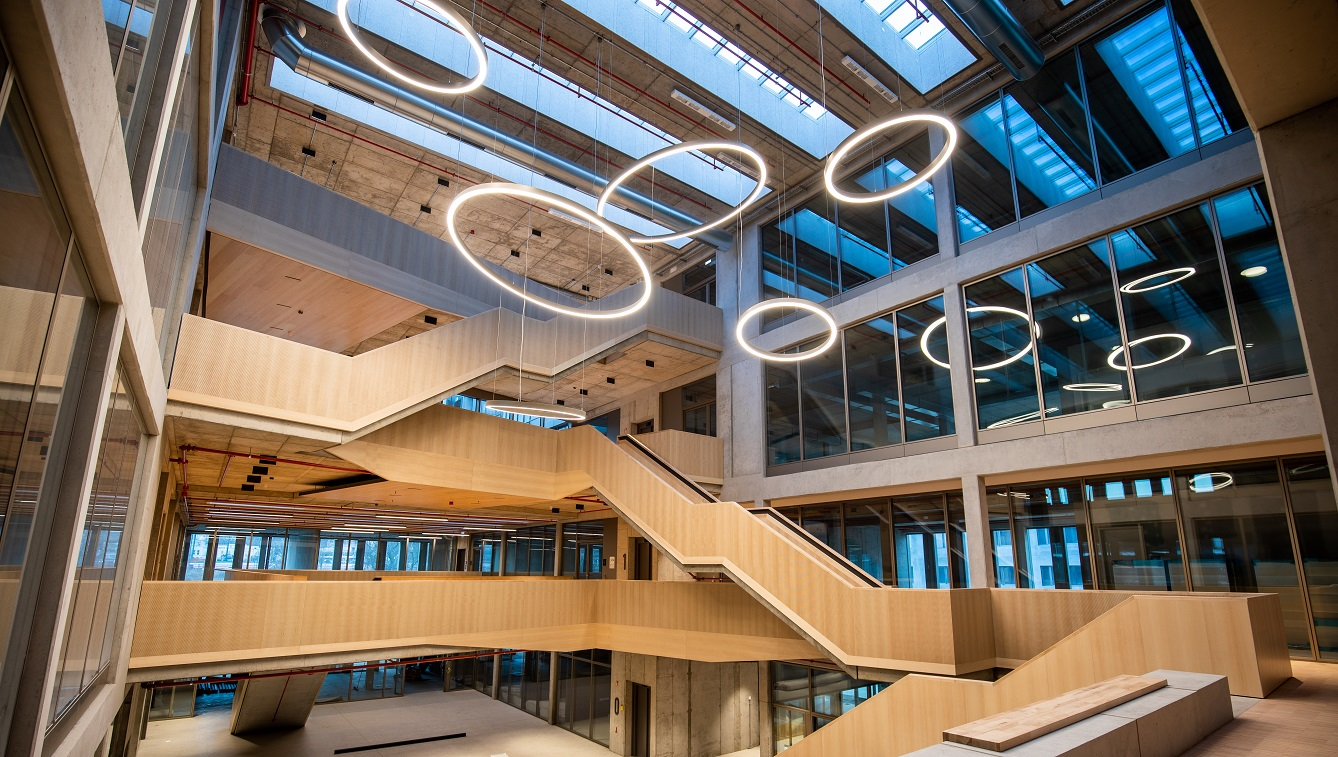
\includegraphics[width=\paperwidth, height=\paperheight, keepaspectratio]{attachments/campus}
            };
        \end{tikzpicture}
        
\includegraphics[width=0.6\textwidth]{attachments/logo}\par
        {\scshape\LARGE\bf Gisma University of Applied Sciences \par}
        {\scshape\Large\bf Department of Computer and Data Sciences \par}
        \vspace{1cm}
        \rule{\linewidth}{0.5mm}\par
        {\huge\bfseries\dissertationtitle\par} 
        \rule{\linewidth}{0.5mm}\par
        \vspace{0.2cm}
        {\Large\bf\student\par}
        \vspace{2cm}
        {\large Submitted in partial fulfillment of the requirements for the degree of\par}
        {\Large\bf\degree\par}
        \vspace{1cm}
        {\large Under supervision of\par}
        {\large\bf\supervisor\par}
        \vspace{0.5cm}
        {\large\submissiontime\par}
    }
    % \newpage  % Add this to ensure the next page starts fresh
    \pagestyle{fancy}  % Reset page style to fancy for subsequent pages
}

% Begin document
\begin{document}

\maketitle

% Abstract
\chapter*{Abstract}
\addcontentsline{toc}{chapter}{Abstract}

In this research paper, an robust, effective and efficient deep learning model is developed. And aims to improve the intepretablity of predictions for clinical applications. This paper included the devel and assessment of a deep learning model for the categorization of Alzheimer's disease stages using MRI images. Building on a well performing Kaggle model, the model adds many improvements, such as the ability to estimate uncertainty to produce prediction confidence scores. These confidence scores help doctors or clinicians to make well-informed decisions by offering insightful information about the model's decision-making process. The algorithm successfully classifies MRI pictures into the four stages of Alzheimer's disease that is Mild Demented, Moderate Demented, Non-Demented, and Very Mild Demented in achieving an accuracy of 99.55\% on the test dataset which was a slight improvement over the base model. By measuring prediction uncertainty estimation using Monte Carlo Dropout improves the model's robustness. This helps the clinicians to get the idea about the confidence of the model
Even though introduction of uncertainty estimation leads to longer prediction time, the suggested model shows improvement in training and assessment times when compared to the base Kaggle model. The model's better performance and ability to provide confidence scores makes up for the extra calculation expenses. A web application has been developed to increase the model's accessibility even further. Users can input MRI pictures to receive predictions and confidence scores. This intuitive interface allows simple integration into clinical settings, helping doctors in efficiently evaluating the model's results. The findings show how integrating uncertainty-aware deep learning models into medical diagnostics will improve Alzheimer's disease patient care, clinical desicion making, and early detection.

\vfill
\chapter*{Acknowledgements}
I sincerely thank Prof. Dr. Mazhar Hameed for all of his guidance and encouragement during the writing process of my thesis. His knowledge in machine learning and his helpful criticism have greatly influenced the quality and trajectory of this work.
I want to express my gratitude to the faculty and staff at Gisma University of Applied Sciences for offering me the materials and space I needed to carry out my research. Their understanding and motivation have been crucial in helping me in accomplishing this goal.
I express utmost gratitude for my friends and peers who encouraged me along this journey by sharing their knowledge and providing unwavering support. Particularly in trying times, their assistance and companionship have been a source of strength.
I am truly and incredibly grateful to my family for their constant unconditional love, understanding, and patience. Their constant support for me and my goals has been a continual source of inspiration and has been essential in enabling me to overcome every challenge.
In the end, I extend my sincere gratitude and dedicate my work to everyone who have helped and motivated , directly or indirectly. The contribution has had an enormous influence on my academic and personal growth as well as to this thesis.
\begin{flushright}
    \textit{Jason Joel Pinto} \\
    \textit{21 December 2024}
\end{flushright}
\vfill


% Acknowledgments
% \chapter*{Acknowledgments}
% \addcontentsline{toc}{chapter}{Acknowledgments}
% Write your acknowledgments here.

% Table of contents
\tableofcontents
\listoffigures % Optional
\listoftables  % Optional

% Chapters
\chapter{Introductions}
\thispagestyle{fancy}

Alzheimer's is a neurological problem that starts with a build up of proteins called amyloid plaques and neurofibrillary tangles. This leads to the brain cells to die over time and this leads to the shrinkage of the brain size\cite{mayo_alzheimers_2024}. Studies show us that about 5.4 million people in the States have Alzheimer's. And the studies show upward trend in the newer generations in getting Alzheimer's Disease. It is expected to increase by 10 million people. As of today every 68 second and new person is being diagnosed by Alzheimer's Disease. And the studies show that by 2050 this is going to decrease to 33 seconds\cite{2012131}. Between the year 2000 and 2017 the deaths reported due to alzheimer's have been increased by 143 \%\cite{2019321}. Alzheimer's is a disease which get's worse over the years, it keeps on progressing and the worst thing it is not reversible. Once worsened a lot of time and efforts go into the alzheimer's diseace. Which might end up being one of the costliest disease for any countries economy\cite{10.3389/fnagi.2024.1363458}. Hence it becomes very important that it is diagnosed as a early stage so that it can be controlled and treated. If it is detected early then doctor's with the help of medications can make sure that brain damage is not worsened. Currently magnetic resonance imaging (MRI),functional magetic resonance imaging(fMRI), computer tomography and positron emission tomography (PET) are used in order to early detect the Alzheimer's disease. These technologies are very expensive, very time consuming task and not very accessible for everyone as it Requirement sophisticated machines.

Machine Learning can be used to find if there is a way where one can find if there is a way models can find patterns which makes it possible to detect the disease at even earlier stage. As there are various studies that are being conducted all around the world, there are various data that are available which can be used by the machine learning models to analyze and early detect the disease. Based on prior researches, the researchers have numerical data's related to a persons MRI's and biomarkers in a persons body. With help of these they find whether a person is demented or not. If these data are used and ML model be developed which will be able to predict the will be lead to inexpensive diagnosis and can be made easily available to more and more people.

\begin{figure}[h!]
    \centering
    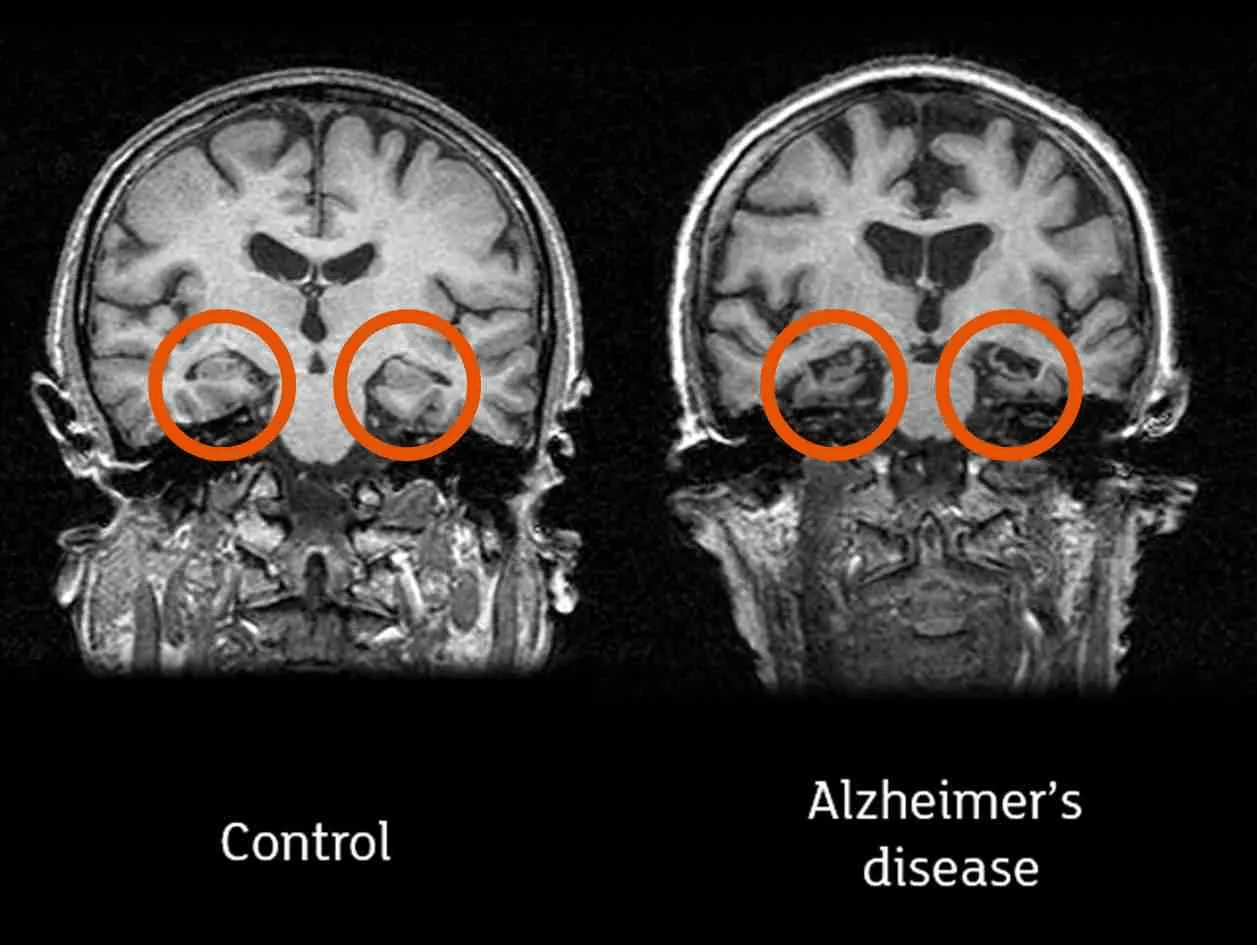
\includegraphics[width=0.8\columnwidth]{figures/fig1.png}  % Adjust the width to your liking
    \caption{Comparison of a normal brain (left) and an Alzheimer's patient's brain (right).\\Images credit: Professor John O'Brien, University of Cambridge and Newcastle University} % Caption for the image
    \label{fig:alzheimers_brain} % Label to reference the image later in the document
\end{figure}

A person with Alzheimer's disease will not be aware that he might be having a disease can ultimately lead to be a very dangerous disease. This is because the symptoms of Alzheimer's are very hard to find. It can be different to different people. The person can still do all the regular chores he does day to day without any problems. Having said that there will be some problems he might be facing while doing these activities, like for example not able to remember words, or not remembering names etc. People around him will definitely notice that this person has trouble remembering stuff. This is the reason why doctor as a first step usually conducts a medical interview where the person will be asked some questions. With the help of this he will be able to get a ball park idea whether he might have Alzheimer's or not. Some of the symptoms of Alzheimer's as follows,
\begin{enumerate}[nosep]
    \item Forgetting things, misplacing things, and missing meetings.
    \item Forgetting names and events.
    \item Not able to recall incidents happened in the past.
    \item Problems with audio visual memory.
    \item Being absent minded.
    \item Agitation and restlessness
\end{enumerate}

The symptoms of Alzheimer's becomes more evident when the disease progresses and one grows old. The person starts notices that the symptoms that he previously had are slowly slowly getting worse and worse. At later stages of AD it becomes very difficult to even communicate with the person as he does not remember anything. He forgets to even do the basic things that he has been taught to do since his childhood.

\chapter{Motivation}

\begin{figure}[h!]
    \centering
    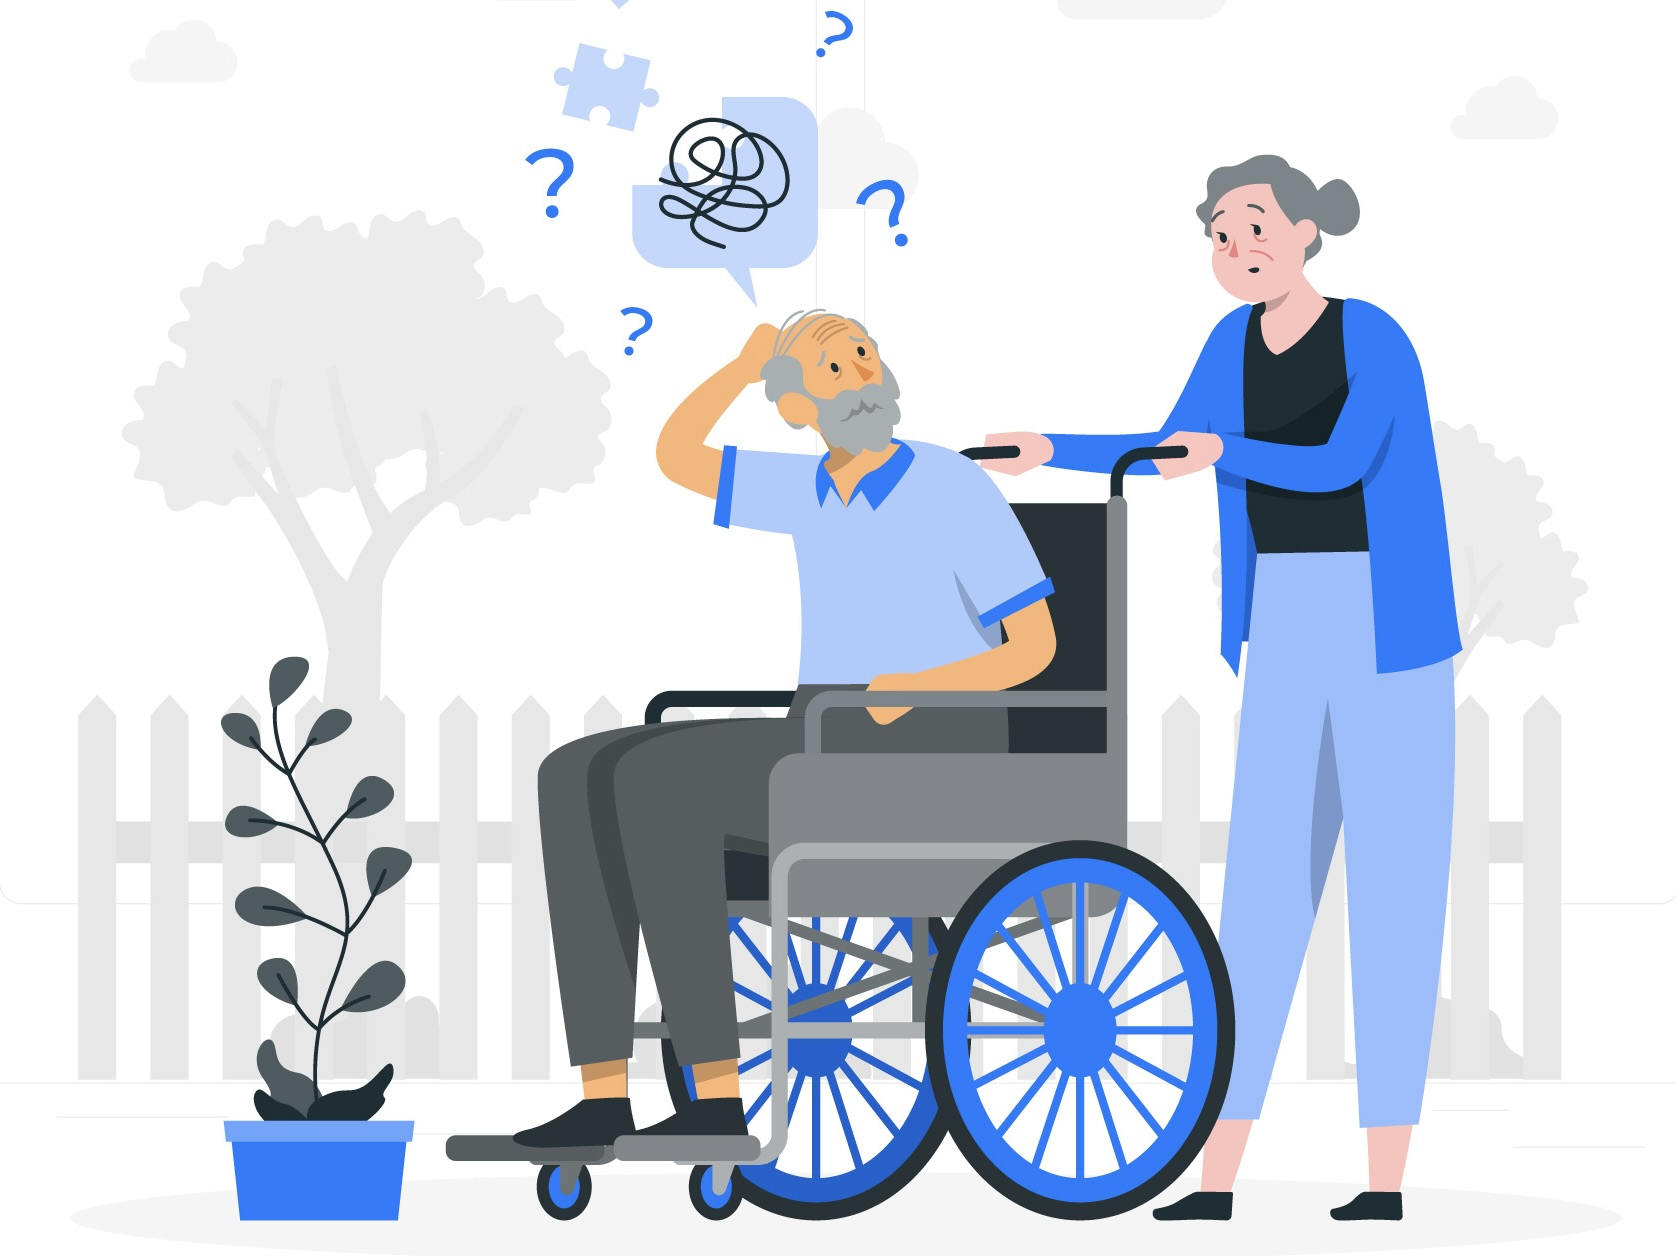
\includegraphics[width=0.8\columnwidth]{figures/fig2.jpeg}  % Adjust the width to your liking
    \caption{Person suffering from Dementia} % Caption for the image
    \label{fig:alzheimers_patient} % Label to reference the image later in the document
\end{figure}

Alzheimer's is considered as one of the most challenging disease in the modern medicine research. And this disease not only effects the individual but also impacts the people around him/her that is family, doctors and also the hospitals. As the people effected by this disease are increase at a rapid rate around us, there is a need to develop a better way to diagnose and prevent this disease. Particularly, there is a high demand for a system that will detect the disease at a early stage. So that the medical team can stop the disease from getting worse at the old age which might cause a big economic burger for the patients.

The motivation to write this thesis came from the fact that there are sophisticated diagnostics options available at the moment which are very expensive, time-consuming and they are not accessible for of people. But the main problem is even after spending a lot of money on these diagnostic procedures, it cannot detect it at a very earlier stage. Doctors use MRI's and PET scans which are very accurate but they machines used for this are very special and needs an expert to use them. Additionally, even after analyzing a persons brain in these scans, the disease is not detected at a early stage because the small changes that are happening in the brain are very different to find when compared to the normal aging of a persons brain. 

With the advanced Machine Learning techniques we can try to fix these problems that are currently there. By using the datasets that available online the advanced Machine Learning models can find patterns in the datasets which is hard to find using a naked human eyes. This will help in detecting the  Alzheimer's disease at a very earlier stage. 

Personally for me this paper is driven by the fact that I have seen many people around me struggling with Alzheimer's disease in their old age. I have seen it first hand how much time, money and effort does it take for their family to take care of them in that situation. As it is a disease that gradually gets worse, they slowly start losing their memory and identity. Having witnessed this I have seen how much effort goes into taking care of a Alzheimer's patient. This has motivated me to provide my Contribution to this communicate and make a difference. Hence, my aim in this research is to create a model will be able to predict the possibility of the disease at a earlier stage. 


\chapter{Contribution}

The contribution of this thesis paper is to use the advanced Machine Learning algorithms to find a solution to problems of early detection of the Alzheimer's disease. This is to provide a novel extension to the community of deep learning models to the Alzheimer’s stage classification.This will include implementing various different advance machine learning models to improve the predicting of the disease based on the MRI images that we are using for this research. The main contributions are such as:

\begin{enumerate}
    \item \textbf{ Inclusion of Uncertainty-Aware Framework:} In this research patient's MRI images will be analyzed which are divided into various stages of Alzheimer's and build a Classification Model using these images. Many high performing models are already presend online but in this thesis we will looking one of them and which performed the best and implement Monte Carlo Dropout Uncertainty calculation so that the confidence of the model can be analyzed.

    \item  \textbf{ Improved Model Interpretation:} The addition made to the code to include the Uncertainty indication will help in knowing how confident the model is when predicting the classes. This will also help in the clinical environment where the professionals looking at the results of the models they will not blindly accept the stage of alzheimer's disease, they can check if the model was confident when predicting the class. If not they can further review with their senior doctors about the case.

    \item \textbf{ Addition of Uncertainty Score in Predicted Results:}
    In this thesis a very much necessary steps in the deep learning models when it comes to medical usage are being looked at and included. These additional metrics will ensure that models performance is not evaluated only based on the accuracy but important factors like Uncertainty or confidence is considered so that cases with high uncertainty can be taken for further studies instead of just labeling whatever the model is classifying it as. A well structure visualization framework is put into action to highlight uncertainty for each and every individual predicted images. These information on the visualization will allow clinicians to find and focus on unique and unknown cases, which will allow them to make more informed decision-making.
    

    \item \textbf{Utilization of Publicly Available Datasets:} The MRI images used for this study is a cleaned dataset which is availabel on kaggle which is sourced from ADNI websites which are the MRI images of actual people with true labels. Since it's is very reliable source this study uses real world data to train the model at the same time following all the ethical guidelines.
    
    \item \textbf{Visualization of Uncertainty in Predictions:} By focusing on machine learning approaches, the research aims to provide scalable and cost-effective solutions for early AD diagnosis. This could significantly improve accessibility, especially in resource-constrained settings where sophisticated imaging technologies are not viable.

    \item \textbf{New addition will make it possible for this to be applied in a clinical setup:} By introduction Uncertainty into account when classifying the Alzheimer’s Disease into multiple classes this thesis reseach will help reducing the rist of wrong diagnosis in a medical setup who are ready to introduce AI into for their diagnostics setup. It is especially important in medical field as misdiagnosis might cause a major problems in a persons life.

    \item \textbf{Contribution to the AD community as well as open sourcing these projects:} The code used for this thesis will be open to everyone to view and as this will allow to access and reproduce this models for further studies. By adding Uncertainty to these already well performing models this reasearch further improves the the communities acceptence of these new technologies into their system, as it also allows human proffessionals to take things into their hands the models is not so sure how to react the unexpected situations.

\end{enumerate}



\chapter{Literature Review}

In the recent years have seen a impressive amount of progress in the utilization of the deep learning models for the Alzheimer’s Disease detection based on the MRI data. And alot of advancement focus on how to improve, how accurately the model predicts the Disease of how accurately it classifies the images or data into different classes. Whereas the integration of Uncertainty calculation is something that is not explored too much, nevertheless. In this Literature review the previous research papers are being studied and will be compared and seen if there are any gaps in the study that can be full filled.

\section{Overview of techniques used on MRI}
All thanks to the impressive technology of the Magnetic Resonance Imaging(MRI), Alzheimer's disease (AD) can be detected at a very early stage compared to earlier. The 3 Dimensional high quality images of brain captured using MRI machines provide a view of our brain with which we can find the patterns in the parts of the brain like temporal regions and hippocampal region which helps in diagnose of the Alzheimer’s Disease. By taking a look at the white matter integrity and functional connectivity, the help of diffusion tensor imaging (DTI) and functional magnetic resonance imaging (fMRI) make amazing contributions to this. Methods such as cortical thickness measurement and voxel-based morphometry have been widely used for quantitative analysis of structural changes and brain volume\cite{zou2023}.

Recently, there have been studies that are going on to create synthetic longitudinal MRI images for Alzheimer's disease using a conditional diffusion model. Diffusion models are are excellent at producing high-quality images with consistent training, which are used in this strategy. The models can produce realistic target pictures that mimic the course of the disease by using the time interval and the source MRI scan as conditioning elements. This strategy may be able to get around the drawbacks of current techniques like GANs and VAEs, which can have unstable, undiversified, or hazy results. The suggested model offers a useful tool for Alzheimer's disease research and clinical applications, producing high-fidelity synthetic MRI scans with encouraging findings\cite{Duy2024}.


\section{Using Deep Learning for Alzheimer’s Detection}
The most common type of dementia that causes a lot of trouble for  millions of people worldwide is Alzheimer's disease (AD). In order to manage symptoms and maybe reduce the progression of the disease, early recognition of AD is essential\cite{2023ShenLiu}.Conventional diagnosis techniques depend on radiologists' subjective and time-consuming manual review of brain imaging data. And that is where Deep Learning brings an serious advantage over the time consuming tasks.

With the use of deep neural networds we have see an amazing results in the recent years. Using the MRI data, and deep learning neural networks in prediction of the early detection of the Alzheimer’s Disease has been a very promision method with great acccuracy. The convolutional neural networks as well as the recurrent neural netword have have drastically improve the prediction for this desease when compared to the traditionaL Machine Learning alternatives. This is because the Deep Learning models are able undertand the complex nature of the high dementional data that are used in training these models and to capture the brain image\cite{2019Jo}. Recent improvements in the this field, specially deep leaning have changed the landscape of the Alzheimer’s Detection. It is able to provide an objective and efficient solution.

Convolutional Neural Networks (CNNs) is a kind of deep learning model which has showed the world it's abilities with great results in prediction of Alzheimer’s with the help of MRI images. Very high resolution images or high dimensional data's can be trained using these models, which will find the existing patters in these data, and helps in detecting Alzheimer’s at a very early stage. By drastically reducing the time and efforts required in the diagnosis process of the Alzheimer’s Disease and being able to predict with great precision,these deep learning models perform impressively better than than the conventional machine learning models.


Let's check some of the recent studies. The summary of the studies is provided in the Table~\ref{tab:methods_comparison} :
\begin{table*}[h!]
    \centering
    \caption{Comparison of Studies on Alzheimer’s Disease Detection}
    \label{tab:methods_comparison}
    \begin{tabular}{|p{3cm}|p{3cm}|p{3cm}|p{2cm}|p{4cm}|}
        \hline
        \textbf{Study} & \textbf{Dataset} & \textbf{Model} & \textbf{Accuracy} & \textbf{Limitations} \\ \hline
        Sharma, Sarang (2022) \cite{2022Sarang} & Kaggle & Hybrid Deep Learning Model & 91.75\% & No uncertainty estimation, limited interpretability \\ \hline
        Desai, Maitri (2024) \cite{2024Desai} & OASIS & Multi-Task CNN & 91.0\% & Limited generalizability, lacks uncertainty \\ \hline
        Ahmed, Gulnaz (2022) \cite{2022Ahmed} & OASIS & DAD-Net & 99.22\% & No reliability or uncertainty analysis \\ \hline
        Sarraf et al. (2016) \cite{sarraf2016} & ADNI & CNN (LeNet-5) & 98.84\% & High false negatives \\ \hline
        Farhana Islam et al. (2023) \cite{Islam2023} & Custom MRI Dataset & ResNet-50 & 98.71\% & No uncertainty estimation \\ \hline
        Santos et al. (2023)  \cite{Santos2023} & Kaggle & Neural Network & 80.6\% & Moderate accuracy, lacks optimization \\ \hline
        El-Latif et al. (2023) \cite{Latif2023} & Kaggle & Lightweight Deep Learning Model & 95.9\% & No uncertainty quantification \\ \hline
        Isunuri et al. (2023) \cite{Isunuri2023} & Kaggle & Transfer Learning with CNN & 97.32\% & Limited interpretability \\ \hline
        Murugan et al. (2023) \cite{Murugan2021} & Kaggle & DEMNET & 95.23\% & No uncertainty assessment \\ \hline
        Gupta et al. (2023) \cite{Gupta2019} & NRC Korea & DEMNET & 96.89\% & No reliability metrics \\ \hline
        Mohammad. (2024) \cite{gobara_kaggle_notebook2024} & Kaggle & Xception & 99.6\% & No uncertainty calculation \\ \hline
    \end{tabular}
\end{table*}

In recent studies, various different techniques have been used to predict the alzheimers disease. Out of all of them deep learning models have shows a lot of potential and promise with great results. Deep learning is widely used acrross various fields or study, but the stream where we excel the most is classification of the images. As in recent times people are able to get hands on the powerful hardware as it has become accessible, and more research are being conducted on Deep Learning models there has been alot of improvement in the performance and hence the reliability of these models have been increased \cite{Yu2023}.
Particularly for alzheimer's there have been several studied that have been conducted. In this study we will be looking at few of them. In a paper by Sharma et al. \cite{2022Sarang} they propose HTLML. It is a hybrid deep learning model that uses the Kaggle dataset to predict the Alzheimer’s Disease. In their implementations they were able to achieve an accuracy of 91.75\%. Which is a very good performace. But what it lacks is the implementation of uncertainty estimation. When it comes to a clinical environment it would be very advantageous for clinicians to know how confident the model is. The lack of uncertainty estimation is a rather common gap found in many existing studies, limiting them to consider for a clinical deployment.In the reseach conducted by Desai et al. \cite{2024Desai}, they use a Multi-Task CNN model using the OASIS dataset to diagnose Alzheimer’s. Their model achieved an accuracy of 91.0\%, but limitations of the model is it's generalizability. The authors themselves mention in the paper that the model performs good on the OSIS dataset but it might struggle to perform well in the real-world clinical data. Generalizability is considered to be a very common issue with the deep learning models. Specially when there is not enough data to be trained on or there is no diverse patient data. Or when tested to perform with the real world data. In a paper by author Ahmed et al. \cite{2022Ahmed} has experimented with DAD-Net, it is also a deep learning-based model for Alzheimer’s detection. Here they have used ADASYN to oversample the data as the dataset they used was imbalanced. Using the deep leaning network they managed to get an impressive accuracy of 99.22\%. This model again however does not incorporate Uncertainty calcucation. Even through the model prediction is high, without the model confidence/ Uncertainty implementation it's implementation in a clinical environment will be very low because even when the model is struggling the clinicians needs to know it so that they can take a informed desicion. the model does not incorporate uncertainty estimation, which is a crucial factor for clinical decision-making. While the high accuracy is promising, the lack of uncertainty estimation limits the model's applicability in high-stakes environments such as healthcare.
Sarraf et al. \cite{sarraf2016} use CNNs and LeNet-5 for the classification of Alzheimer’s classification with the ADNI image dataset. They achieved an accuracy of 98.84\%. However, the study is criticized for its high false-negative rate, which can lead to misdiagnosis in clinical applications. Additionally, this work does not include any discussion of uncertainty estimation, further limiting its clinical relevance. Islam et al. \cite{Islam2023} proposed a method using the ResNet50 feature extractor and an SVM classifier for diagnosing Alzheimer’s disease from MRI images. This study achieved an accuracy of 98.71\%, but it lacked assessment of the model reliability. Since there is no assessment with the unseen data the reliablity of the model is hard to know with the real world data. Even in this paper the Uncertainty calcucation is not considered. Further in the study of neural network model for Alzheimer’s prediction by Santos et al. \cite{Santos2023}, they employed a neural network model on  the Kaggle dataset, and were able to get a accuracy of 80.6\%. While the model is able to provide the diagnosis and classification the performance of the model could be improved compared to other models. In the conclusion the authors suggested that the model could be improved through further research, but uncertainty estimation is not part of their investigation, which is a limitation. El-Latif et al. \cite{Latif2023} presented a very lightweight deep learning model for Alzheimer’s disease detection using MRI data. The model achieved an accuracy of 95.9\%, but like the previous case the authors acknowledged that the performance could be improved further. Again the lack of uncertainty estimation is a limitation. Isunuri et al. \cite{Isunuri2023} employ transfer learning and a CNN for Alzheimer’s severity classification, achieving an accuracy of 97.32\%. Even though the model demonstrates very good performance performance, there is no mention of uncertainty estimation, which could add a layer of reliability and interpretability to the model’s predictions. The authors also note that the model outperforms competing models in several metrics, yet its generalizability to other datasets is unclear.
Murugan et al. \cite{Murugan2021} introduced DEMNET, again it a type of deep learning model itself for the sake of early diagnosis of Alzheimer’s disease from MRI images. The model achieved an accuracy of 95.23\%, but the authors acknowledged that the performance of the model could have been be improved. While the model is promising, it does not incorporate uncertainty estimation, which is a critical aspect for clinical use as earlier mentioned where decisions based on model predictions can have serious consequences. Gupta et al. \cite{Gupta2019} use combined features from voxel-based morphometry and cortical, subcortical, and hippocampus regions of MRI T1 brain images for early Alzheimer’s diagnosis. With an accuracy of 96.89\%, the study demonstrates a robust method for Alzheimer’s detection. But similar to other studies, it lacks a mechanism for assessing uncertainty, which is important for practical deployment in healthcare environments. One of the model which particularly caught my attention was a kaggle model where where Mohammad \cite{gobara_kaggle_notebook2024} with the kaggle dataset was able to achieve a accuracy of 99.5\%. I will be selecting this model as my based model. The reason why I am selecting this model is because it was able to achieve this high accuracy score, even though the model was not have a complex architecture. This make the model very efficient and easy to deploy and maintain as a final product. But having said that there were some limitations in these model.

\section{Limitations of Existing Approaches}
Table \ref{tab:methods_comparison} all the previous existing papers and research have been summarized, it also highlights the study's limitations. Many papers and research have models that do exceptionally well with accuracy, but then all the paper lacks the attempt to include uncertainty score as an output which might turn out to be invaluable and crucial in a clinical environment in decision-making. Furthermore, some of the models had issues with high false-negative rates, less generalizability, and dataset bias still exists. These problems support a requirement or necessity for the inclusion of uncertainty estimation so that the clinical usability and reliability of the model can be improved. When the stakes are high in clinical settings, it is challenging to trust models that lack uncertainty measurements. Adding uncertainty estimates to deep learning models can improve their interoperability and give medical professionals important information about the accuracy of the model's predictions. By using uncertainty-aware deep learning to enhance the applicability of Alzheimer's diagnosis models, this study fills a significant gap in the body of existing literature.


\section{Novelty of the Proposed Approach}
The integration of uncertainty estimation into deep learning models addresses critical gaps in existing research. By providing confidence scores alongside predictions, clinicians can make informed decisions, reducing the risks associated with false negatives or overfitting to biased datasets. This approach also enhances model interoperability, a vital factor for clinical adoption.

\chapter{Methodology}

In this chapter the methodology used in this thesis for training, developing, evaluating and developing an uncertainty-aware deep learning model will be discussed. This sections will be taking you into the deep dive into why certain things are chosen over others. Each and every step from the loading of the dataset, data augmentation, model building, evaluation metrics, uncertainty awareness in the model and as well building an web application to predict Alzheimer's which can be used in a clinical environment.

\section{Dataset used for this research}

\subsection{About Dataset}

\begin{figure}[h!]
    \centering
    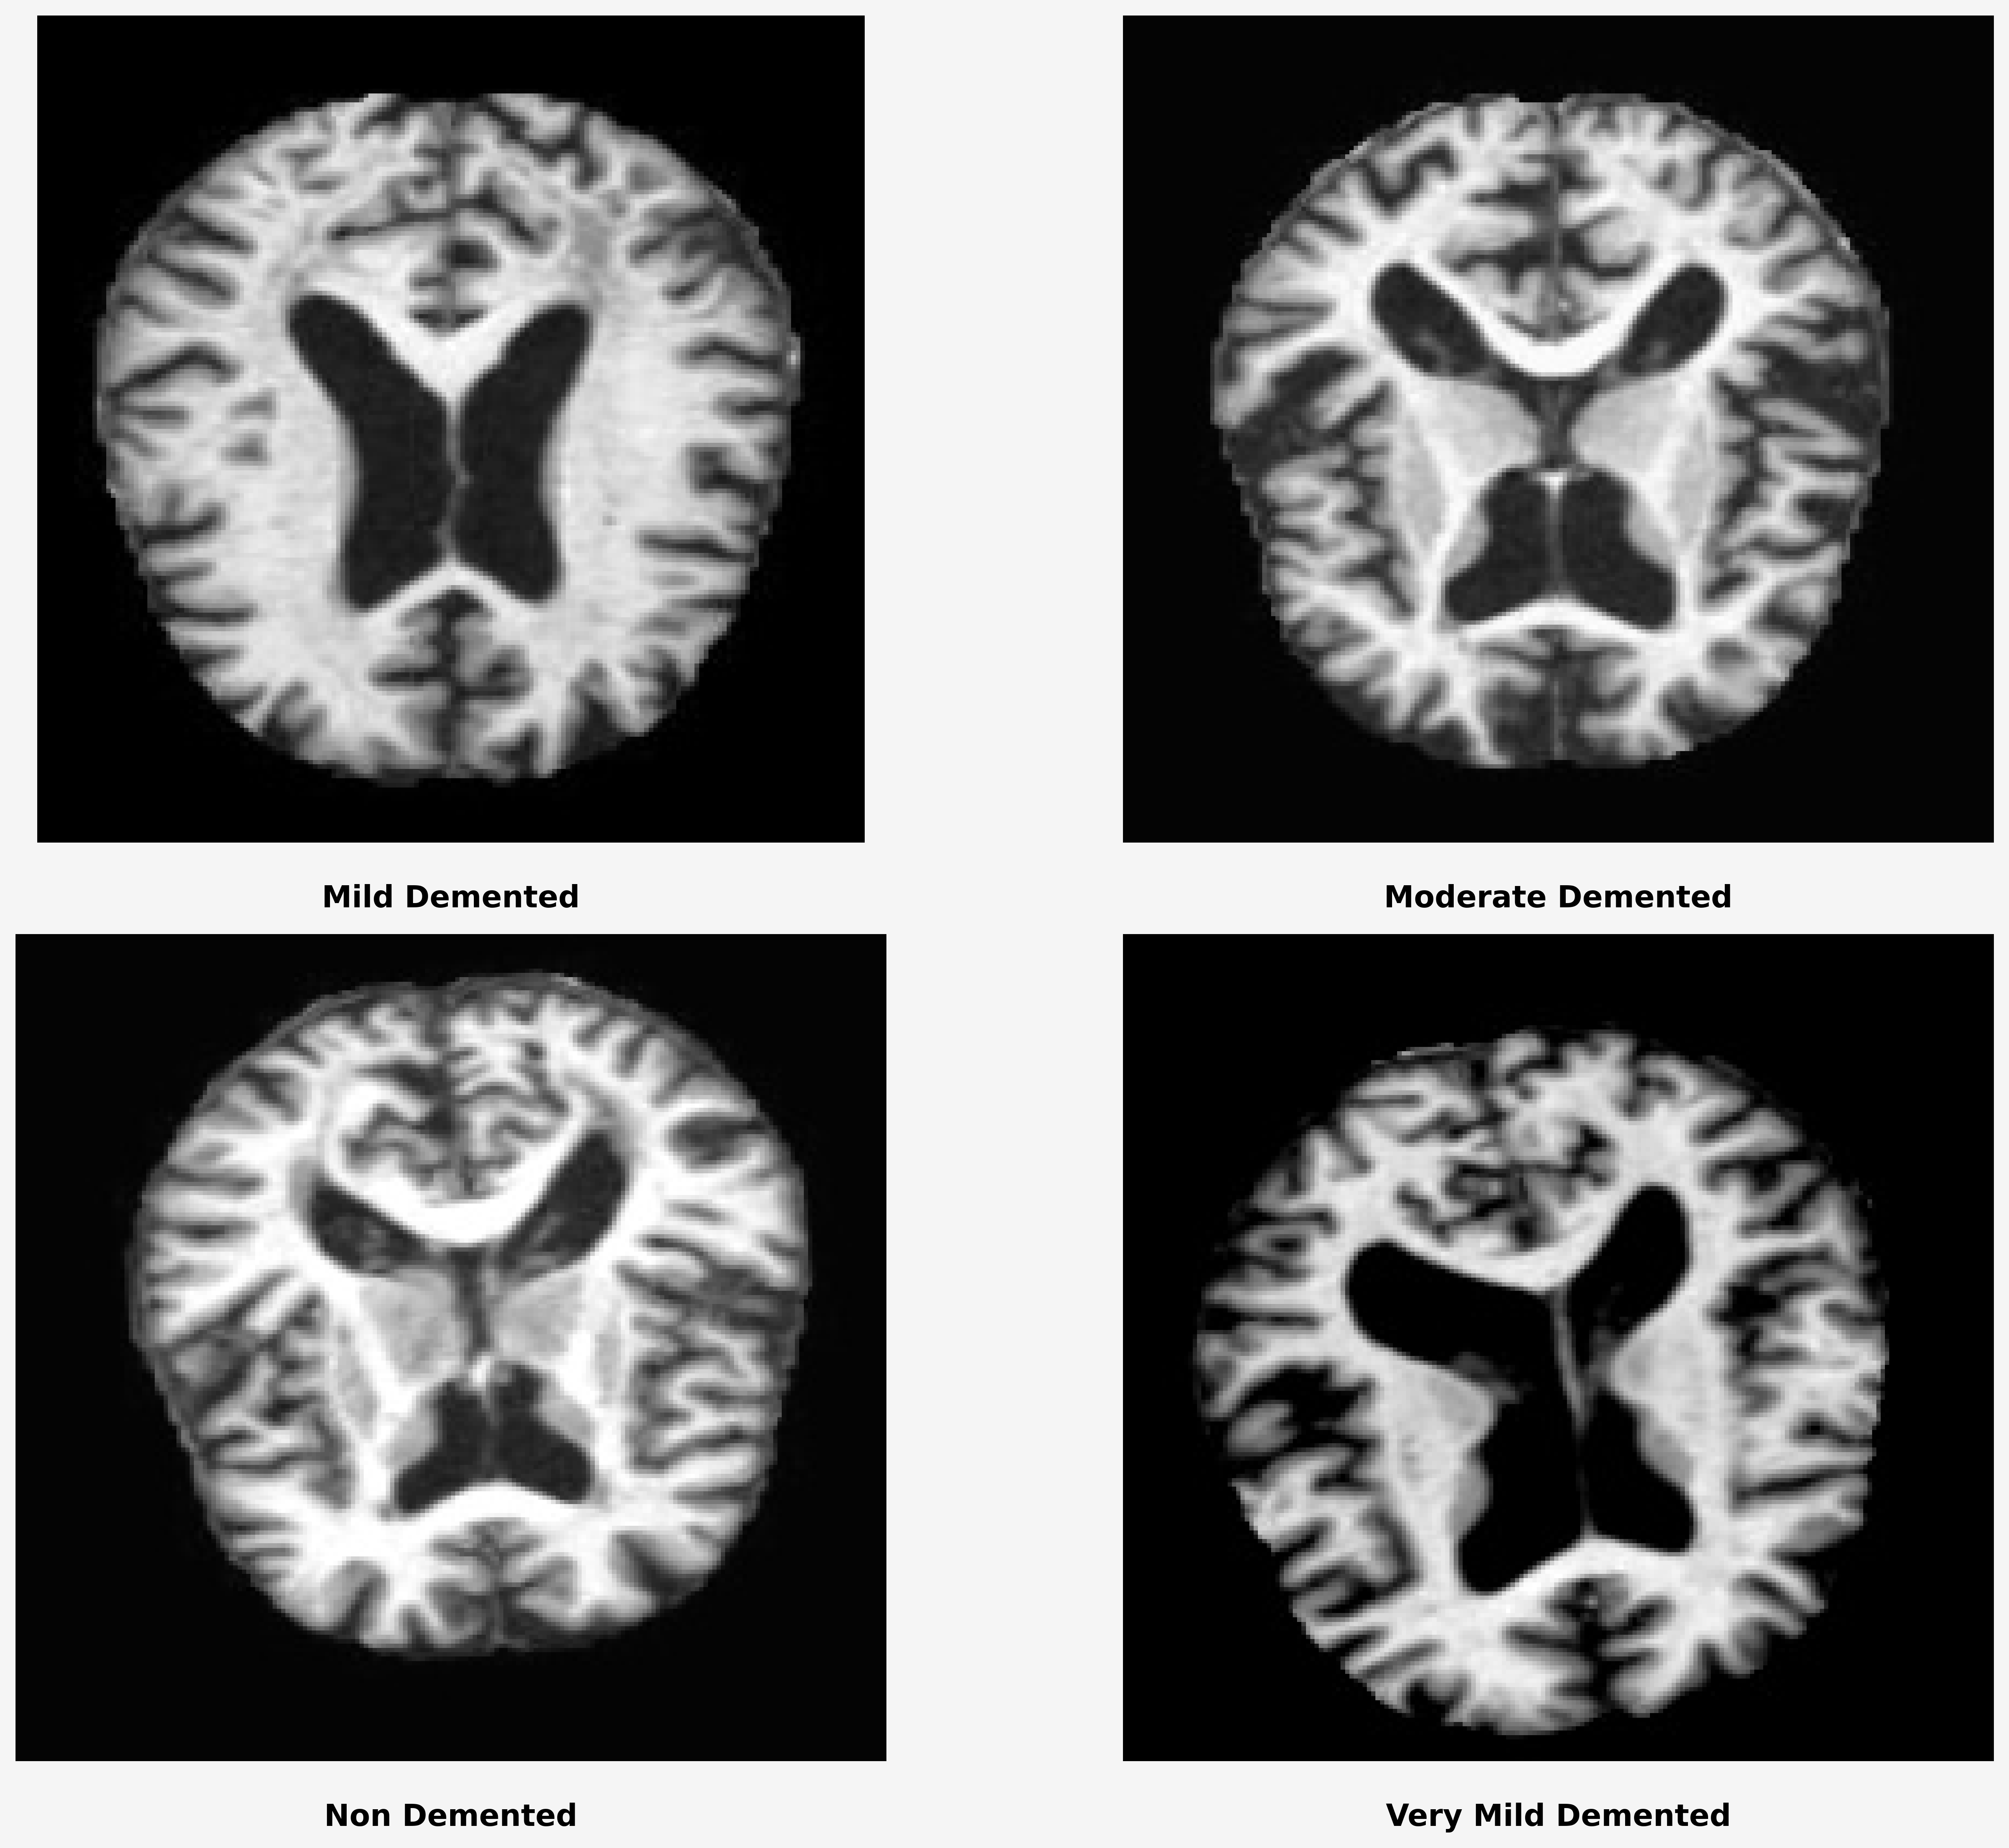
\includegraphics[width=0.8\columnwidth]{figures/dataset.png}  % Adjust the width to your liking
    \caption{Sample images of the dataset} % Caption for the image
    \label{fig:dataset} % Label to reference the image later in the document
\end{figure}

For this study the dataset used from a publicly available dataset. The dataset is available here \url{https://www.kaggle.com/datasets/uraninjo/augmented-alzheimer-mri-dataset}. This dataset is derived from the MRI dataset that is available on the ADNI website \url{https://adni.loni.usc.edu/}. This dataset consists of high quality 2D Magnetic Resonance imaging(MRI) scans images. Magnetic Resonance imaging scans are usually 3D, but this particular images dataset that is available on Kaggle is being processed and converted into high quality 2D images. This dataset is best suited for multi class classification task. The images are being divided into 4 different classes based on the stages of the alzheimer's the patients are in. And the folder names are the true labels of the images:
\begin{enumerate}
    \item \textbf{NonDemented} – This consist of MRI images of brains which does not show any sign of having Alzheimer’s Disease or in other words cognitive impairment. There are a total of 9600 images of the Non Demeted brains in this dataset.
    \item \textbf{VeryMildDemented} – This consists of MRI images of the brains which shows slight early sign's of patient progressing towards Alzheimer’s Disease. There are a total of 8960 images of the Very Mild Demented brains in this dataset.
    \item \textbf{MildDemented} – This consists of MRI images of the brains which show mild structural brain changes of patient progressing towards Alzheimer’s Disease. These patients will start having noticeable memory problems and cognitive problems. There are a total of 8960 images of the Mild Demented brains in this dataset.
    \item \textbf{ModerateDemented} – This consists of MRI images of the brains which shows significant structural brain changes of patient Alzheimer’s Disease. This is a advanced stage of the Alzheimer’s disease. These patients will start having noticeable memory problems and cognitive problems as well. There are a total of 6464 images of the Mild Demented brains in this dataset.
\end{enumerate}


\subsection{Dataset Features}
Let's look at the features of the dataset that is used for this paper. There are two set's of images data in this dataset. One is the original images and the second one is the augmented images. For this research we will be taking Augmented images as the base models that we are taking from the Kaggle source has used this dataset. Hence we will be using this. The images are divided into 4 classes and images of each classes are placed in their on Folder's namely, NonDemented, VeryMildDemented, MildDemented and ModerateDemented.
\begin{enumerate}
    \item \textbf{Size of Dataset} 
    – The total size of the dataset is 366 megabytes. It consists of thousands of high quality 2 dimensional images for each classes. Which makes this dataset a perfect fit for the building a machine learning models by training the model using these real world datasets.
    \item \textbf{Dimensions of the Dataset} – The original images of this datasets roots from the collection of MRI images from ADNI dataset. These images are originally 3 Dimensional. Having said that the dataset used for thesis are the processed images of the ADNI dataset. The images have been processed to convert to 2 Dimensional images. This helps to reduce the complexity of the model.
    \item \textbf{Class balance} 
    \begin{figure}[h!]
        \centering
        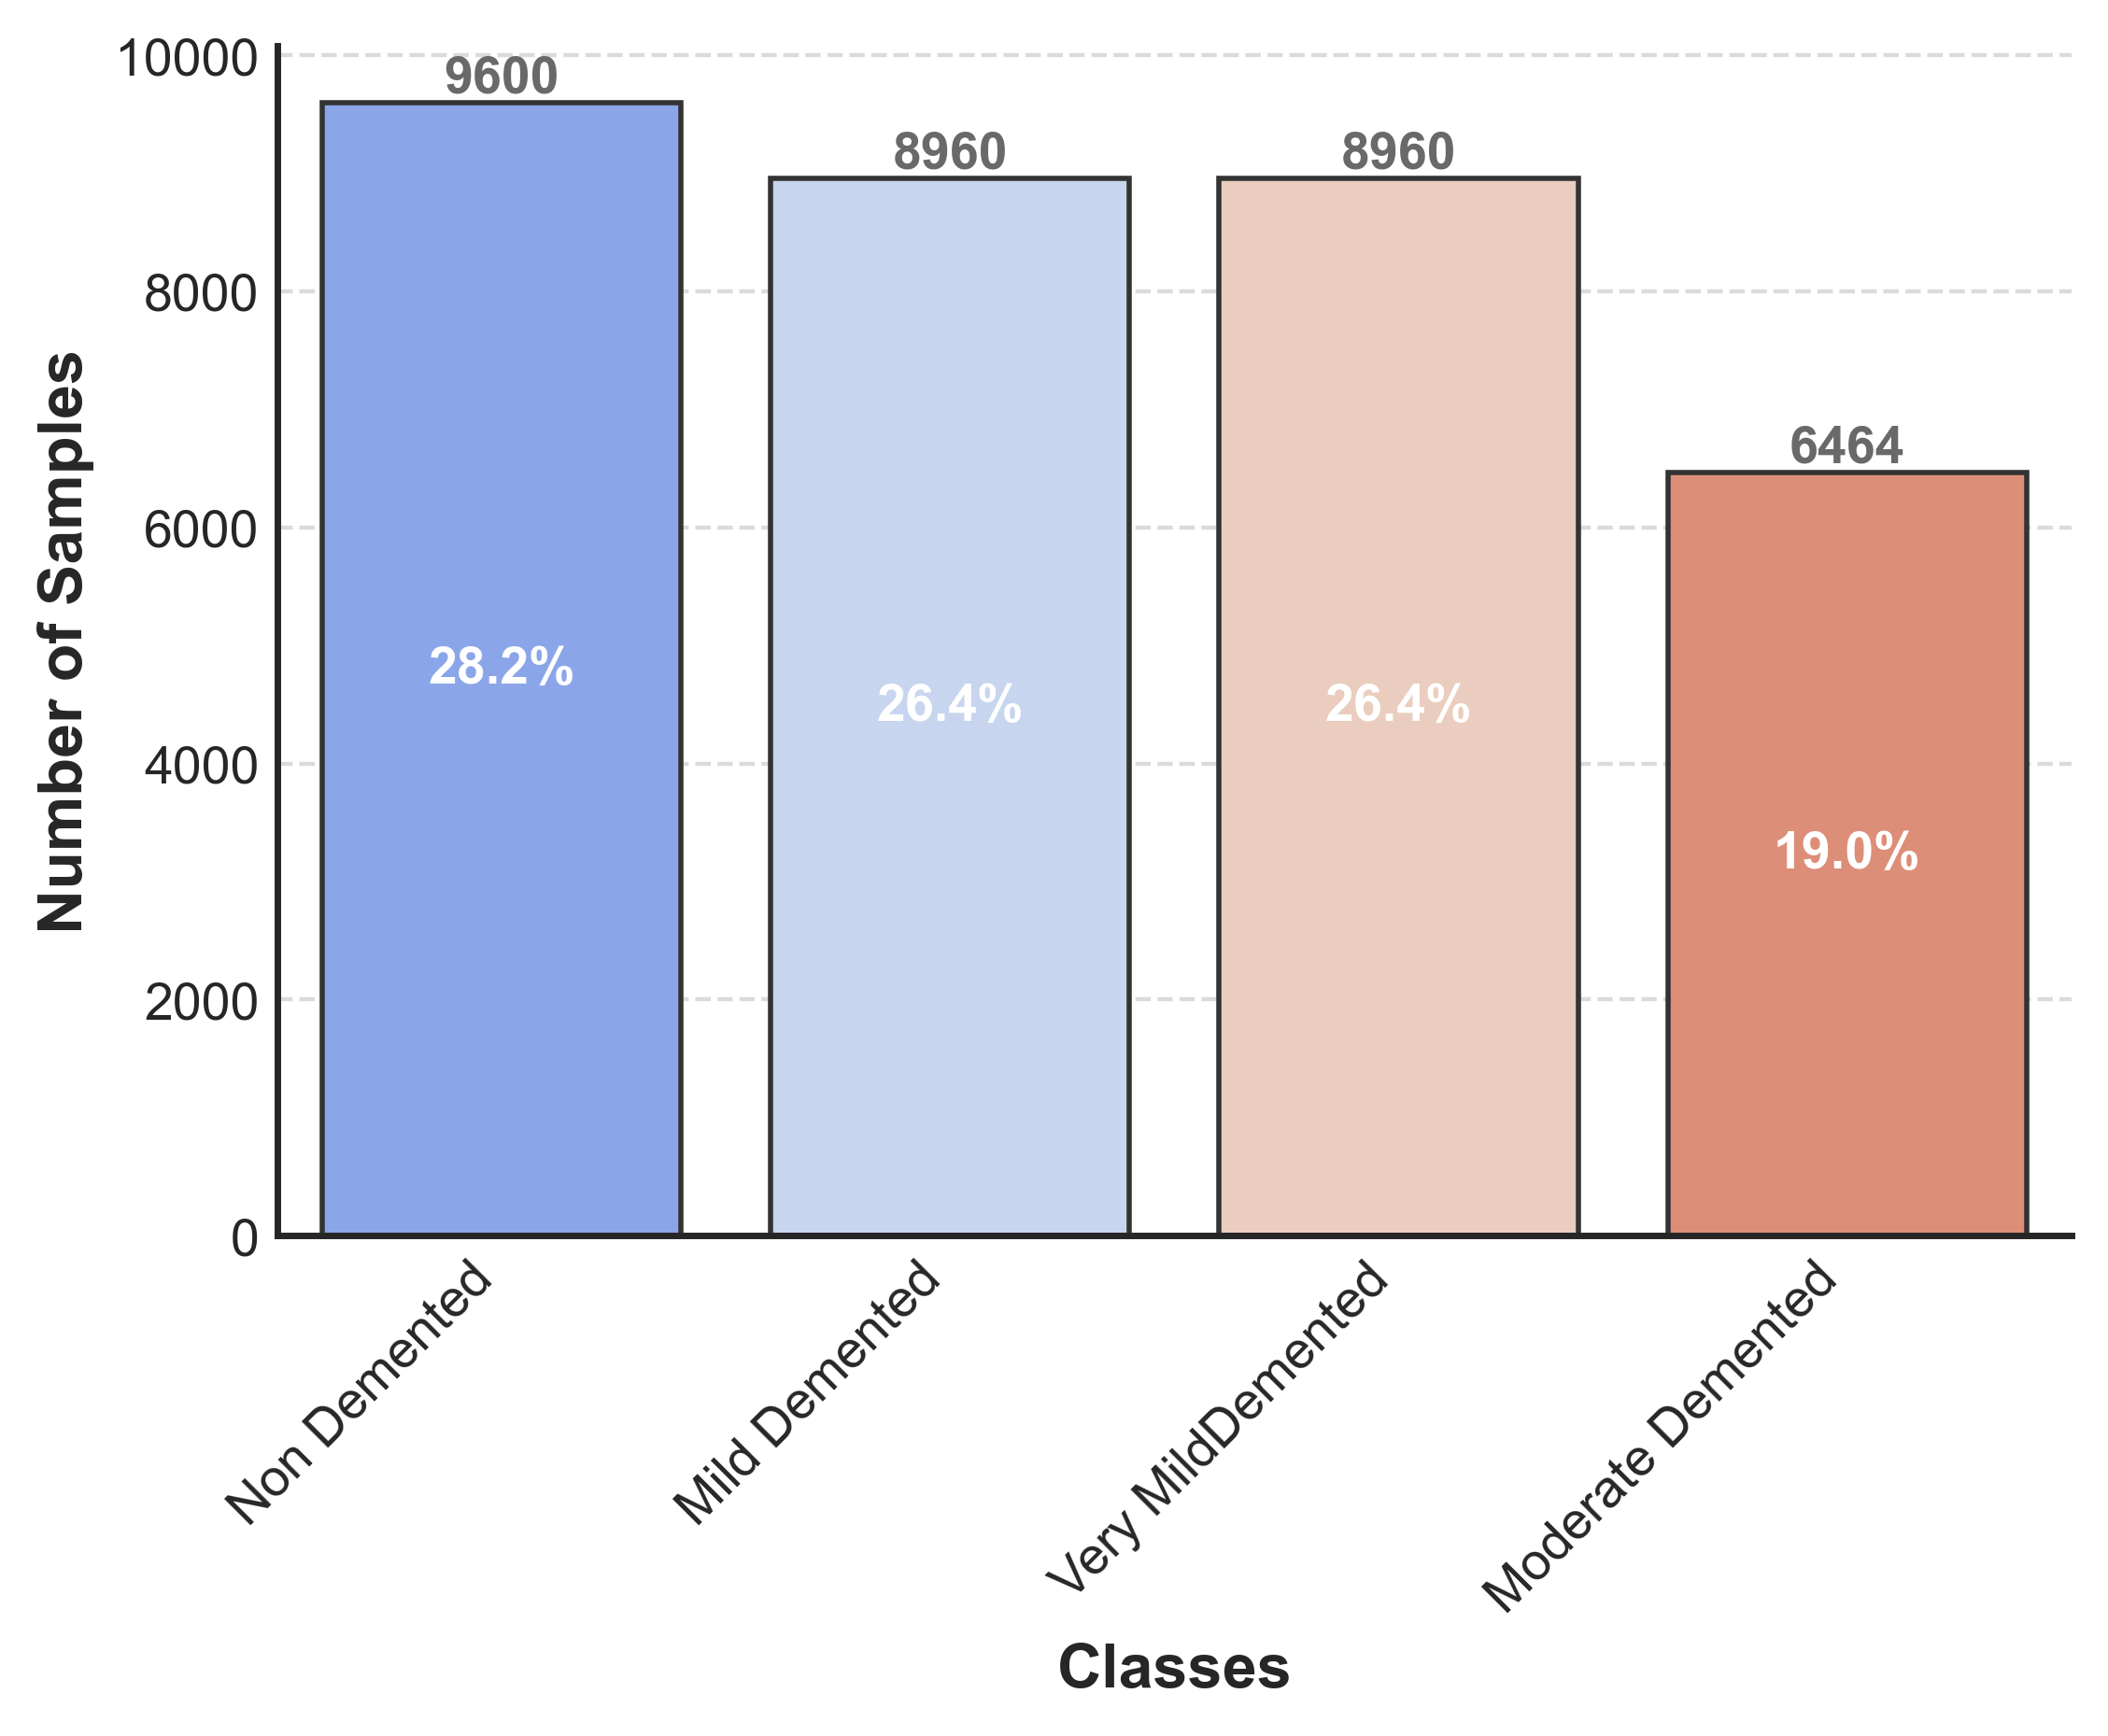
\includegraphics[width=0.8\columnwidth]{figures/dataset_class_distribution.png}  % Adjust the width to your liking
        \caption{Dataset Class distribution} % Caption for the image
        \label{fig:dataset_class_distribution} % Label to reference the image later in the document
    \end{figure}
    – The figure \ref{fig:dataset_class_distribution} shows the class distribution in the dataset. As you can see in the figure \ref{fig:dataset_class_distribution} there 9600 images for Non Demented Class, and 8960 images for Mild Demented and Very Mild Demented Class and 6464 images for Moderately Demented Class. It is a moderately imbalanced dataset. But since we are going to check for accuracy scores for each classes we are not going to balance this dataset.
    \item \textbf{Dataset Format} – Originally the ADNI datasets are stored in NIfTI format. But the Kaggle dataset that we are using is being preprocessed and saved in 2D format, all the images are stored in JPG format.
\end{enumerate}

\subsection{Ethical and Legal Considerations}
This research used a publicly available Kaggle dataset for Alzheimer’s disease detection, which strictly adheres to its licensing terms and conditions. The dataset used in this thesis is already anonymized by its authors which complies with data privacy and confidentiality standards by excluding personally identifiable information. Ethical considerations, including fairness, transparency, and interoperability, were of highest priority when designing the model. The use of Kaggle data aligns with non-commercial academic purposes, and proper attribution to the dataset’s creators is provided. No new data was collected for this study.

\section{Pre-Processing the Dataset}
\begin{figure}[h!]
    \centering
    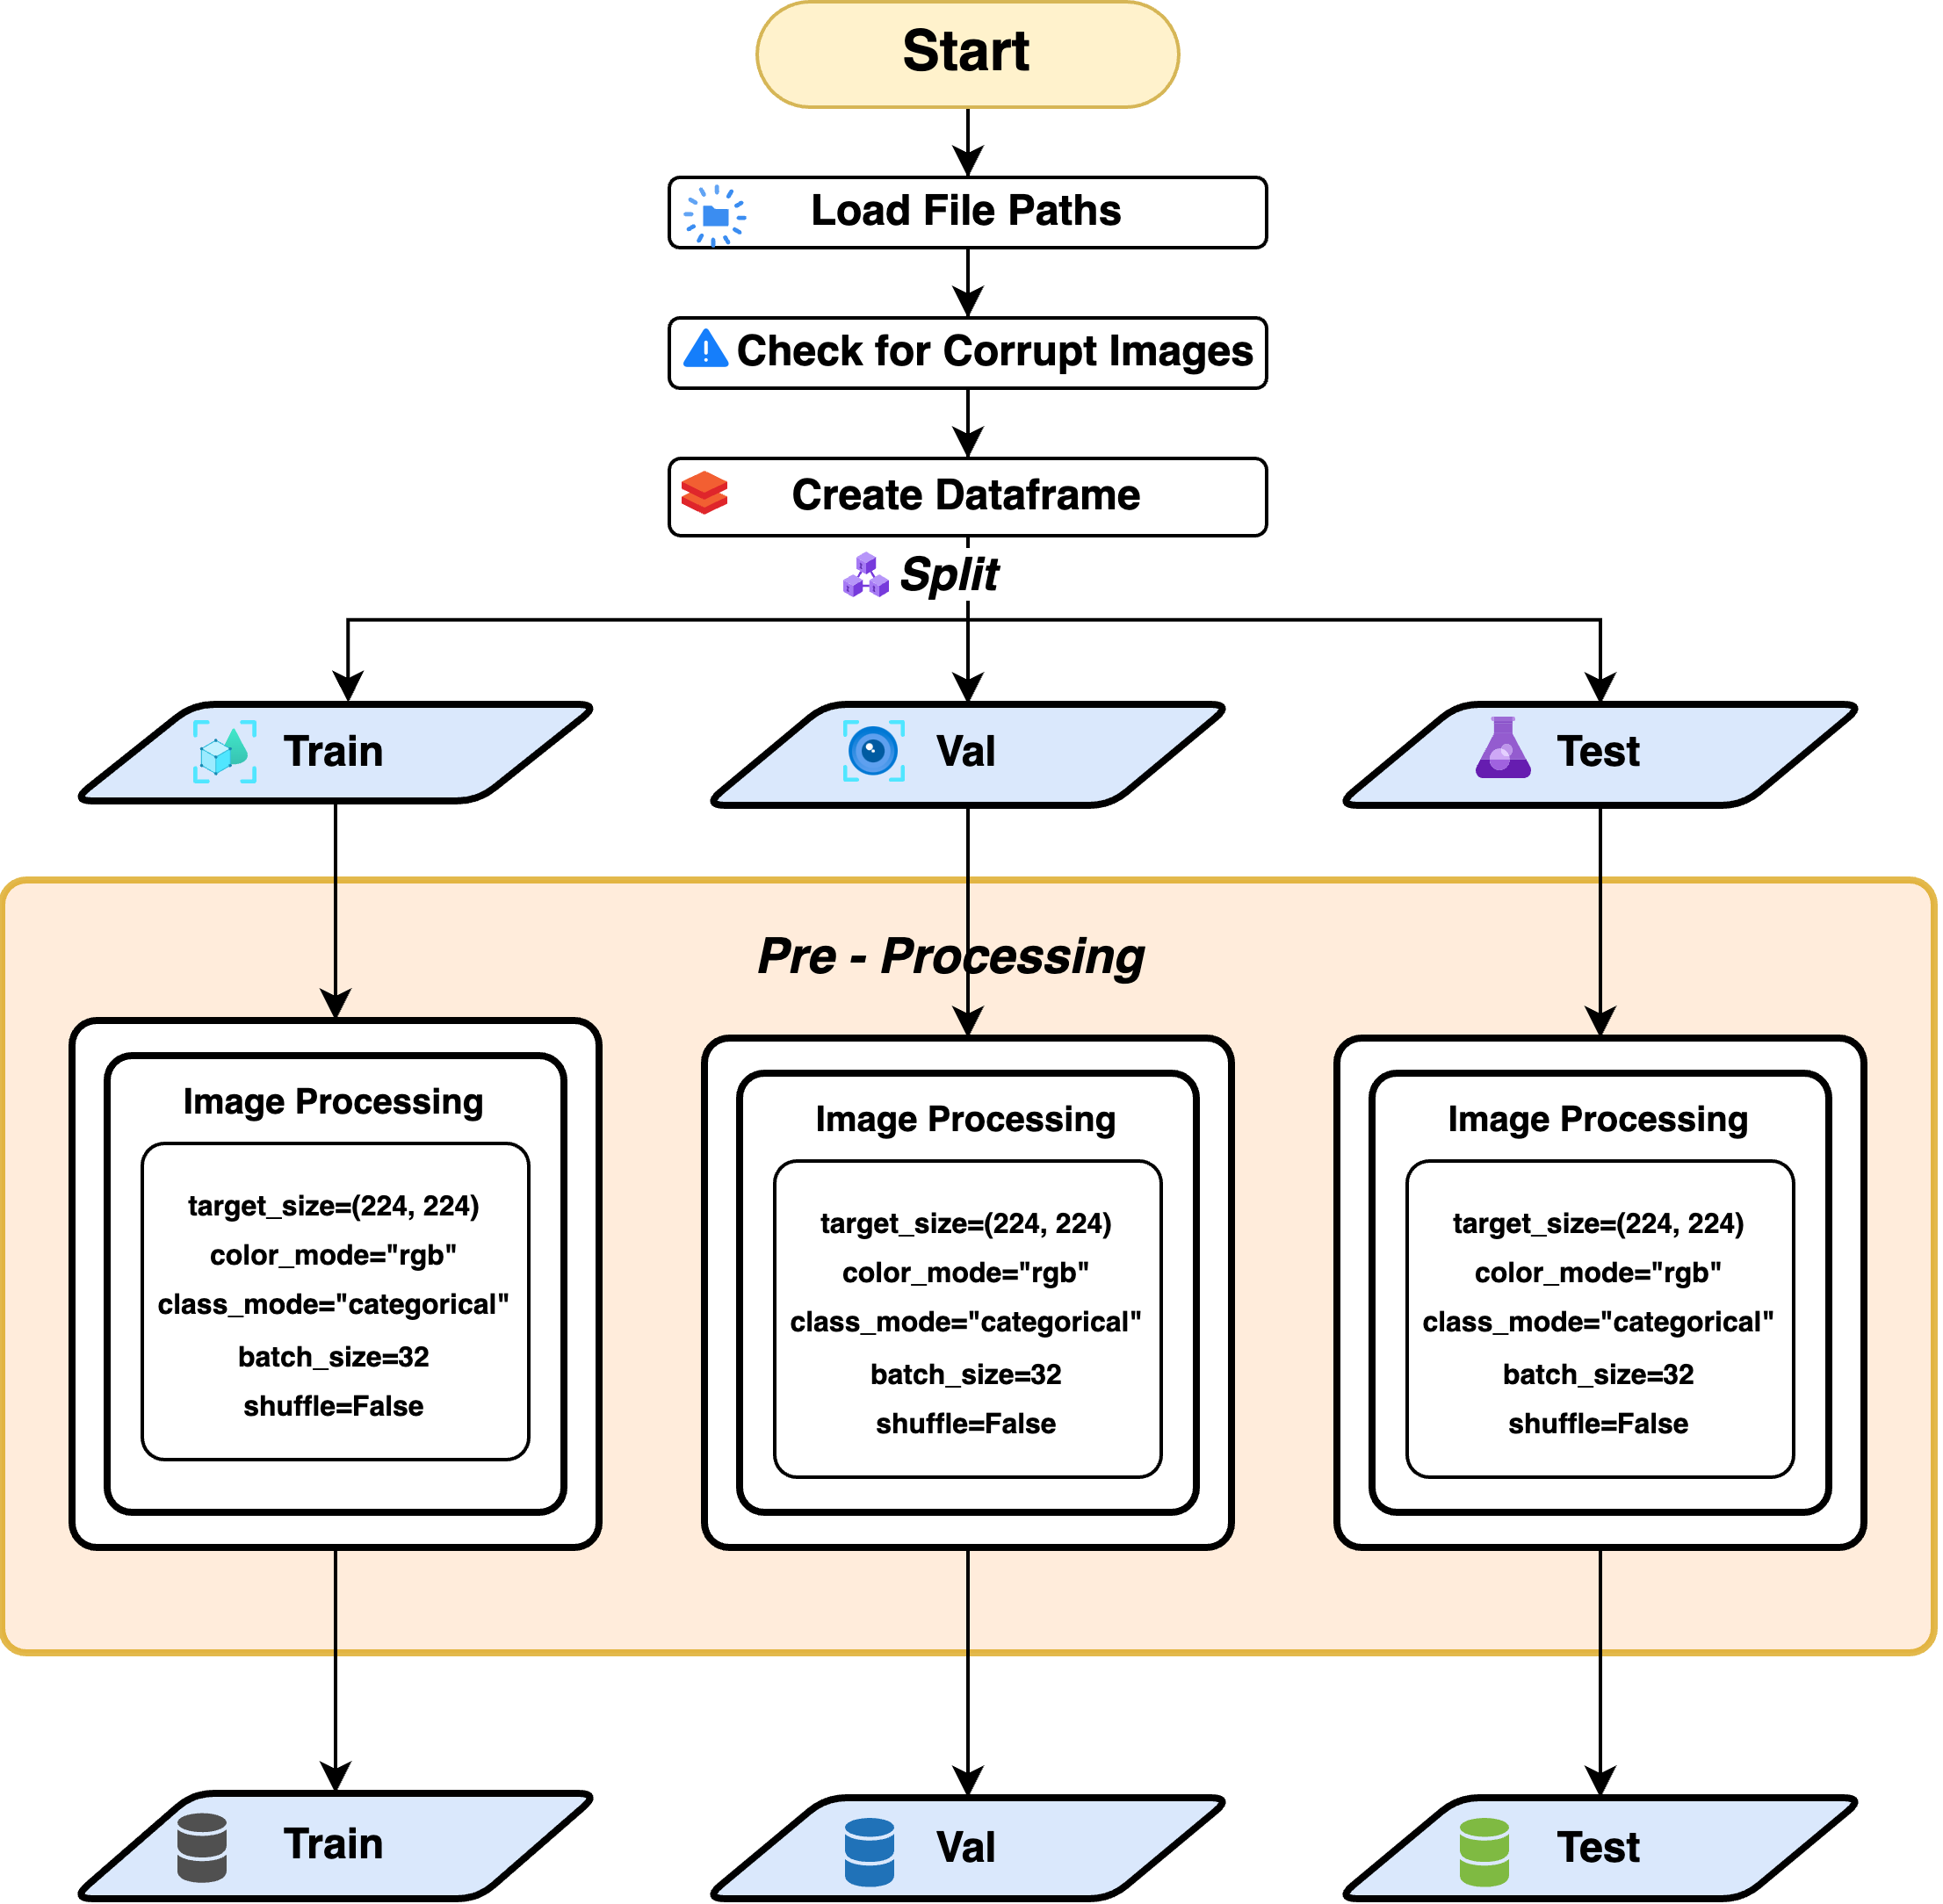
\includegraphics[width=0.8\columnwidth]{figures/image_preprocessing_full.png}  % Adjust the width to your liking
    \caption{pre-processing flow} % Caption for the image
    \label{fig:image_preprocessing_full} % Label to reference the image later in the document
\end{figure}

In order for the model to learn from the patterns in the images it is very import that the images are being processed properly. Data is processed so that the model can learn from it in a efficient and effective way. Figure \ref{fig:image_preprocessing} shows the steps applied on the images so that it can compatible with the model, and read as much details as possible but at the same time be efficient in learning from it.

\subsection{Data Cleaning}
\begin{figure}[h!]
    \centering
    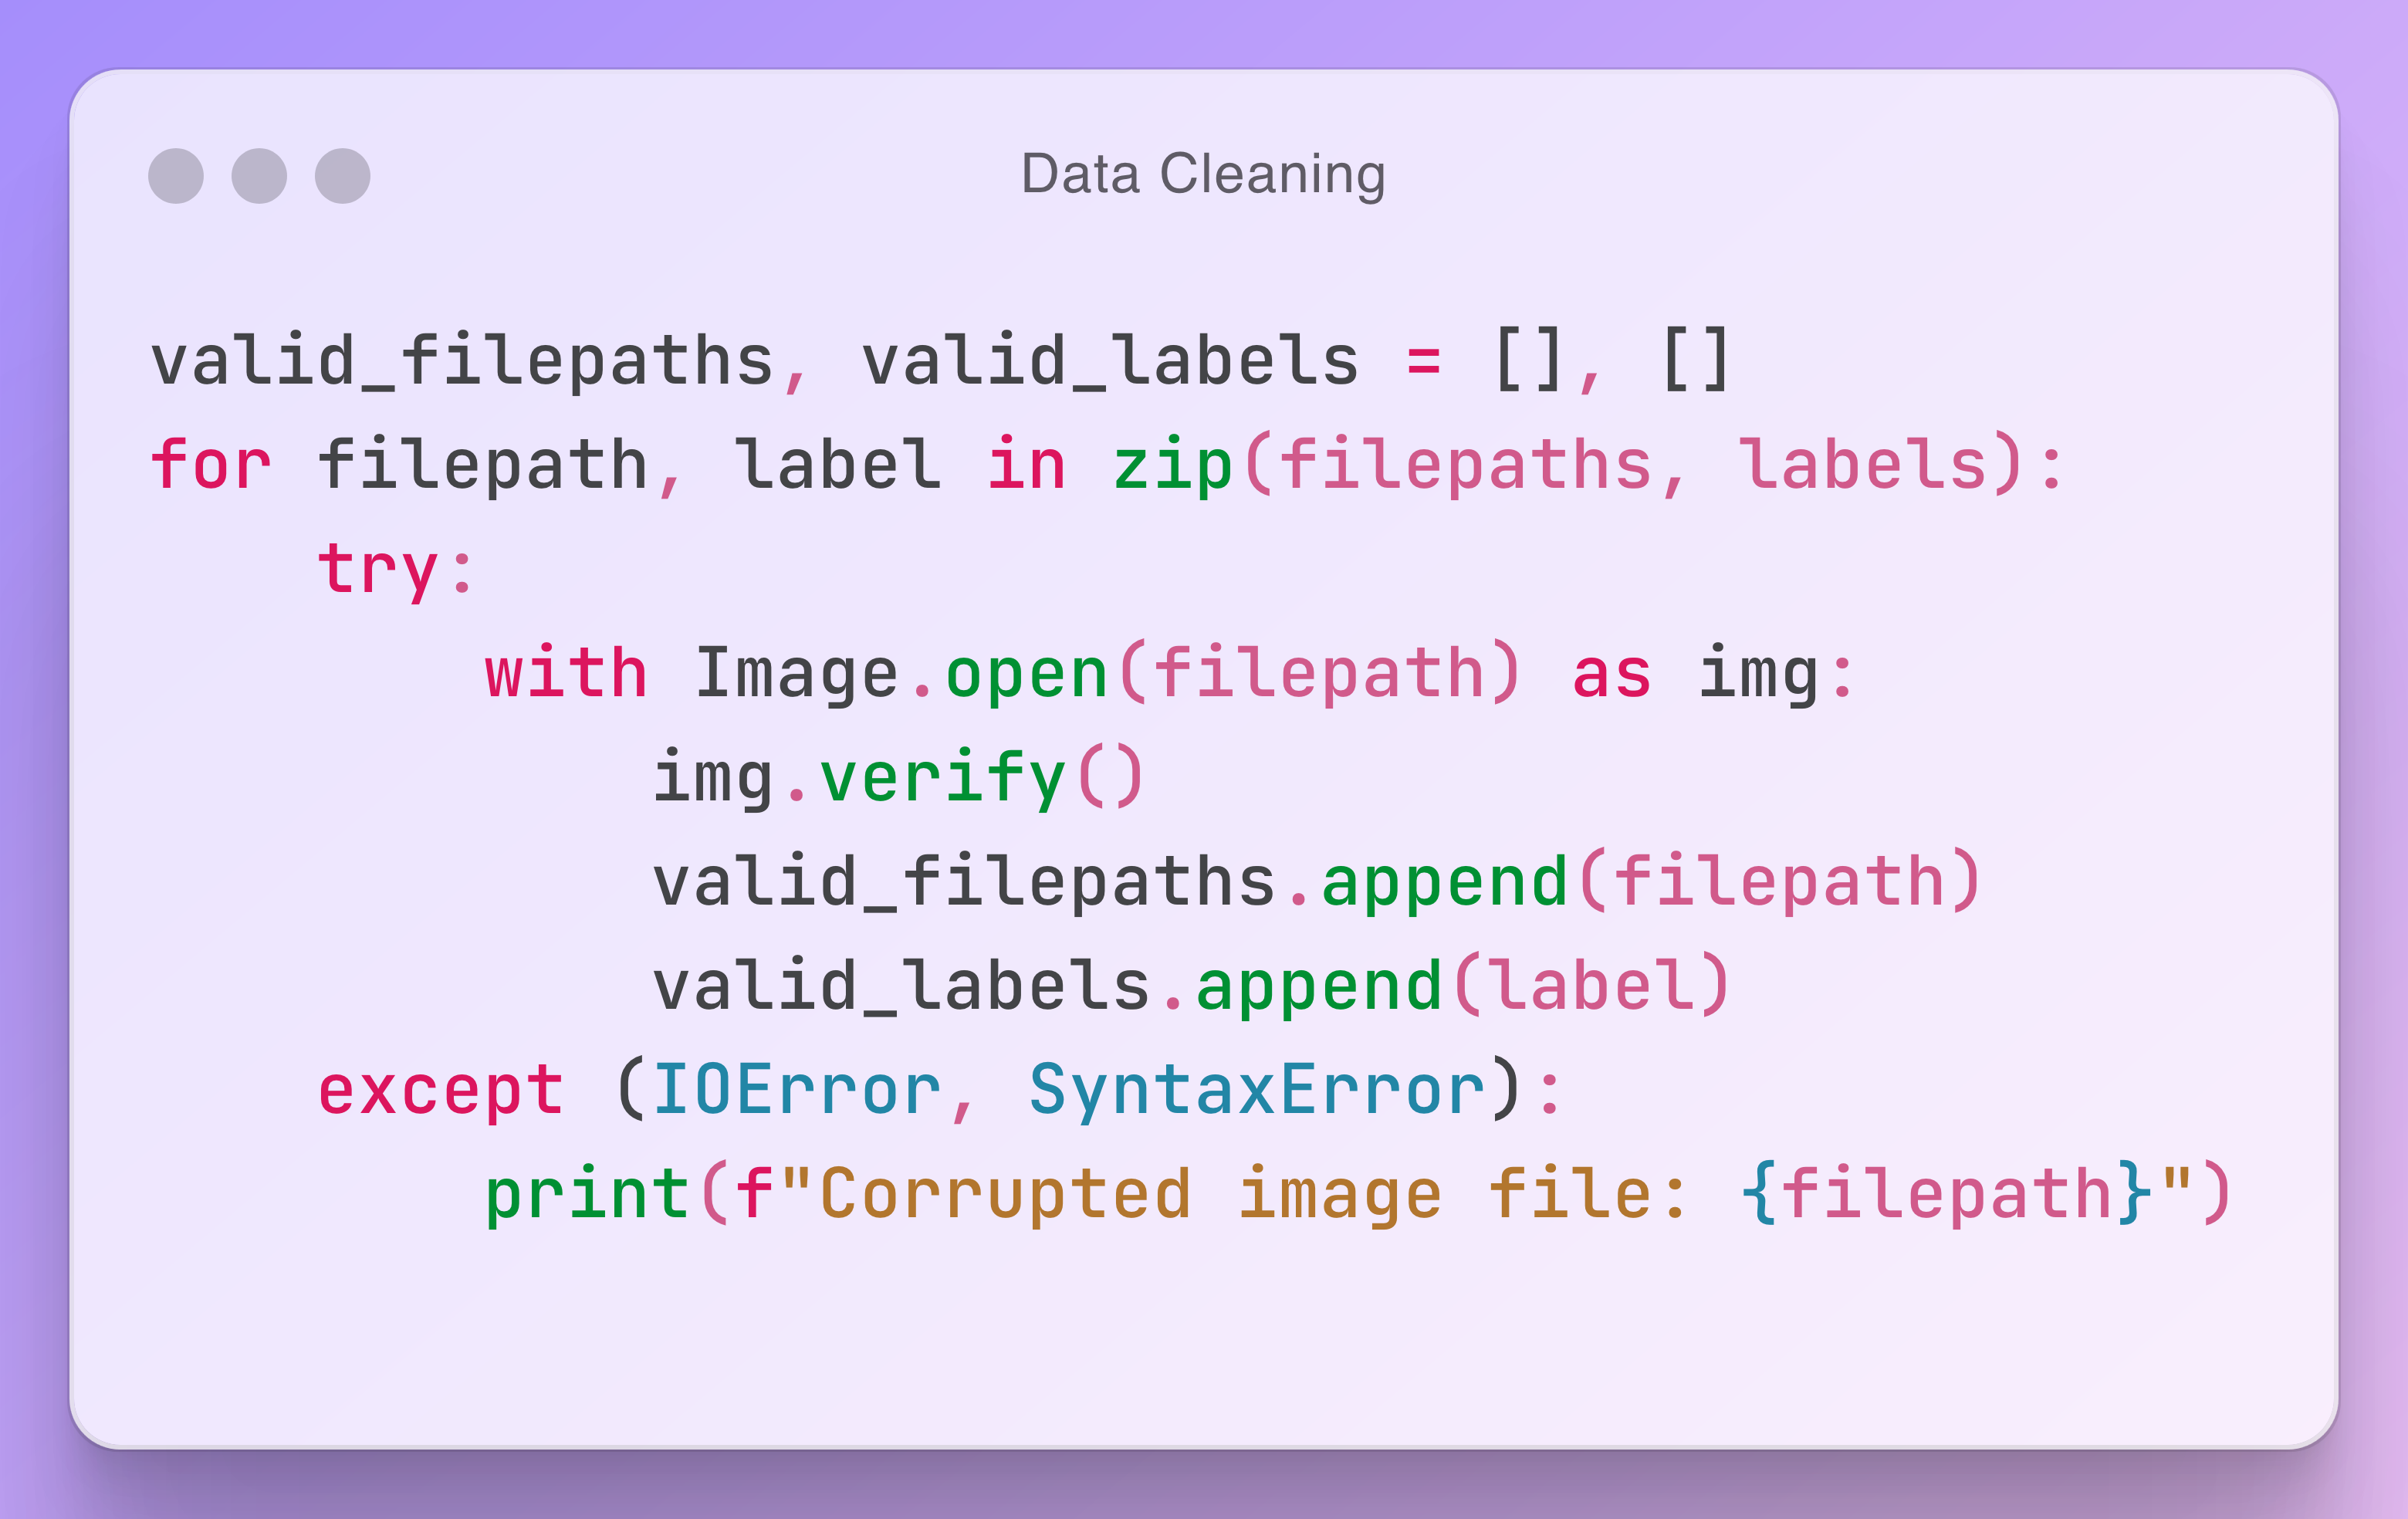
\includegraphics[width=0.8\columnwidth]{figures/data_cleaning.png}  % Adjust the width to your liking
    \caption{Dataset cleaning} % Caption for the image
    \label{fig:dataset_Cleaning} % Label to reference the image later in the document
\end{figure}
In this step the corrupt image will be removed if incase any are found. But in this particular dataset we were not getting error. Hence none of the image were deleted from the dataframe.

\subsection{Data Resizing}
The images are resized into the size of to $224 \times 224$ pixels. This is because the model that we are using i.e. EfficientNet-B0 are designed for a specific image size that is $224 \times 224$ pixels. That is because EfficientNet-B0 uses compound scaling method where the width of the network, depth and the resolution are uniformly scaled. If the input sizes are changed the performance and the efficiency of model will be hampered. And accuracy of the model will be lowered. And if higher pixels are used then there will not be any performance gains but just extra effort while training the data . Hence we have to scale it down to that size \cite{tan2019efficientnet} \cite{efficientnet_medium} \cite{keras_efficientnet}. While it is possible to input the sizes like  $244 \times 244$ the performance of the model will be degrading hence it is better to get the input size as the one that is well optimized for for the best results. 

\subsection{Color Mode}
The image color is chosen to be in RGB more. Generally, the color in all the digital images and displays is usually RGB (Red, Green, Blue). By using these three primary colors in different intensities, the model will be able to find patterns in a wider range of hues \cite{epackprinting_rgb}. RGB is considered to be a standard right now as input for many trained convolution neural networks (CNNs) \cite{dsp_rgb_hsv}. Using RGB images guarantees compatibility with these models, allowing for transfer learning and the utilization of pre-existing architectures. In many image identification tasks, color is an essential element. Because RGB photos preserve all the color information, models may recognize and learn complex patterns from color fluctuations much better than using the black-and-white color modes. This is especially beneficial for image classification tasks.

\subsection{Class Mode}
So the generator is told to give one-hot encoded labels,' where each label will have its own unique pattern in vector form \cite{loss_functions_image_classification}. Only one indices in the vector will have value other indices will be zero. That way the model will be able to understand which image is of which class. Training models with categorical is a common loss function in the case of multi-class classification.\cite{generalization_cross_entropy} The categorical cross-entropy loss function, commonly used in multi-class classification, goes well with one-hot encoded labels. This loss function efficiently calculates the difference between the actual distribution and the predicted probability distribution. Hence, by utilizing category labels, the model can generate a probability distribution for all categories \cite{robust_multiclass_classification}.

\subsection{Batch size}
In the preprocessing step a batch size of 32 is chosen for training. This will ensure that there is a balance between computational efficiency and model performance. Smaller batch sizes like 32 offer a trade-off between efficiency and gradient stability, potentially helping escape local minima and generalize better. They fit within modern GPUs’ memory constraints while maintaining stability \cite{keskar2017largebatchtrainingdeeplearning}. Larger batch sizes will be even though smoother it will require require alot more more memory and there is a high risk of overfitting.Additionally, batch size affects convergence speed, allowing sufficient weight updates without excessive overhead, balancing training speed and learned representation quality \cite{masters2018revisitingsmallbatchtraining}.

\subsection{Normalization}
The images are preprocessed using\texttt{preprocess\_input} normalization for the model, this is by using the  function from the EfficientNet library itself. This was used so that input images are properly scaled as required by the model itself. This ensures that the images are standardized by transforming pixel values into a range that aligns with the data the model was trained on. This kind of normalization becomes very much important in deep learning models to that it can improve the performance and efficiency of the models\cite{tan2019efficientnet}.

The approach used in EfficientNet's \texttt{preprocess\_input} function will rescale values of the pixelfrom their original range of $[0, 255]$ to $[-1, 1]$. In this process it subtracts the mean and divided it by the standard deviation of pixel values.The formula for normalization is:

\[
\text{Normalized Pixel Value} = \frac{\text{Pixel Value} - \mu}{\sigma}
\]

where:
\begin{itemize}
    \item $\mu$ represents the mean of the pixel values across the dataset.
    \item $\sigma$ stands for the standard deviation of the values of the pixel values across the dataset.
\end{itemize}

Normalizing the image will ensures that all input data will lie withing a similar scale this will prevent the issues issues like convergence caused due to having large variations in input magnitudes \cite{he2015delving}.

\section{Proposed Model Architecture}
This section outlines the about the model architecture that is used for this research. The model of choice for this task is EfficientNetB0, because it is a very powerful and efficient pertained model which as it's names suggest's is very efficient and requires less computing power without compromising the final results. It will extract that features and then can be used to include uncertainty estimation into the pipeline.  This will help in improving the reliability in these models for the clinical environment.

\subsection{Base Model Architecture}
\begin{figure}[h!]
    \centering
    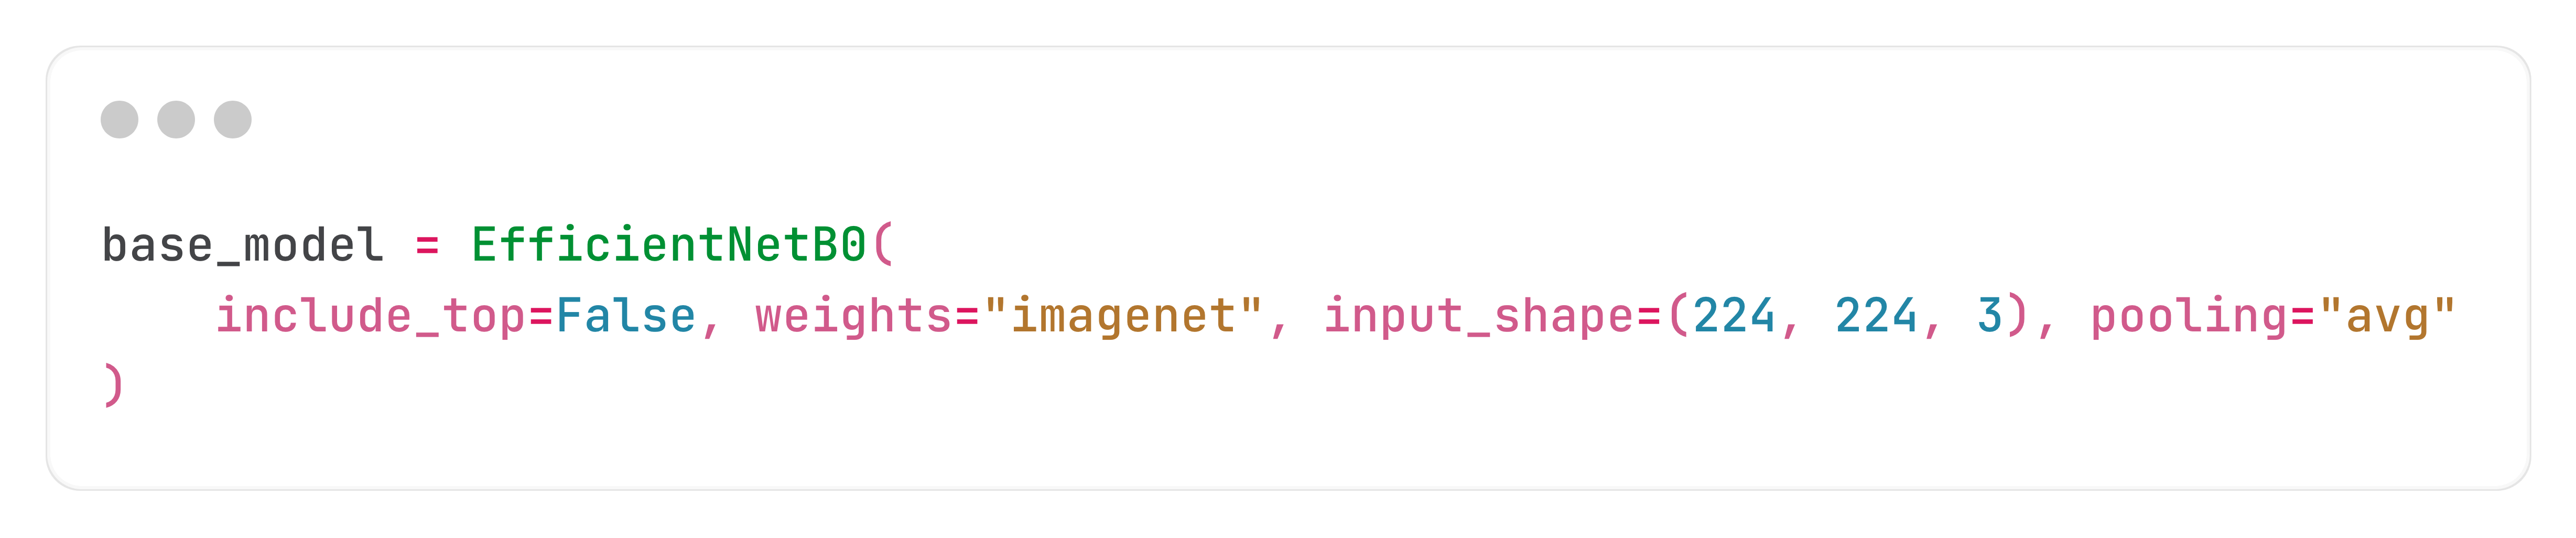
\includegraphics[width=0.8\columnwidth]{figures/res_model_base.png}  % Adjust the width to your liking
    \caption{Model Base} % Caption for the image
    \label{fig:base model} % Label to reference the image later in the document
\end{figure}
EfficientNet is considered to be one among the best models in the world on Convolution Neural Network. It is known to be one of the best models made for these sort of tasks which is able to do it much more efficiently but not compromising the performance. EfficientNetB0 known for its efficient scaling of depth, width, and resolution and it is used as backbone of the proposed model \cite{2021Hoang}. The network will be initialized with pre-trained ImageNet weights so as to make use of the transfer learning. The architecture includes global average pooling at the output of the backbone, followed by a fully connected layer with 128 neurons and a ReLU activation function. A Dropout layer with a rate of 0.3 is introduced to prevent overfitting. And the input shape of the images will be set to $224 \times 224$ pixels as expected by the EfficientNetB0 model for best performance.

\subsection{Adding Uncertainty Estimation}
As seen in the paper that have been working on Alzheimer’s detection problem, inclusion of uncertainty/confidence parameters for the output to show the confidence of the models is something that is used little to none. Inclusion of this parameter will give the clinicians an idea of how confidently the model is been able to classify the image into that class. In this study to quantify uncertainty, Monte Carlo (MC) Dropout is been used during inference step. Monete Carlo is choosen as the method to calculate uncertainity because this model does not require additional model training. This means a dropout layer will be included while conducting the prediction to perform multiple stochastic forward passes. To calculate the uncertainty, we use the standard deviation of the predictions across all these passes. Let’s break down the formal definition of uncertainty for a set of $n$ forward passes:

\begin{equation}
\sigma = \sqrt{\frac{1}{n} \sum_{i=1}^{n} (p_i - \bar{p})^2},
\end{equation}
here $p_i$ stands for the prediction for the $i$-th forward pass, and $\bar{p}$ is the mean prediction.

The uncertainty value is then converted to a confidence score deducting the uncertainty score by 1. This is because the uncertainty and confidence are inversely promotional. Hence by deducting the value we get a  confidence score of the model. Confidence score is calculated using the below formula:

\begin{equation}
    C = 1 - \sigma,
\end{equation}
where $C$ represents the confidence score and $\sigma$ is the uncertainty score that is calculated using the previous formula. 
To determine whether a prediction is reliable or not, a confidence score threshold of 0.2 is selected. The model's prediction is considered as confident if the score is greater than 0.8 and anything below will be considered.



\subsection{Output Layer}
\begin{figure}[h!]
    \centering
    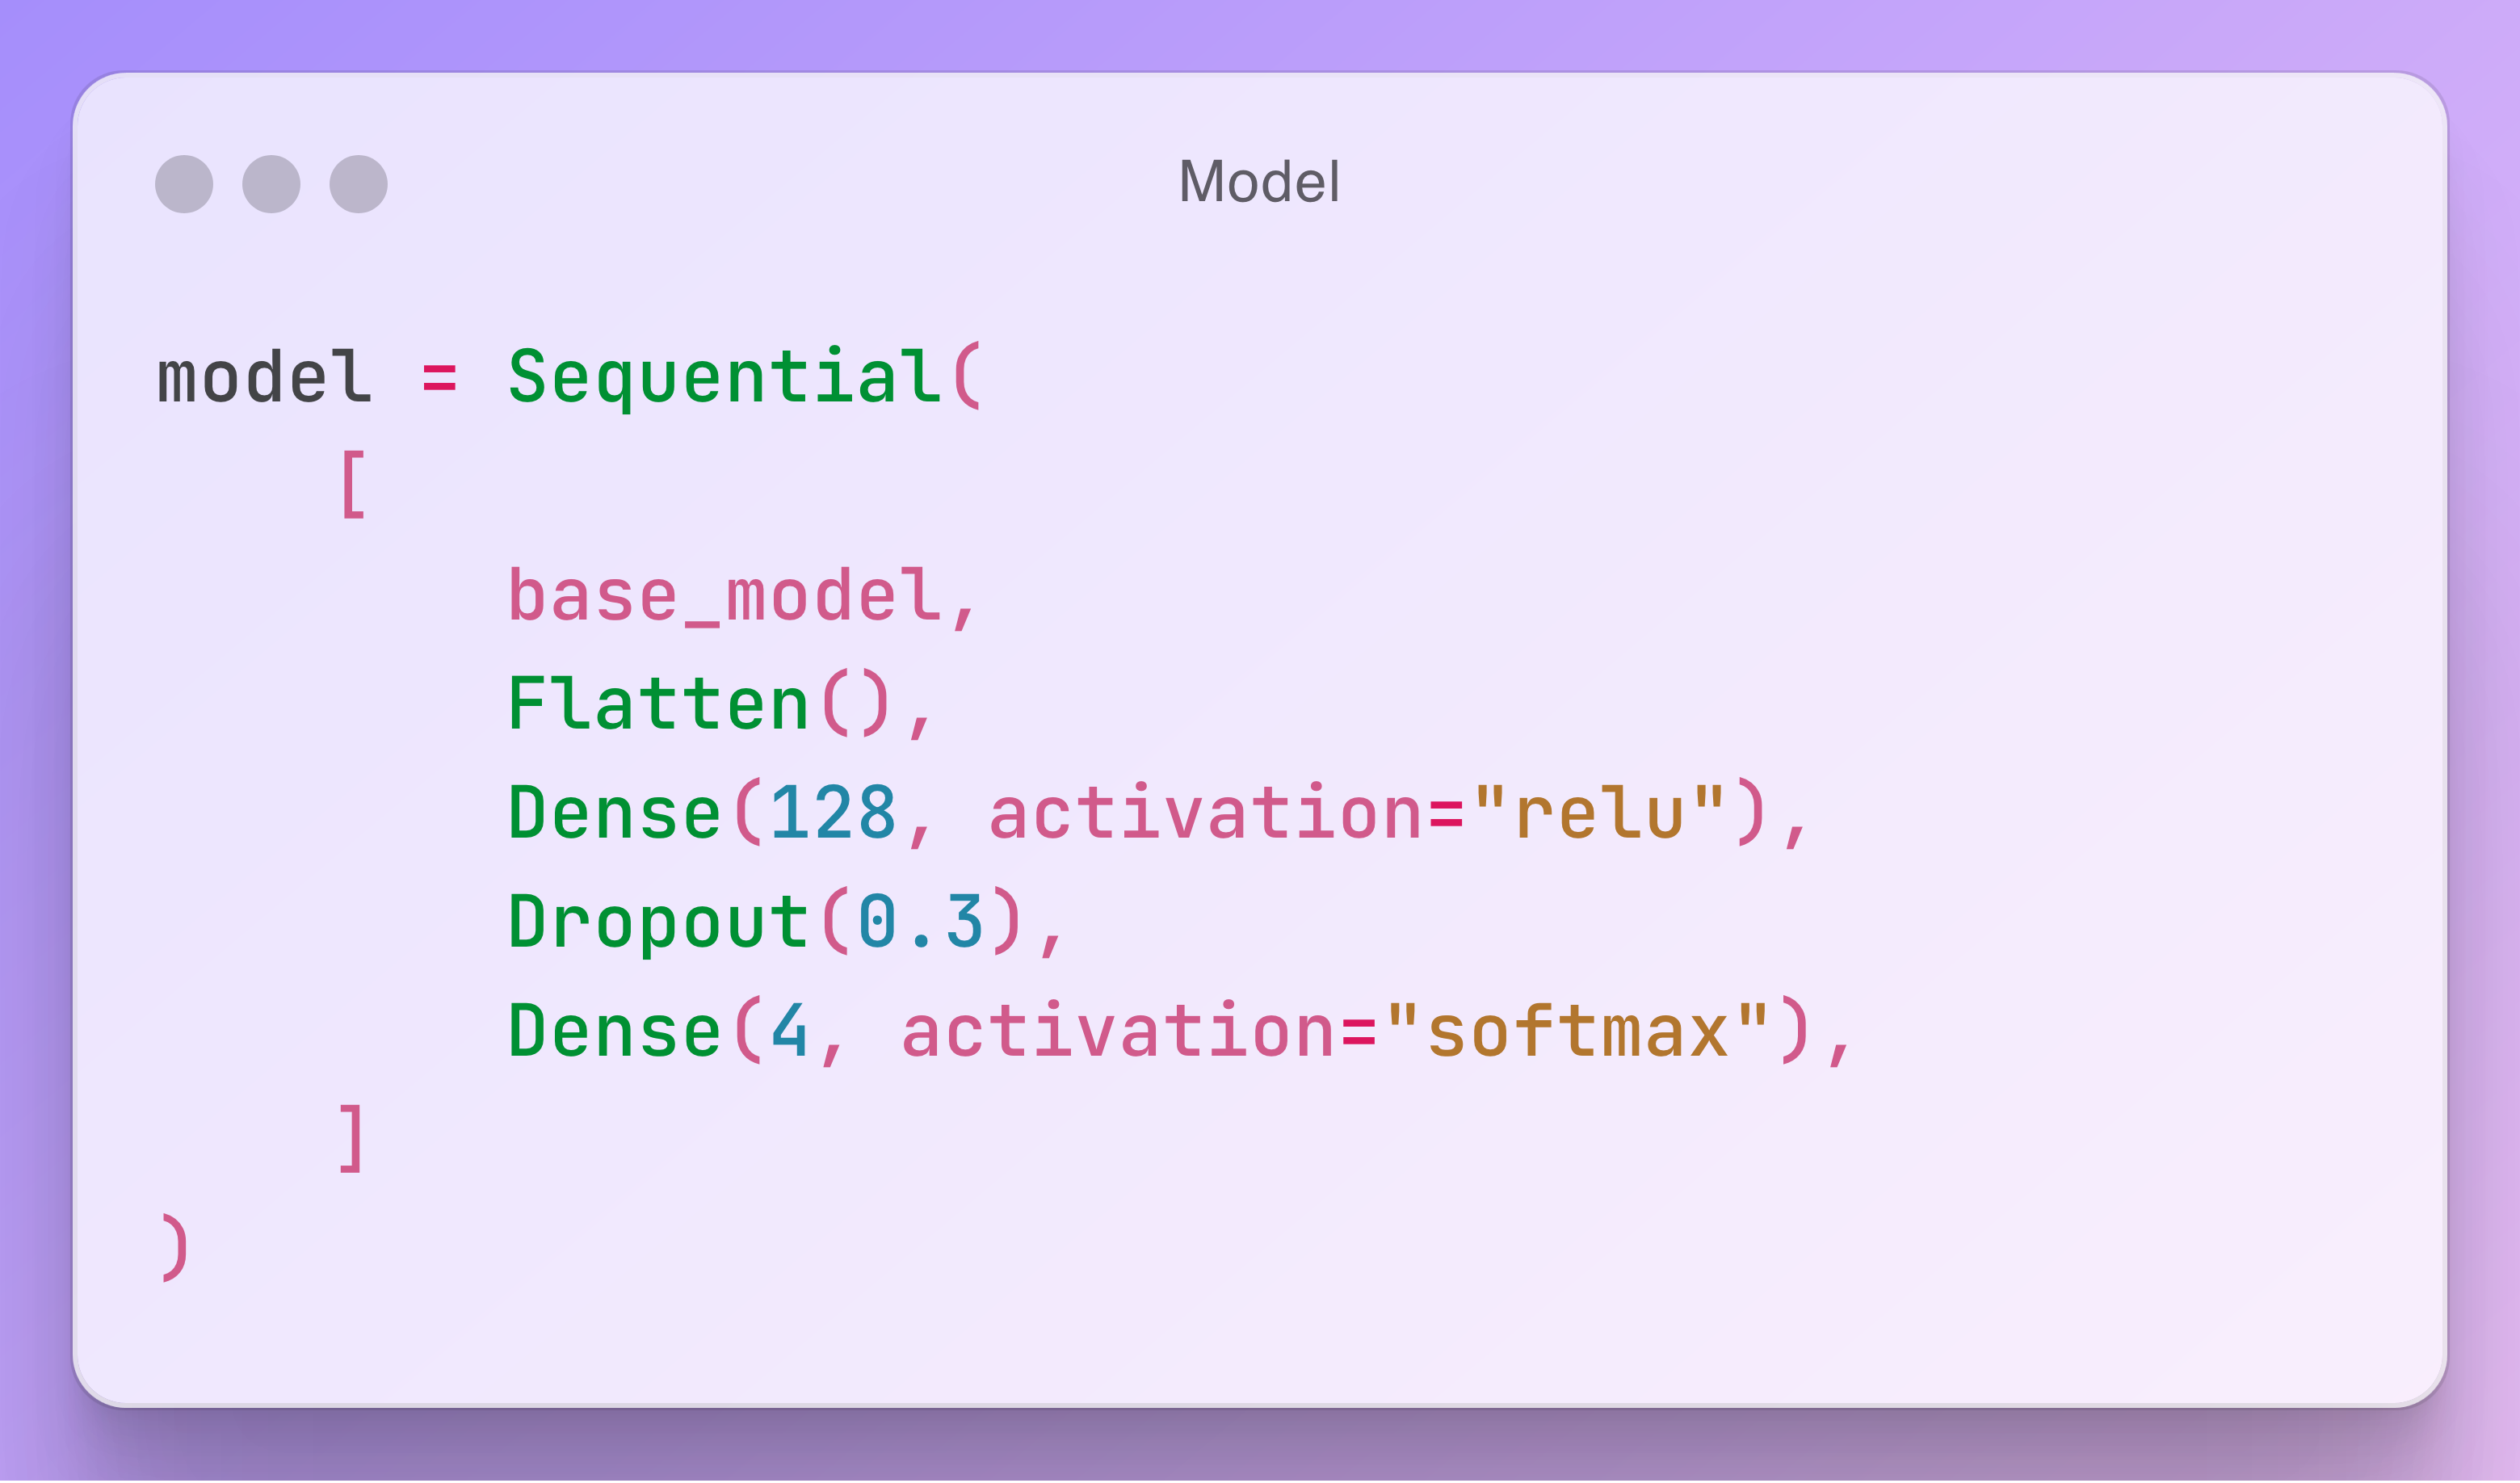
\includegraphics[width=0.8\columnwidth]{figures/model_sequential.png}  % Adjust the width to your liking
    \caption{Model sequential} % Caption for the image
    \label{fig:sequential model} % Label to reference the image later in the document
\end{figure}
The output layer has 4 neurons. This is because there are four different classes that the model will be predicting. Hence there are four neurons. The activation layer user for the final output layer is 'softmax'. The output layer will be creating probability scores for each class: NonDemented, MildDemented, VeryMildDemented and ModerateDemented. 

\subsection{Training and Evaluation}
The model is compiled using the Adamax optimizer with a learning rate of 0.001. The categorical crossentropy loss function is employed to optimize multi-class classification performance. Early stopping and learning rate reduction strategies are implemented to ensure robust convergence.

The model is trained on the training dataset for $N$ epochs with validation monitoring. Performance metrics, including accuracy, precision, recall, and F1 score, are computed on the test dataset. Monte Carlo predictions are utilized during evaluation to derive the mean prediction and uncertainty values.


\section{Model Training and Optimization}
\begin{figure}[h!]
    \centering
    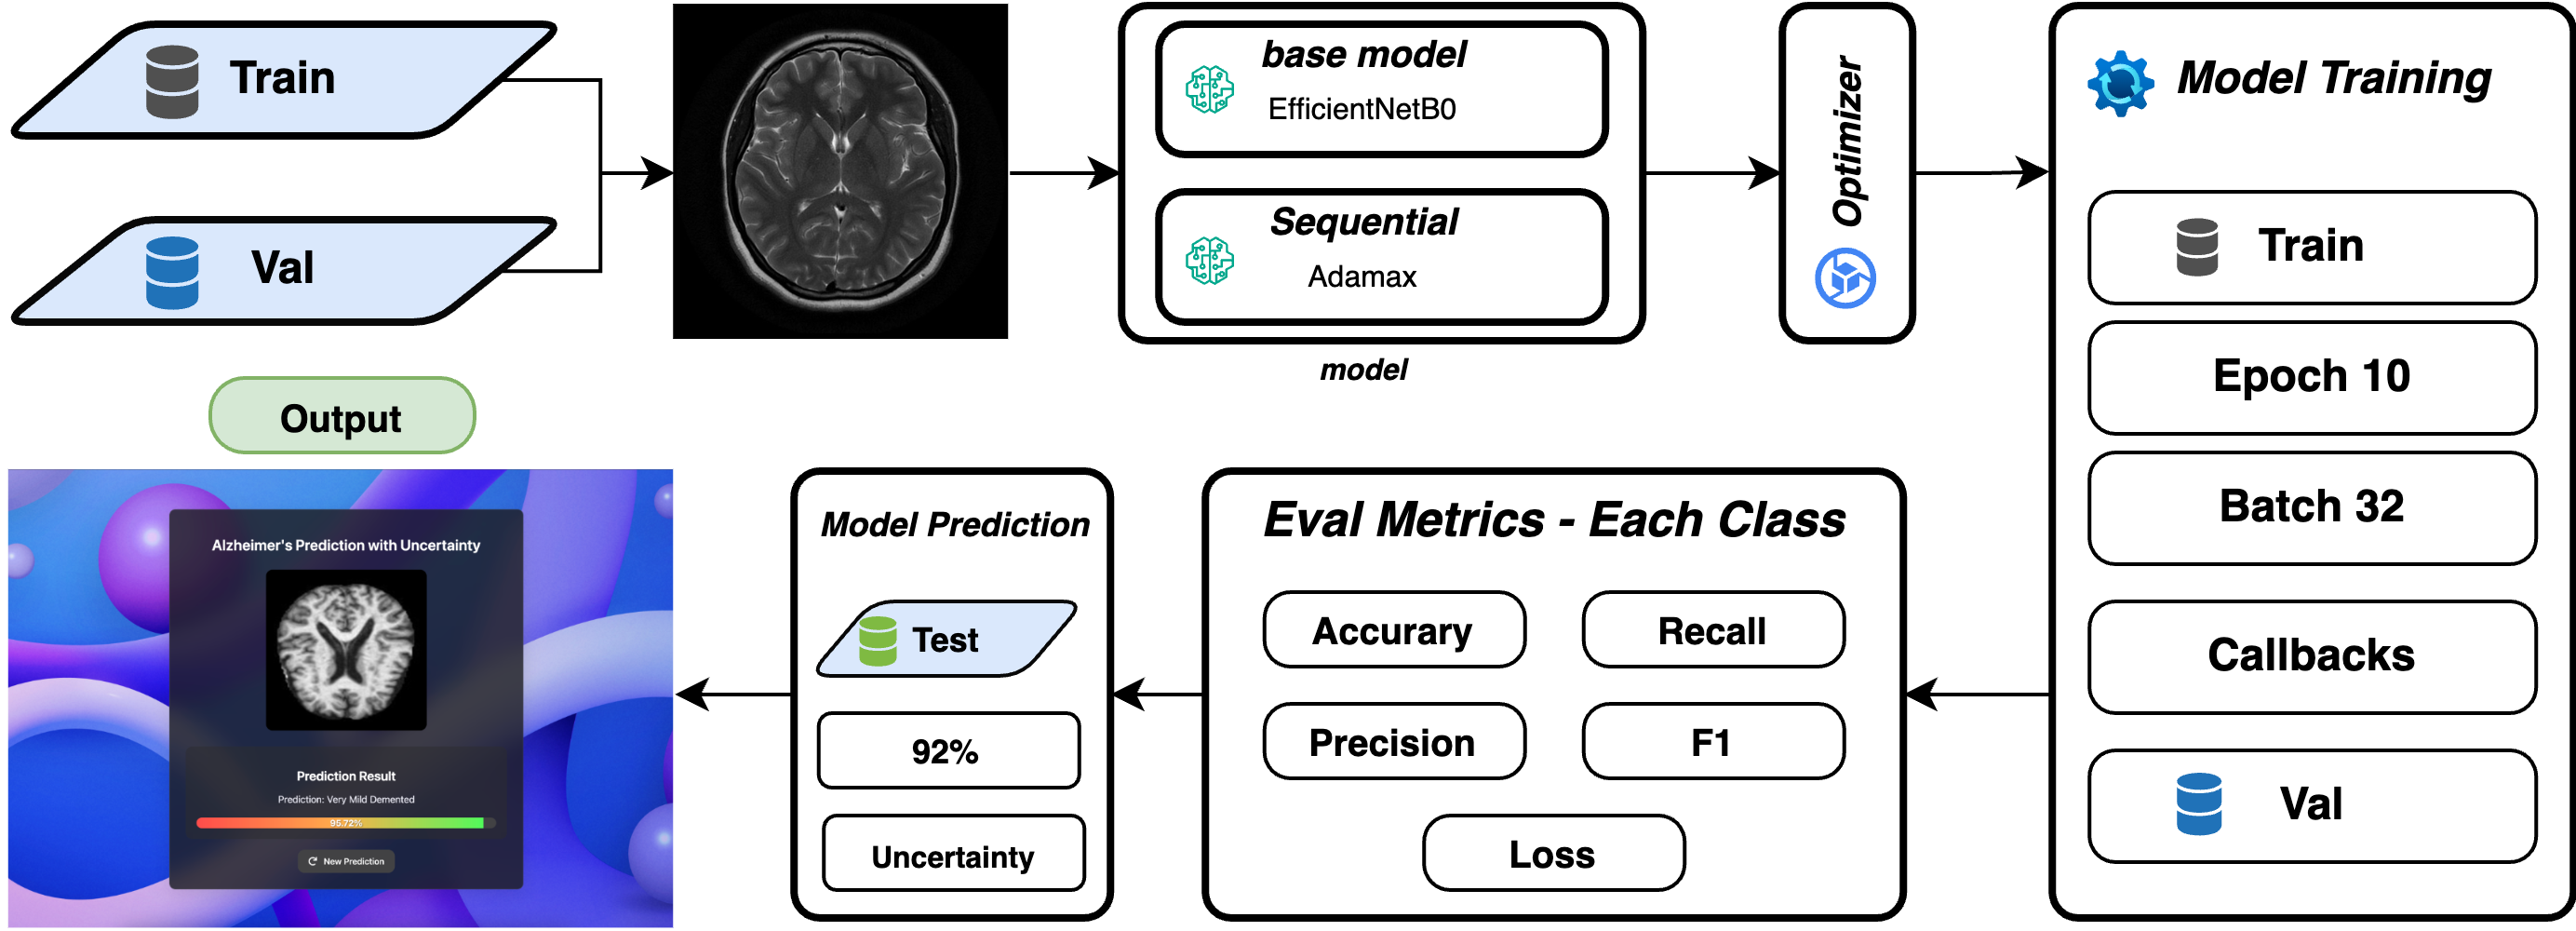
\includegraphics[width=1.0\columnwidth]{figures/model_training_optimization.png}  % Adjust the width to your liking
    \caption{Flow of model training and output} % Caption for the image
    \label{fig:model training} % Label to reference the image later in the document
\end{figure}



\subsection{Training Configuration}
This step is consider to be the most critical steps in the machine learning process. How model is configured has a huge impact on the models perfomance on the final task as well as the efficiency of the model while training as well while predicting the results. The model used here make use of the Adamax optimizer. It is a variant of the Adam optimizer. But we make use of Adamax optimizer particularly because Adamax is suits extremely well for the sparse gradients and high dimensional data.So it fit's well for the image dataset that we are using. The learning rate is set to \(0.001\). In several studies it has been showed that learning rate of \(0.001\) balances convergence speed and model stability as it has been demonstrated in prior studies to balance convergence speed and model stability \cite{2017Kingma}. The categorical crossentropy loss function is utilized as this is a multi class classification. It has proved to be very effective for the multi-class classification.The Formula for categorical crossentropy is as follows \ref{eq:categorical_crossentropy}:

\begin{equation}
    L = -\sum_{i=1}^{N} y_i \log(\hat{y}_i),
    \label{eq:categorical_crossentropy}
\end{equation}
here \(y_i\) stands for the true label, and \(\hat{y}_i\) stands for the predicted probability for the \(i\)-th class.

\subsection{Optimization Strategies}
To improve the model's generalization, the proposed model introduces two optimization strategies: Early Stopping and Learning Rate reduction

\subsubsection{Early Stopping}
Introduction of the Early stopping while training model will make sure the the validation loss in always monitored. And when performance of the validation set does not improve it will stop the training, once the patience period is reached. This will ensure that the model is not overfitted for the test model. This is improve the generalizability of the model. And also this will prevent the unnecessary computation power that is required \cite{1996Lutz}. The patience parameter is set to five epochs. The parameter \texttt{restore\_best\_weights} will make sure thaat model always comes back to it's best-performing weights. This is an example algorithm \ref{alg:early_stopping} showing the same.

\begin{algorithm}[h]
\caption{Early Stopping}
\label{alg:early_stopping}
\begin{algorithmic}[1]
\State Set's patience \( p \) to 0
\For{every epoch}
    \If{Validation loss improves}
        \State Saves the model weights
        \State Resets patience \( p \) equals 0
    \Else
        \State Increments patience \( p \) by 1
    \EndIf
    \If{p is >= to patience}
        \State Training will be Stopped
    \EndIf
\EndFor
\end{algorithmic}
\end{algorithm}

\subsubsection{Learning Rate Reduction on Plateau}
If the learning rate doesn’t improve for three epochs in a row, we decrease it by half. This way, the model finds a better local minimum and keeps training stable. \cite{2017Loshchilov} says this method works really well. After the reduction, we calculate the new learning rate \(lr_t\) as follows:

\begin{equation}
    lr_t = \max(f \cdot lr_{t-1}, lr_{\text{min}}),
\end{equation}
where \(f\) is the reduction factor, \(lr_{t-1}\) is the learning rate in the previous epoch, and \(lr_{\text{min}}\) is the minimum allowable learning rate.

\subsection{Training Process}
The model training process was done using 10 epochs, on the training set and then it is validated on the validation set. So that model can be evaluated on each epoch. The history which training will be saved which included parameters such as accuracy, loss information. These evaluation are being saved for both the sets i.e. training set as well as the validation set.Table \ref{tab:training_parameters} give a overall summary.

\begin{table}[h]
    \centering
    \caption{Training Parameters and Configuration}
    \label{tab:training_parameters}
    \begin{tabular}{|l|l|}
        \hline
        \textbf{Parameter} & \textbf{Value} \\
        \hline
        Optimizer          & Adamax \\
        Learning Rate      & 0.001 \\
        Loss Function      & Categorical Crossentropy \\
        Early Stopping Patience & 5 epochs \\
        Learning Rate Reduction Factor & 0.5 \\
        Minimum Learning Rate & \(1 \times 10^{-6}\) \\
        Epochs             & Set to 10 but it is Dynamic (Based on Early Stopping) \\
        \hline
    \end{tabular}
\end{table}

\section{Evaluation Metrics}

To evaluate the performance of the base as well as the proposed model, we will be taking into account several metrics. They are  accuracy, precision, recall, F1-score, macro average and weighted average. This will allows to get a very detailed understand of the models performance. Additionally because this is a multi class classification this thesis put light to the evaluation metrics on each classes to that it records how well it performs for each class. These metrics will provide a detailed view of how well the model is being able to make predictions for each class. Furthermore, uncertainty evaluation is being implemented in this thesis. This is something that was not included in the base model. Tell me give us idea about how confident the model is when it comes to predicting the values.

\subsection{Accuracy}
Accuracy is a very important metric while evaluating classification models, in this case a multi class classification model. Accuracy shows the ratio of correct predictions to the total number of predictions made. The formula used to calculate accuracy is as follows:

\begin{equation}
    \text{Accuracy} = \frac{\text{No. of correct predictions}}{\text{Total no. of predictions}} = \frac{\sum_{i} I(y_{\text{pred},i} = y_{\text{true},i})}{N},
\end{equation}
here \( y_{\text{pred},i} \) stands for the predicted label \( i \), \( y_{\text{true},i} \) stands for the true label, and \( N \) is the total number of samples.

\subsection{Precision}
Precision metrics will find a proportion of positive predictions that are that are actually positive. It is important for this thesis because the cost of false positive can be very risky. When it comes to medical diagnosis a false positive prediction can lead to unnecessary medications and treatments. And since the dataset is moderately imbalanced this evaluation metrics becomes very important. The formula for calculating Precision is as follows:
\begin{equation}
    \text{Precision} = \frac{TP}{TP + FP},
\end{equation}
where \( TP \) represents true positives and \( FP \) represents false positives.
In our case of Alzheimer’s diagnose it becomes important because minimizing false positive is very important to avoid over diagnosis.

\subsection{Recall}
Recall is also called sensitivity or true positive rate. Recall will be measuring the proportion of actual positive class that are correctly identified by the model. In the context of Alzheimer's disease detection, recall indicates the model’s ability to classify all potential Alzheimer’s patients. High recall ensures that fewer true positives are missed, which is crucial for early diagnosis. The formula to calculate Recall is:
\begin{equation}
    \text{Recall} = \frac{TP}{TP + FN},
\end{equation}
where \( TP \) represents true positives and \( FN \) represents false negatives.

In our case of Alzheimer’s classification it becomes where important to check if the model is failing to detect positive case of Alzheimer’s or in other words false positives. Because if the model is failing to tell the class which the patient is in then the disease might go unnoticed and it might worsen at the later stages of his/her life.

\subsection{F1-Score}
F1-score is calculated using all of the above scores. It is a 2 times the multiplication of Precision and Recall and devided by addition of Precision and Recall as shown in the equation. The Formula for F1 score is as follow: 
The F1-score is the harmonic mean of precision and recall, providing a balanced measure of the model's performance. It is particularly useful when dealing with class imbalance, as it considers both false positives and false negatives. The F1-score is defined as:

\begin{equation}
    \text{F1-score} = 2 \cdot \frac{\text{Precision} \cdot \text{Recall}}{\text{Precision} + \text{Recall}},
\end{equation}


\subsection{Confusion Matrix}
By using the confusion matrix we are able to visualize the performance of the model. Confusion matrix visualizes the number of correctly predicted items and incorrectly predicted items across all classes. This will enable to calculate the evaluation metrics like accuracy, recall, precision and F1-score for each class as shown the table \ref{tab:confusion_matrix}.

\begin{table}[h!]
\centering
\begin{tabular}{|c|c|c|c|c|}
\hline
\rowcolor[HTML]{EFEFEF} 
& \multicolumn{4}{c|}{\textbf{Predicted}} \\ \hline
\textbf{True} & \textbf{NonDemented} & \textbf{VeryMildDemented} & \textbf{MildDemented} & \textbf{ModerateDemented} \\ \hline
\textbf{NonDemented} & \cellcolor[HTML]{DFF0D8} TP1 & FN1 & FN2 & FN3 \\ \hline
\textbf{VeryMildDemented} & FP1 & \cellcolor[HTML]{DFF0D8} TP2 & FN3 & FN4 \\ \hline
\textbf{MildDemented} & FP2 & FP3 & \cellcolor[HTML]{DFF0D8} TP3 & FN5 \\ \hline
\textbf{ModerateDemented} & FP4 & FP5 & FP6 & \cellcolor[HTML]{DFF0D8} TP4 \\ \hline
\end{tabular}
\caption{Confusion Matrix for Model Evaluation}
\label{tab:confusion_matrix}
\end{table}

\subsection{Uncertainty Estimation}
Along with all the standard classification metrics that are used in previous researches, in this research models uncertainty while predicting the class in being calculated. For this task the chosen method is Monte Carlo Sampling. For each prediction the model will evaluate multiple times, and the variance which predicting among all samples is used to calculate uncertainty. The predicted mean and the uncertainty is calculated using the below formula:

\begin{equation}
    \text{mean predictions} = \frac{1}{N_{\text{samples}}} \sum_{i=1}^{N_{\text{samples}}} \hat{y}_i,
\end{equation}
\begin{equation}
    \text{uncertainty} = \sqrt{\frac{1}{N_{\text{samples}}} \sum_{i=1}^{N_{\text{samples}}} (\hat{y}_i - \text{mean predictions})^2},
\end{equation}
where \( \hat{y}_i \) represents the \( i \)-th prediction, and \( N_{\text{samples}} \) is the number of Monte Carlo samples \cite{2016Gal}.

In this study, we used 5 samples for each test input, and the predictions with higher uncertainty (above a threshold of 0.2) were identified to assess where the model's confidence is low.

\subsection{Performance Evaluation on Test Set}

The model's performance was evaluated on the test set using the metrics discussed above. The test accuracy was computed and reported, along with the confusion matrix, as shown in Table \ref{tab:confusion_matrix}. Additionally, class-specific metrics such as precision, recall, and F1-score were calculated and displayed in a detailed classification report.

\section{Pipeline Integration}

The final model after all the testing and comparisons in integrated with a Web Application which based on Flask API. This will allow the clinicians to upload the MRI images and get the predictions along with the uncertainty scores. The web application is ready to be deployed and will be accessible through a web browser. You can install the model locally and then move it to a cloud server later. The interface is super easy to use, with a simple way to upload photos and see the predictions. Plus, the uncertainty ratings are shown alongside the predictions, so you can see how reliable the model is. That’s will be a big help for clinicians!

\section{Training environment for Model Comparison}

To make sure that there is farness in comparing the base model and the and the proposed model. Both were run in the Kaggle notebook. Below table shows the system configuration sleeted for training the model. 


\begin{table}[h!]
\centering
\begin{tabular}{|l|l|}
\hline
 & \textbf{Configuration} \\ \hline
\textbf{Platform}   & Kaggle Notebooks       \\ \hline
\textbf{language}   & Python       \\ \hline
\textbf{GPU}        & GPU T4 x2        \\ \hline
\textbf{CPU}        & Intel Xenon  \\ \hline
\textbf{RAM}        & Max 29 GB                  \\ \hline
\end{tabular}
\caption{System configuration}
\end{table}

\section{Implementation}
\label{sec:implementation}
A thesis implementation is what bridges the gap between the theory what is taught about to implement and the practical application of the ideas. It will show how we have turned everything that we have discussed in the Methodology section into code , and it will also explain what steps are taken and the reason behind the choices that are make. It will also include the challenges faced during the implementation phase of the thesis.

Here we will also include the detailed explanation of the environment used for the development, including programming languages, hardware and software specs, and the additional tools used. It explains the steps taken, the choices made, and the reasons behind the approaches chosen. This is to make sure that the others who will be continuing this study can to follow the research and even build on it later on.

Any changes or differences from the original plan will also be covered in the this chapter, along with the reasons for them. So that it gives a realistic view of how practical the suggested solution is by showing how real-world limitations and constraints affect it. This important study shows possible directions for further research and helps us understand the topic better.


\subsection{Data Preparation}
The performance and dependability of machine learning models are greatly impacted by the data preparation stage of implementation. This process includes operations like data cleansing, normalization, transformation, and feature engineering, entails converting raw data into a clear and organized format which is more optimized for the model that chosen. The efficiency of machine learning models is directly impacted by the quality of the input data. Hence it is very important spend enough time and effort on data preparation procedures in order to make sure precise and significant improvement of the models performance. 

To reduce problems like data noise, input size error, data preparation methods are very important. This includes deleting corrupt images, encoding class values using one hot encoding, and normalizing images data according to the requirement of the model.By taking these actions, the model's capacity to efficiently learn from the data is increased, improving its prediction performance. 

In conclusion, careful data preparation is essential to machine learning model deployment success. Practitioners can greatly improve model performance and obtain more precise and useful insights from their studies by guaranteeing data quality and relevance through thorough preprocessing. The data preparation will have these 5 steps:
\begin{itemize}
    \item \textbf{Loading the Images Data}:
    \begin{figure}[h!]
        \centering
        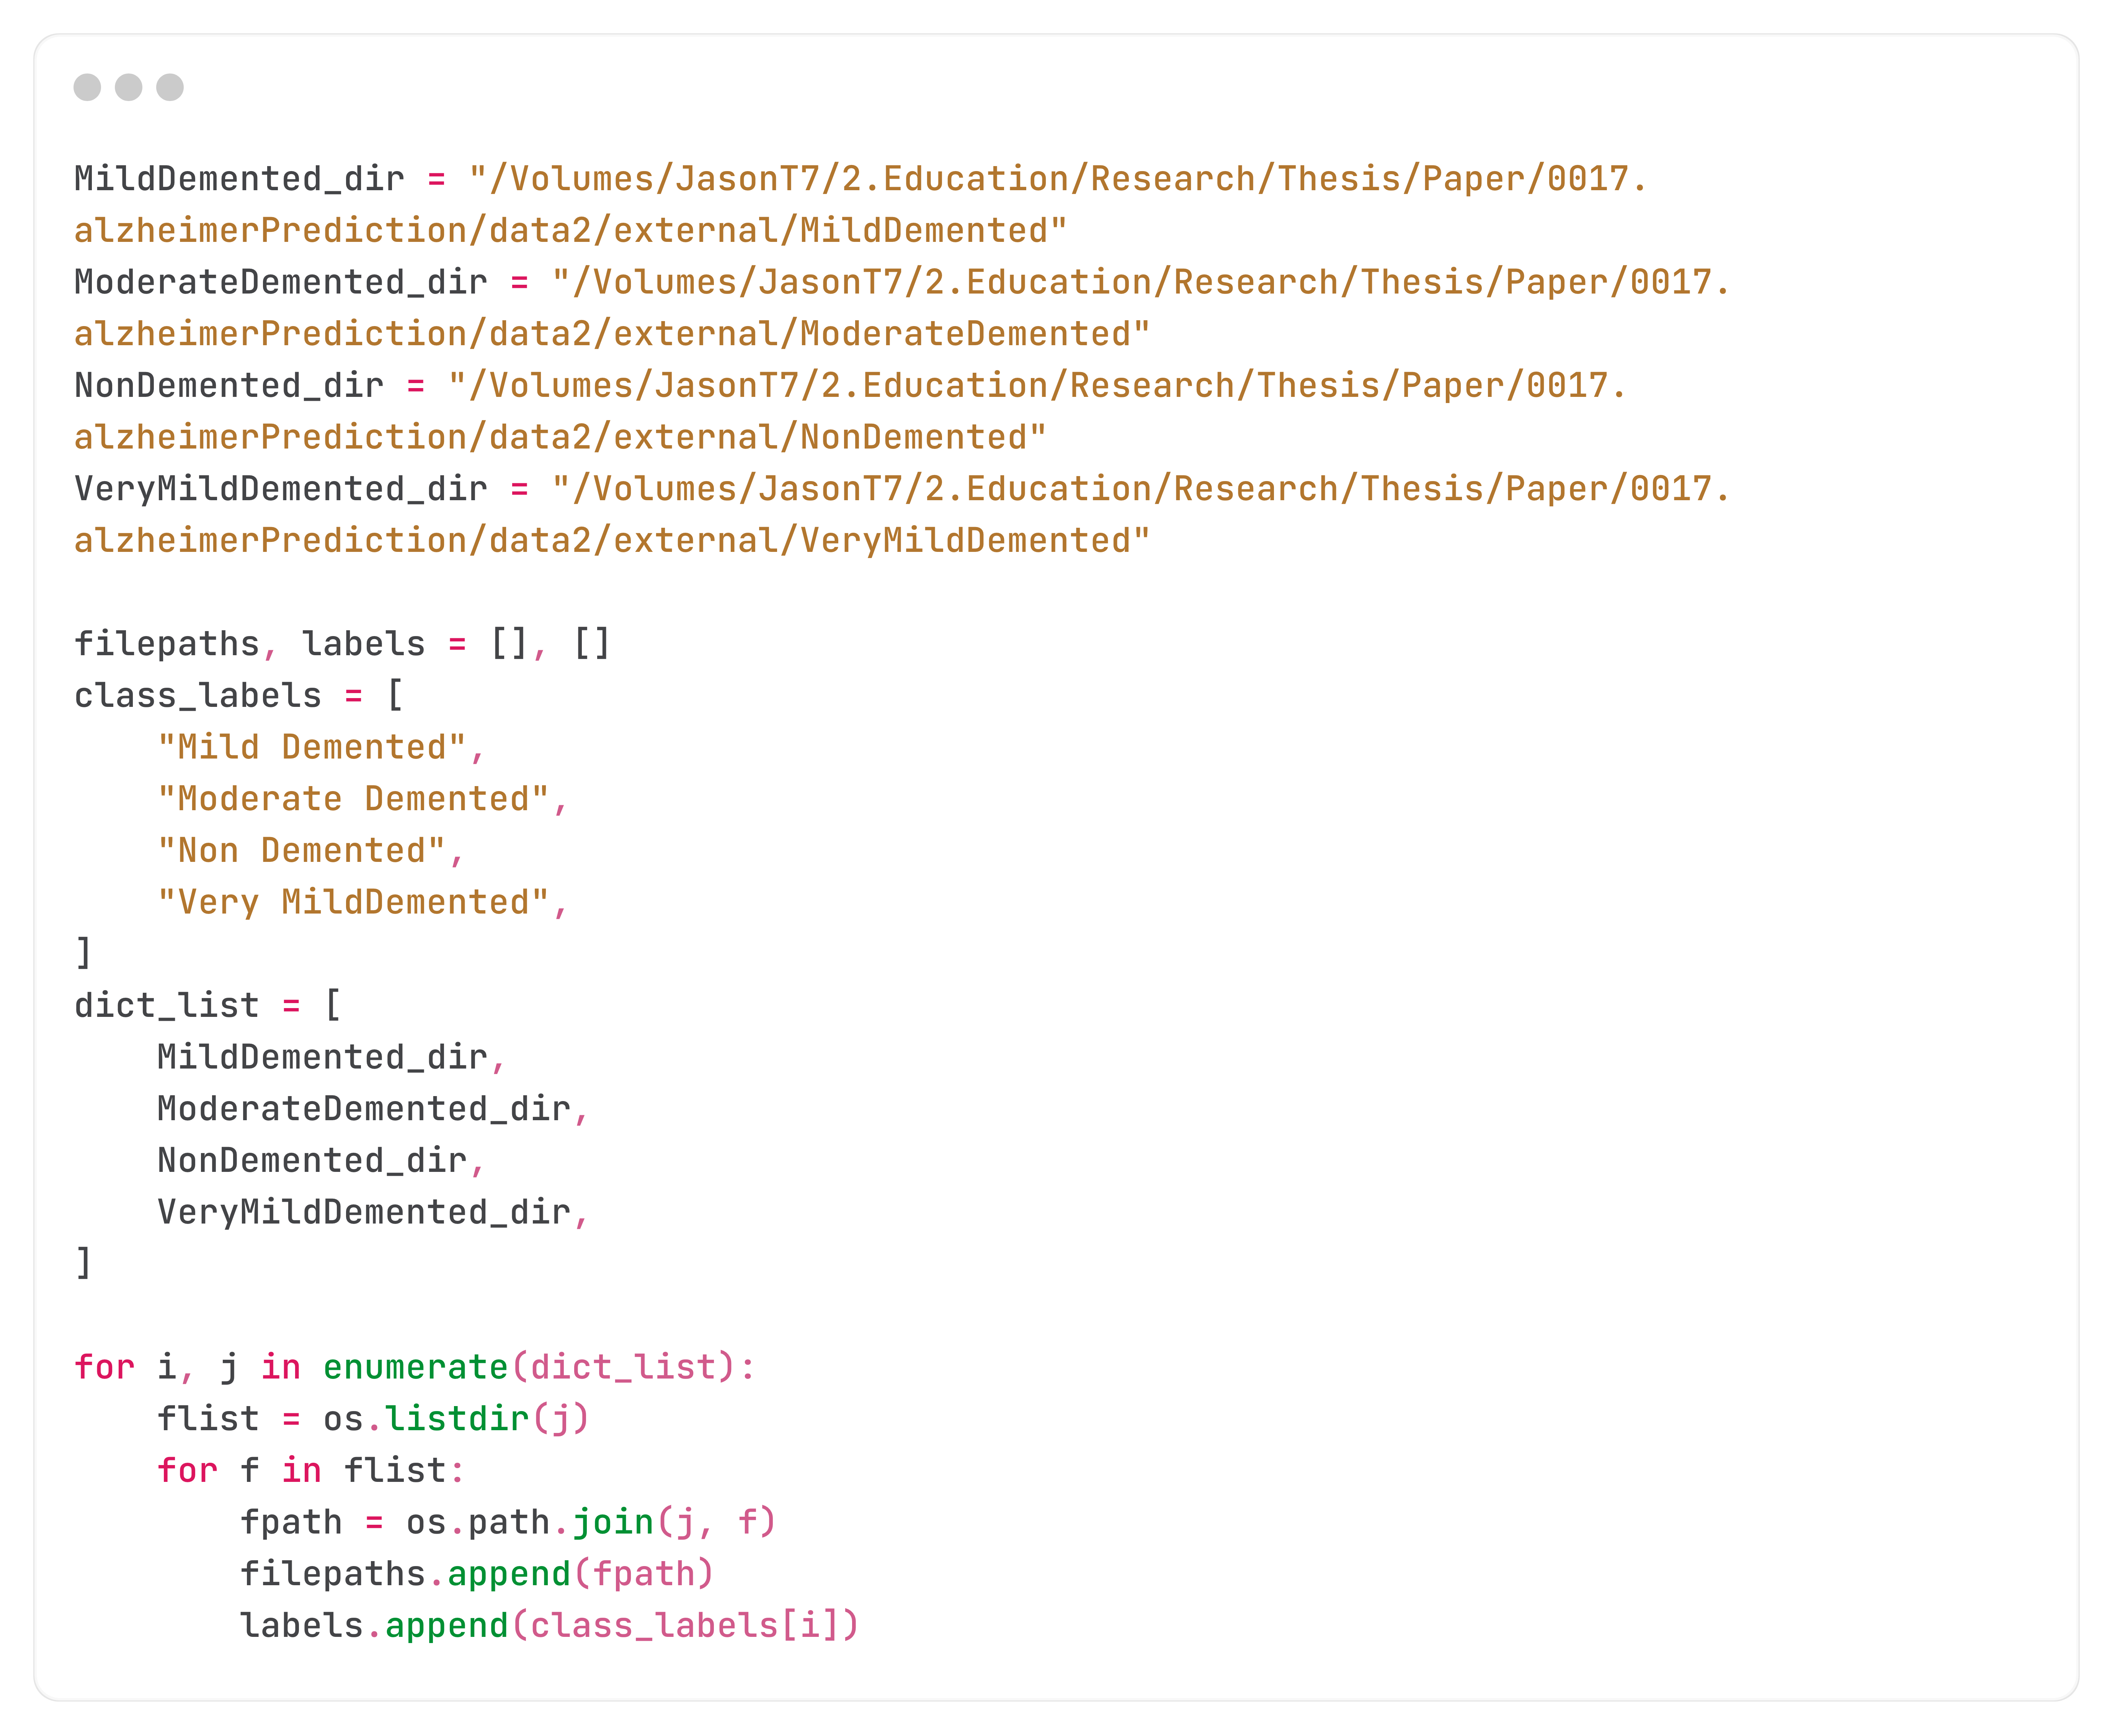
\includegraphics[width=1.0\columnwidth]{figures/loading_images.png}  % Adjust the width to your liking
        \caption{Loading the image paths into a dataset} % Caption for the image
        \label{fig:loading image paths a dataset} % Label to reference the image later in the document
    \end{figure}
    In order to organize and label MRI image data associated with Alzheimer's disease, the given code segment is an essential component of data preparation for a machine learning assignment. It starts by specifying the directory paths for four different types of images: Very Mild Demented, Moderate Demented, Non-Demented, and Mild Demented. Unambiguous access to the data stored in the filesystem is ensured by the absolute paths used to specify these directories.

    The MRI scans in each directory correspond to the associated categorization, which makes supervised learning easier by matching each image to the appropriate label. Next, two empty lists, \texttt{filepaths} and \texttt{labels}, are created. These lists were created to hold the full paths of all image files and the class labels that the images belong to. Additionally, it creates a list called \texttt{class\_labels} that will store the class names for each Alzheimer's disease category that are present in our dataset. This list keeps a relationship in the code by acting as a mapping to the class labels and the path. In order for the script to cycle over the directories in an organized way, a list called \texttt{dict\_list} is simultaneously formed that will store the directory paths.

    A nested loop structure is used for achieving the main functionality. The outer loop uses an enumeration to loop through the \texttt{dict\_list}, where \texttt{i} refers to the image paths's index and \texttt{j} is the image path. This code stores the names of all the files in the current folder after retrieving the list of filenames for each directory using the \texttt{os.listdir()} method. Each file in this list is processed by an inner loop, which uses \texttt{os.path.join()} to add the directory path that is \texttt{j} and the filename that is \texttt{f} to create the file's complete path.

    The proper class labels, obtained from the \texttt{class\_labels} list using the index \texttt{i}, is added to the \texttt{labels} list, and these complete file paths are appended to the \texttt{filepaths} list. The organized dataset that this code creates, where each image corresponds to its proper class name, allows the machine learning model to differentiate between the different stages of Alzheimer's disease. By keeping separate lists of file locations and labels, the code makes sure that the data is ready for further procedures like data splitting, preprocessing, and input into the learning method. Additionally, because it uses directory-specific processing and relative indexing, this method is adaptable and scalable for datasets with similar structures. Further, this integrated method for dataset preparation enables efficient handling of huge, complex data and improves reproducibility.
    \item \textbf{Validation the images using File Path}: 
    \begin{figure}[h!]
        \centering
        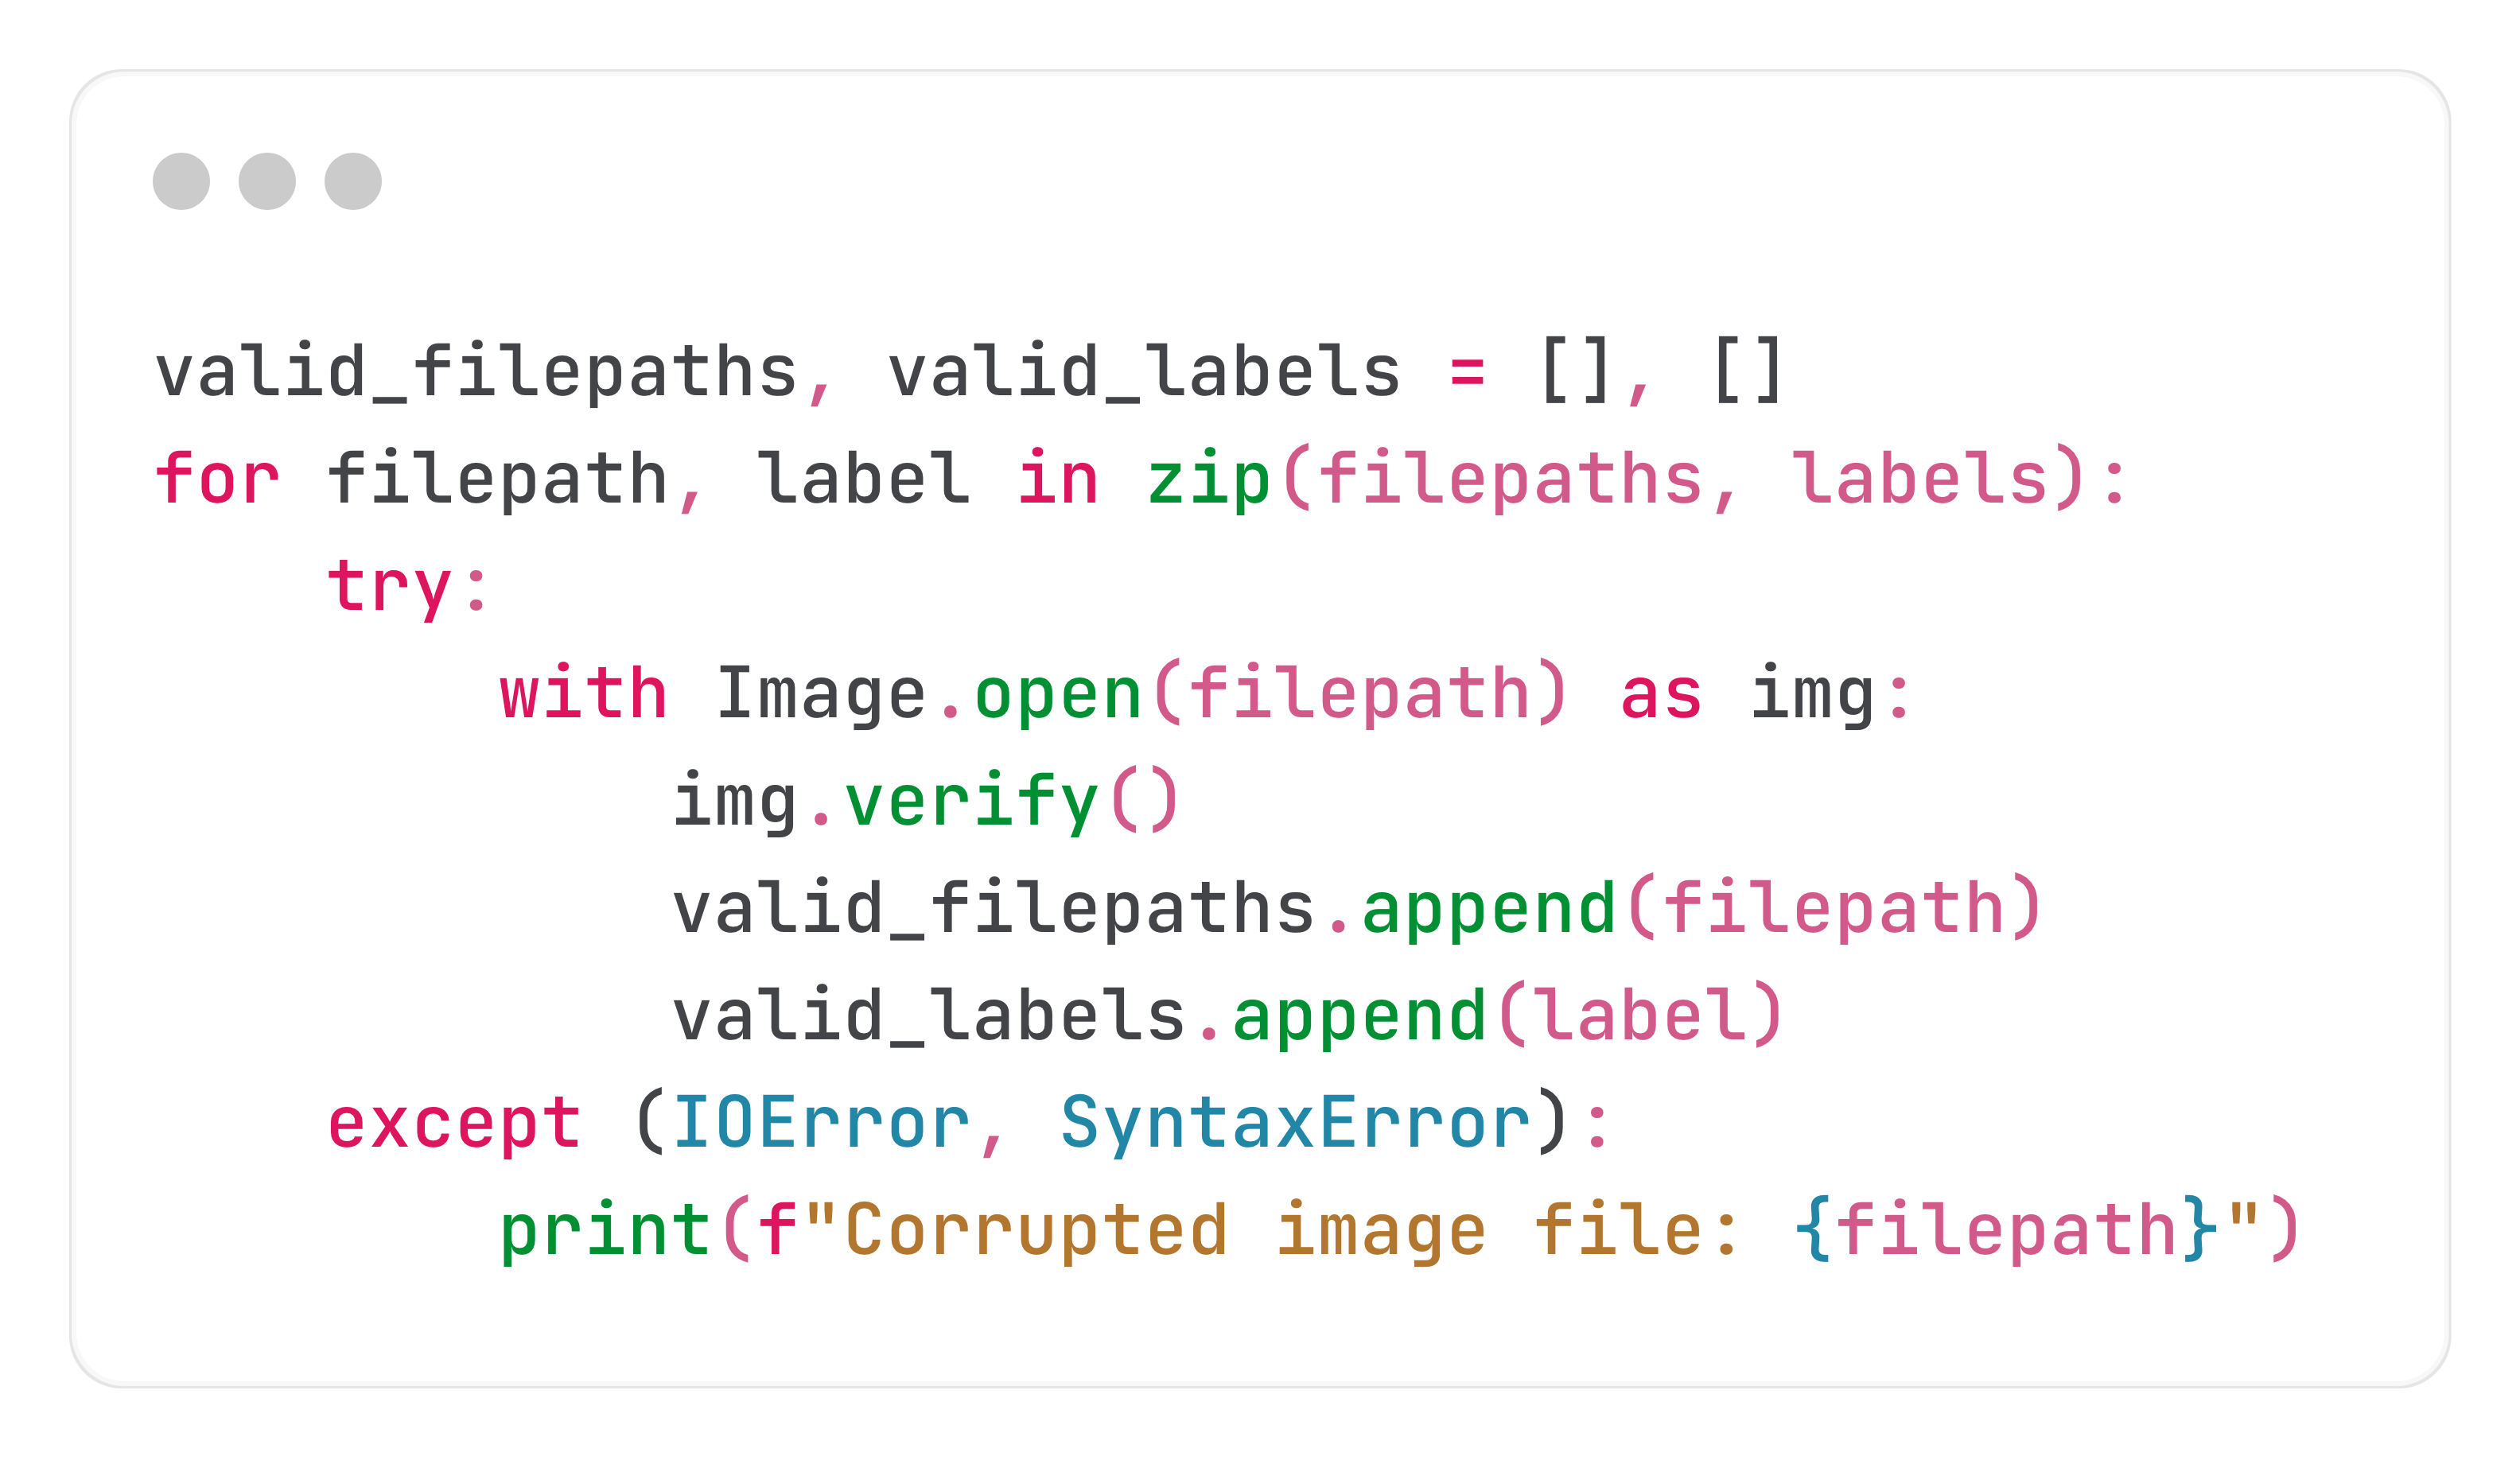
\includegraphics[width=0.6\columnwidth]{figures/validating_images.png}  % Adjust the width to your liking
        \caption{code for validate the images} % Caption for the image
        \label{fig:validating_the_image_using_image_paths} % Label to reference the image later in the document
    \end{figure}
    The \ref{fig:validating_the_image_using_image_paths} shows the code for the preprocessing step meant to make sure that only valid, uncorrupted images files are included in an array of image files and the labels which belong to them. It works by continuously iterating through the lists of \texttt{filepaths} and \texttt{labels}, where each \texttt{filepath} is an image file's disk location and the \texttt{label} is the class or category that goes with it. The \texttt{Image.open(filepath)} function will attempt to try to open each image file that is given by filepath within the loop. The \texttt{img.verify()} method, which checks the image file's validity without fully decoding it. The code adds the image file's path into the \texttt{valid\_filepaths} list and the correct label to the \texttt{valid\_labels} list if the image file is legitimate. The final list will have \texttt{filepaths} and \texttt{labels} for the images that are valid only.

    The code will use the except block to catch any errors that arise in this procedure, whether they are caused by damaged, unreadable, or invalid file formats. Particularly, the code deals with two exceptions: \texttt{SyntaxError}, which may be raised if the file is incorrectly written as an image, and \texttt{IOError}, which usually happens when a file cannot be read. By using this method, it is ensured that corrupted files won't interfere with further processing steps or model training, which might otherwise end up in mistakes or lower dataset quality. 
    \item \textbf{Dividing the data}:
    \begin{figure}[h!]
        \centering
        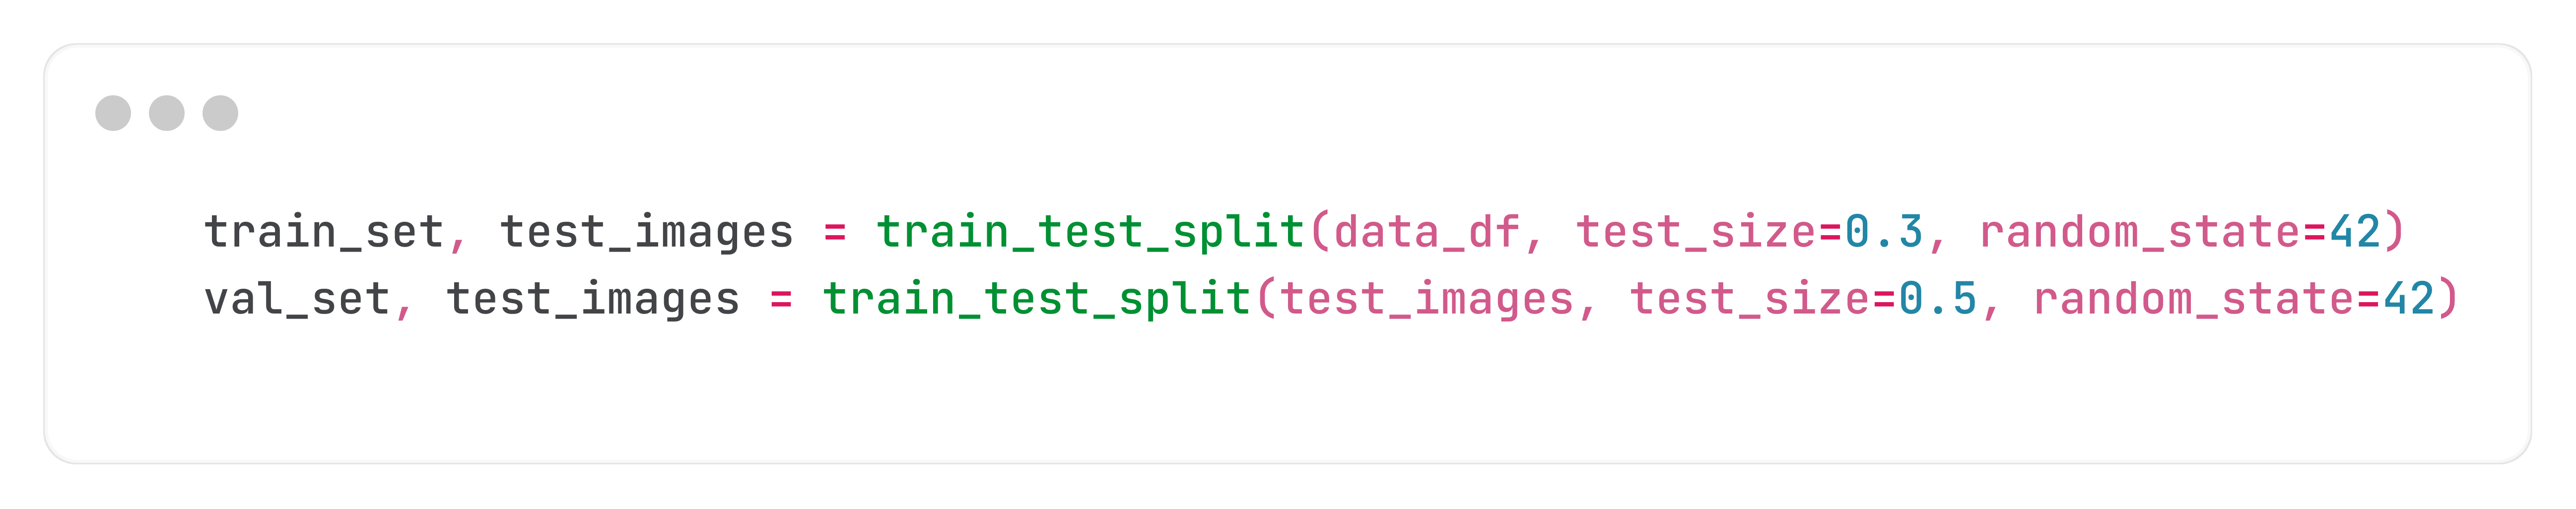
\includegraphics[width=0.9\columnwidth]{figures/data_spliting.png}  % Adjust the width to your liking
        \caption{code for dividing the dataset} % Caption for the image
        \label{fig:dividing_the_dataset} % Label to reference the
    \end{figure}
    Figure \ref{fig:dividing_the_dataset} shows the code snippet for having the dataset ready for training, validation, and testing. It makes use of the \texttt{sklearn.model\_selection} module's \texttt{train\_test\_split} function to divide datasets into three dataframes that is test, train and validation. The dataset, denoted by \texttt{data\_df}, is divided into two halves in the first line, a temporary test set (\texttt{test\_images}) and a training set (\texttt{train\_set}). 30\% of the dataset is allotted to the test set, with the remaining 70\% left aside for training, according to the \texttt{test\_size}=0.3 option. The reproducibility of the splitting operation is guaranteed by the setting \texttt{random\_state}=42.The second line splits the temporary test set (\texttt{test\_images}) into two equal parts, a final test set  and a validation set (\texttt{val\_set}). The code makes sure that the temporary test set is divided equally by assigning 50\% of its data to each subgroup by setting \texttt{test\_size=0.5}. To keep the splitting procedure consistent, the \texttt{random\_state=42} argument is again used.
    \item \textbf{Preprocessing the Images}:
    \begin{figure}[h!]
        \centering
        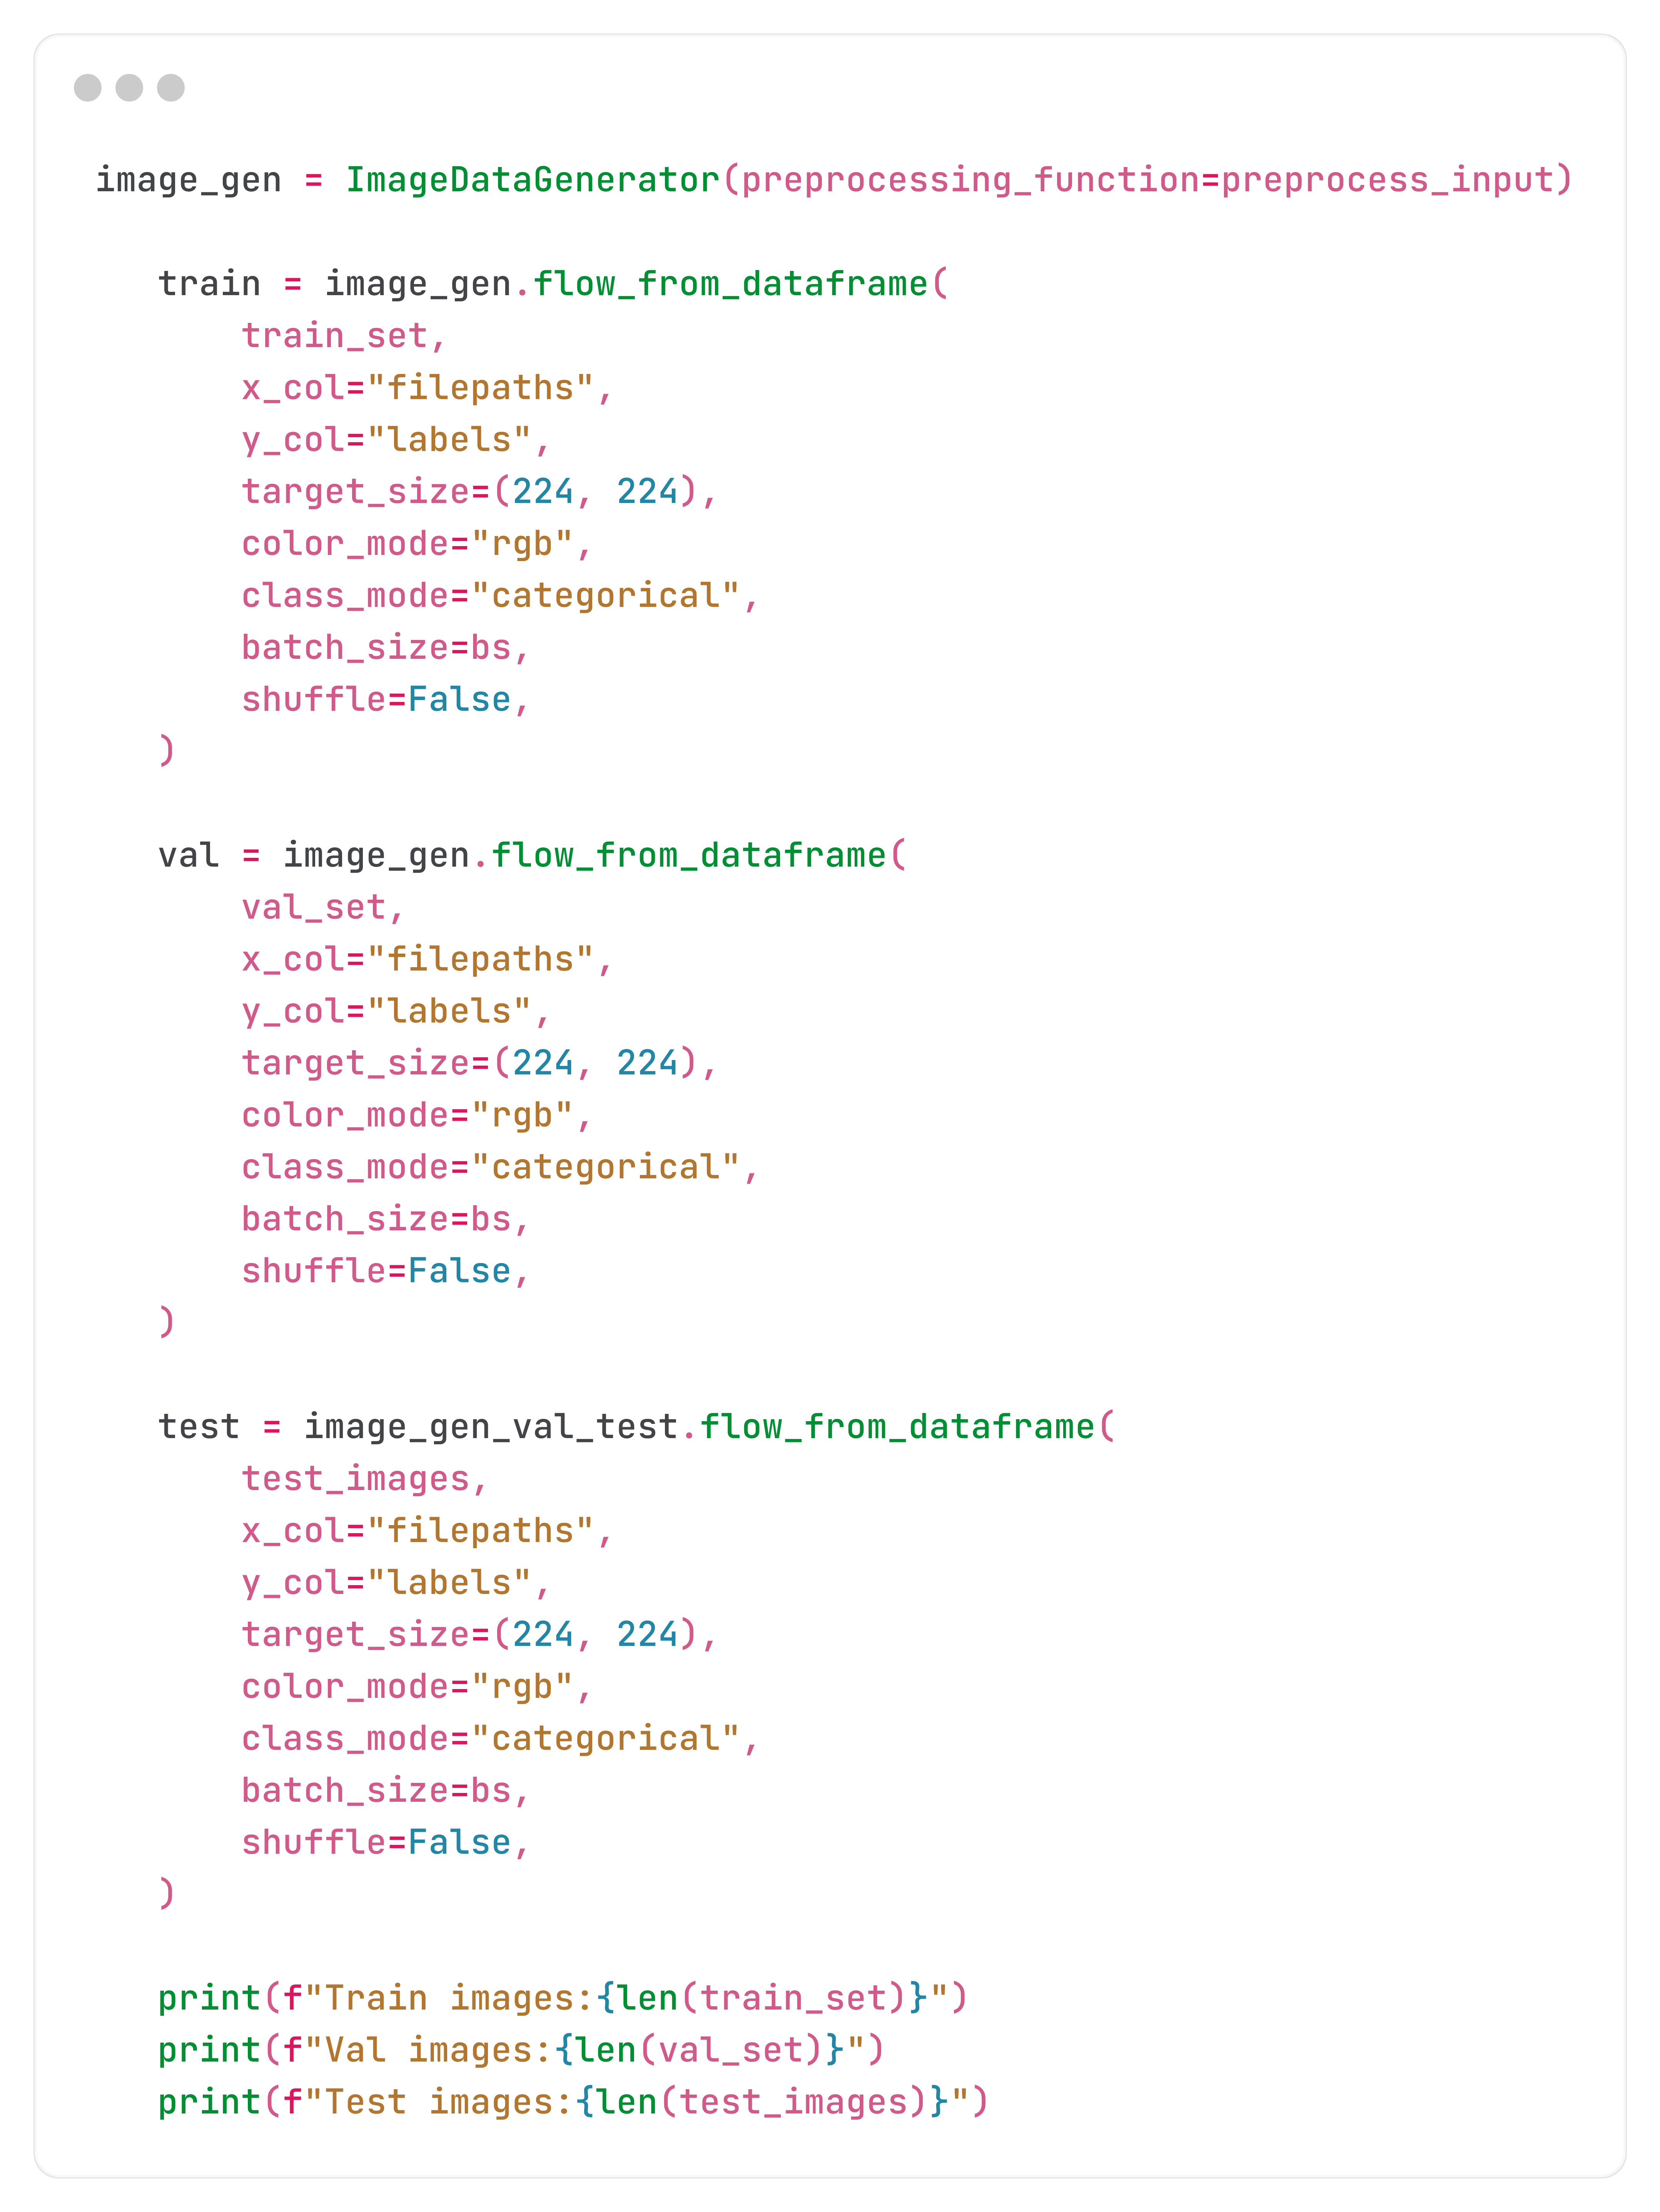
\includegraphics[width=0.6\columnwidth]{figures/imp_data_preprocessing.png}  % Adjust the width to your liking
        \caption{code for image data pre-processing} % Caption for the image
        \label{fig:imp_data_preprocessing} % Label to reference the
    \end{figure}
    This is an important step for getting the picture datasets set up for training, validation, and testing with \texttt{Keras'} \texttt{ImageDataGenerator} class. The figure \ref{fig:imp_data_preprocessing} shows the code for pre-processing. Image Data Generator is a component of the \texttt{TensorFlow} library. It guarantees that the information is correctly organized and preprocessed before being fed into a convolutional neural network. For the training data (\texttt{image\_gen\_train}) and the validation and test datasets (\texttt{image\_gen\_val\_test}), \texttt{ImageDataGenerator} is generated. The preprocessing function \texttt{preprocess\_input}, which is utilized by the generators, standardizes the input photos in accordance with the expected specifications of the \texttt{Effici\newline entNetB0} model. 

    The training, validation, and testing datasets are then loaded and preprocessed using the \texttt{flow\_from\_dataf\newline rame} function. It resizes photos to 224x224 pixels, formats them as \texttt{RGB}, applies categorical labels for a multi-class classification task, and extracts image paths and labels from the corresponding dataframes (\texttt{train\_set}, \texttt{val\_set}, \texttt{test\_images}). The number of photos processed in each batch is determined by the \texttt{batch\_size}, and the data order is maintained by using \texttt{shuffle=False}.
    
    For consistency, the same generator is used to process the training and validation datasets, while a different generator (\texttt{image\_gen\_val\_test}) handles the test set, providing flexibility for different preprocessing if necessary. Every dataset preserves consistent transformations, guaranteeing that the model assesses performance in a consistent manner.
\end{itemize}

\subsection{Model Development}
\begin{figure}[H]
    \centering
    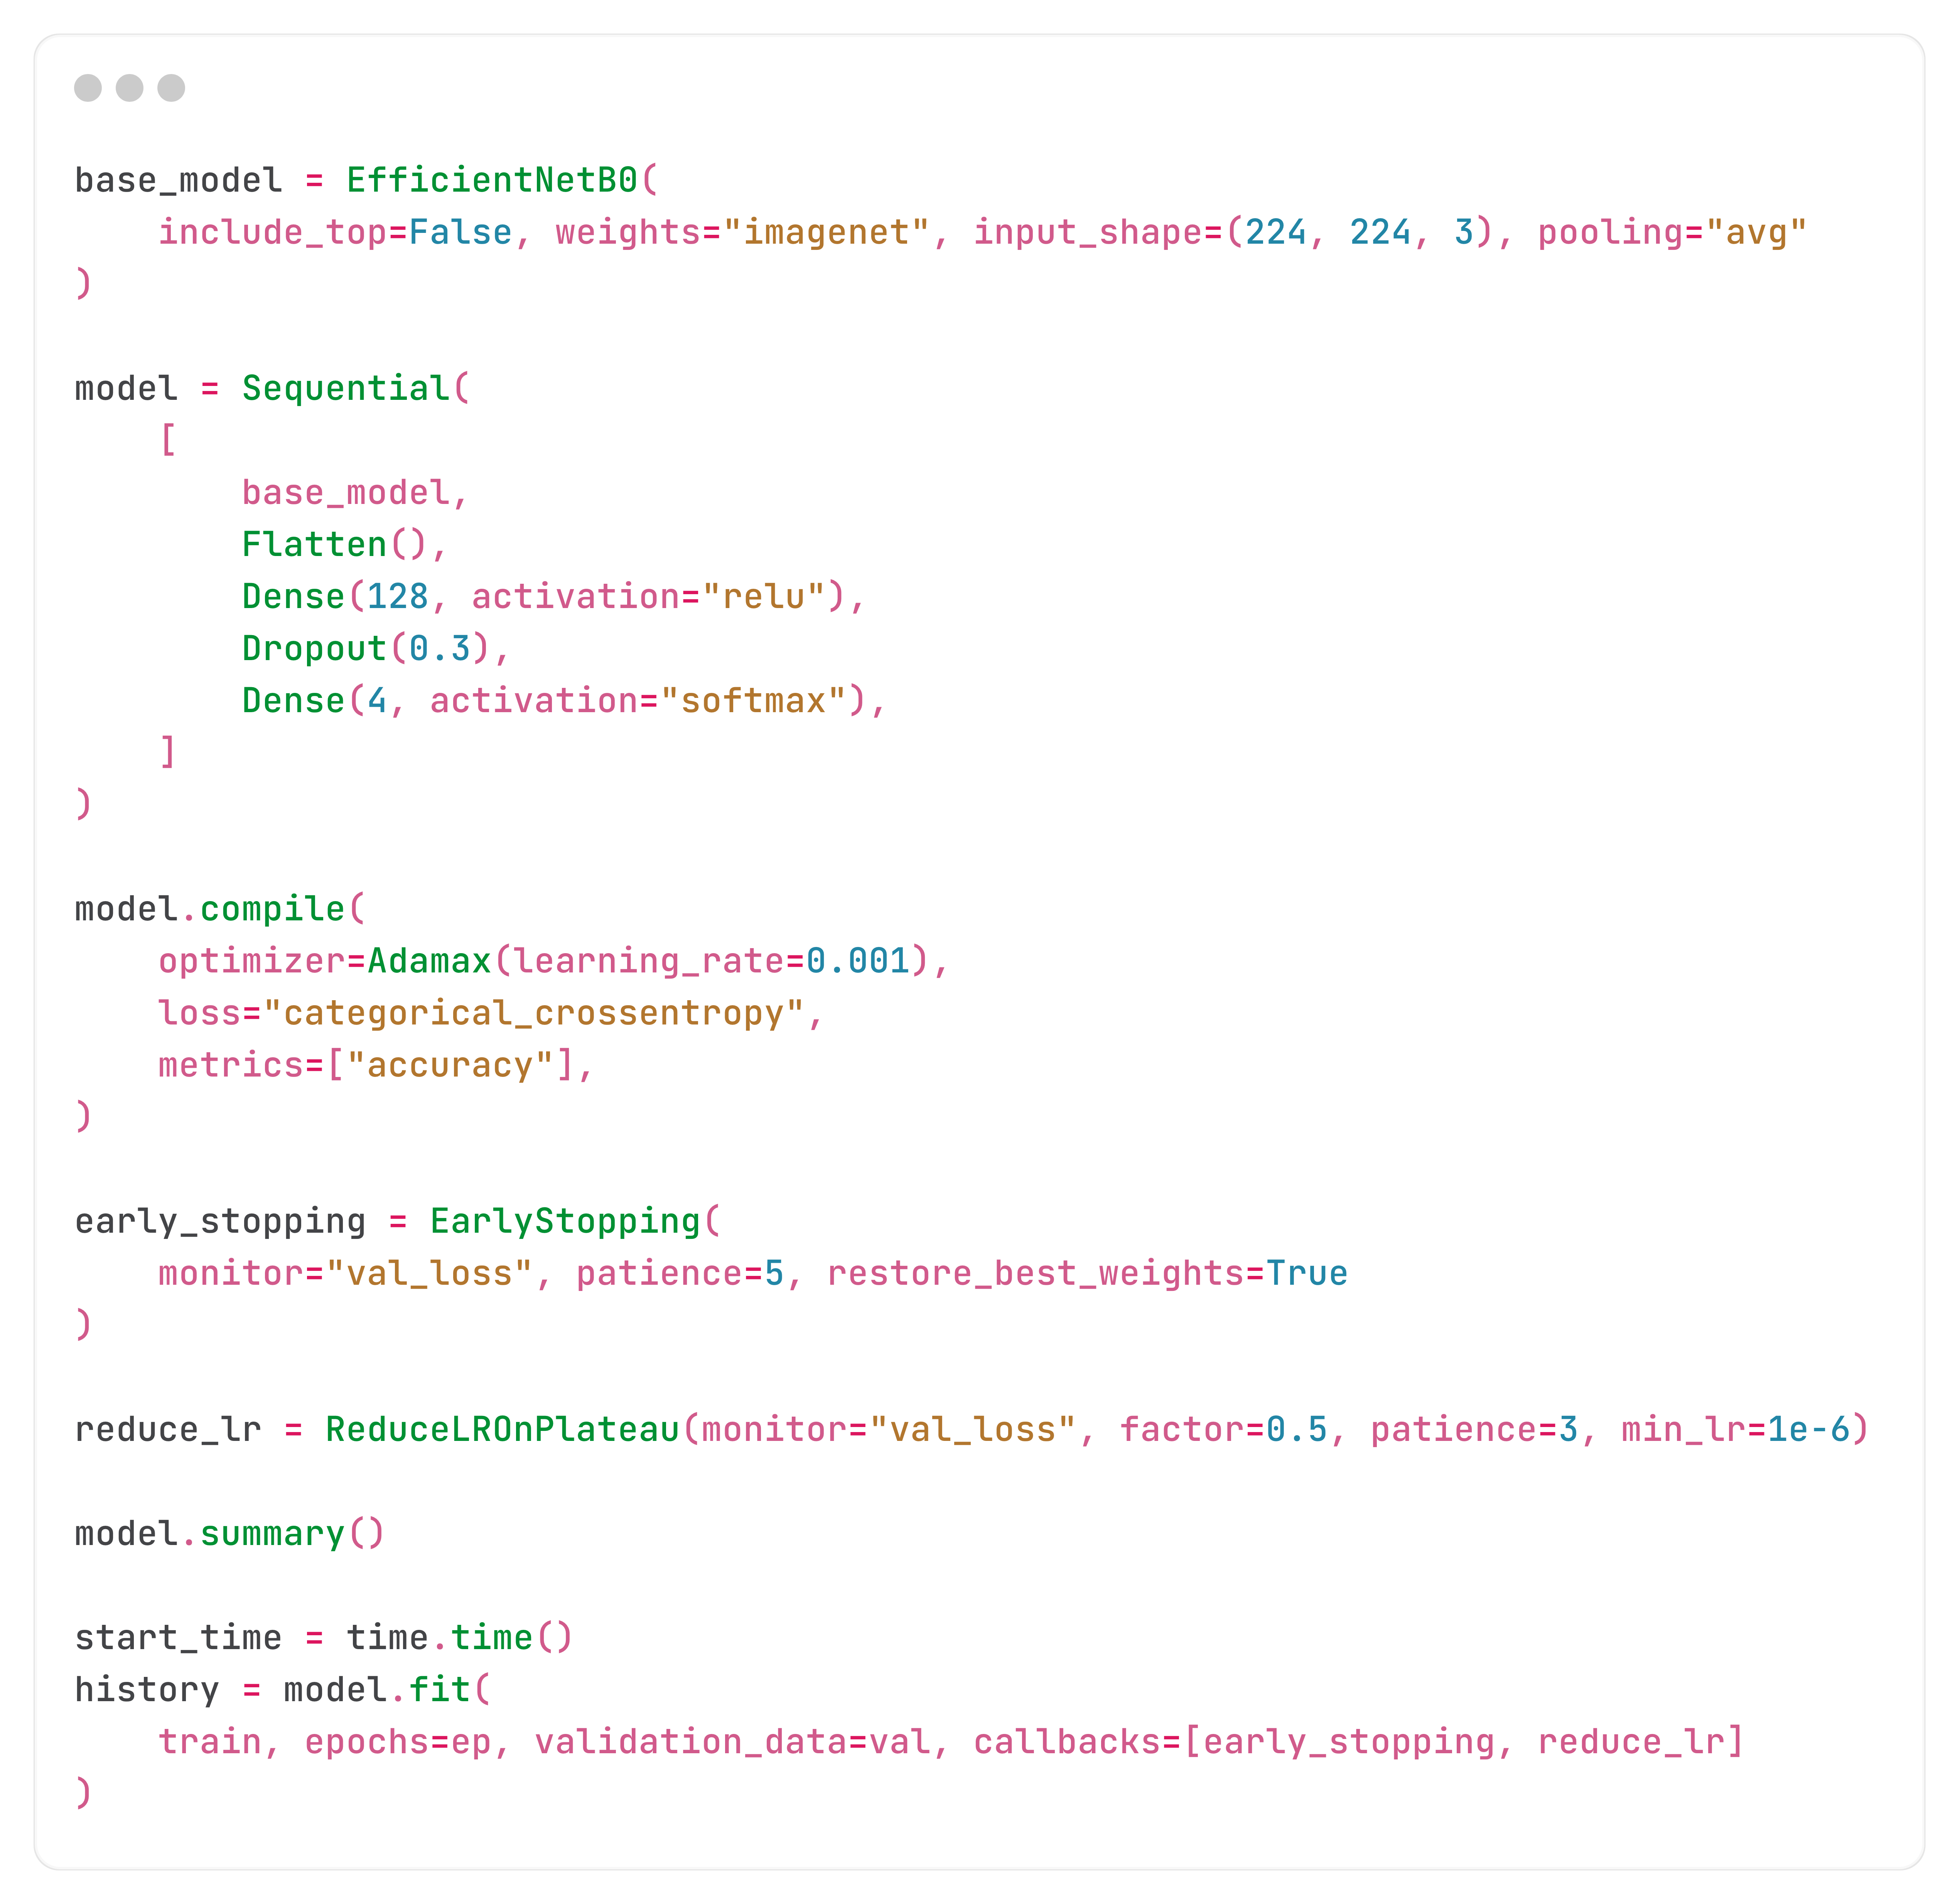
\includegraphics[width=0.8\columnwidth]{figures/imp_model_training.png}  % Adjust the width to your liking
    \caption{code for model training} % Caption for the image
    \label{fig:imp_model_training} % Label to reference the
\end{figure}
\subsubsection{Base model}
\texttt{EfficientNetB0}, a pretrained model, is selected as the base model to extract the basic features at the beginning of the process. \texttt{EfficientNetB0} is an advanced convolutional neural network that was trained on the dataset from \texttt{ImageNet}. It is known for its effectiveness and strong performance on a range of uses. The pretrained model's top classification layer is excluded by setting \texttt{include\_top=False}, enabling customization for the task at hand. \texttt{Pooling="avg"} uses global average pooling to lower the dimensionality of the output from the convolutional layers, while the \texttt{input\_shape} parameter sets the size of the input images to ensure network compatibility. Pretrained weights from \texttt{ImageNet} are included to guarantee that the network makes use of a wealth of characteristics acquired during extensive training, greatly accelerating convergence and enhancing accuracy for the specified dataset.



\subsubsection{Training the Model and Optimizing}
The base model is then easily customized and made more adaptable by integrating it into a \texttt{Sequential} model, which is a linear stack of layers in \texttt{Keras}. The output is flattened using the \texttt{Flatten()} layer after the base model, which transforms the multidimensional tensor into a one-dimensional vector appropriate for the dense layers. The addition of a \texttt{Dense} layer with 128 units and \texttt{ReLU} activation creates a fully connected layer that can recognize intricate patterns in the data. A \texttt{Dropout} layer with a rate of 0.3 is incorporated to lessen overfitting. During training, 30\% of the weights are randomly set to zero. The last layer, another \texttt{Dense} layer, uses a \texttt{softmax} activation function to output class probabilities and has four units, which correspond to the number of output classes.
The \texttt{Adamax} optimizer is an adaptive learning rate optimization method that was inspired by \texttt{Adam}. \texttt{Adamax} is used to construct the model. It is set up with a learning rate of 0.001 and is especially good at managing sparse gradients. \texttt{Accuracy}, which measures the percentage of accurate predictions, is the evaluation metric. The loss function is set to \texttt{categorical\_crossentropy}, a common option for multi-class classification tasks.

Two callbacks, \texttt{EarlyStopping} and \texttt{ReduceLROnPlateau}, are used to improve training efficiency and avoid overfitting. The \texttt{EarlyStopping} callback restores the optimal weights seen during training by tracking the validation loss (\texttt{val\_loss}) and stopping training if there is no improvement for five consecutive epochs. With a minimum learning rate threshold of \(1 \times 10^{-6}\), the \texttt{ReduceLROnPlateau} callback automatically lowers the learning rate by a factor of 0.5 if the validation loss does not improve after three epochs. By avoiding needless training epochs, these callbacks guarantee that the model converges efficiently.

And then a summary of the model is generated. The \texttt{fit} method, which starts training, requires three inputs: the validation dataset (\texttt{val}), the number of epochs (\texttt{ep}), and the training dataset (\texttt{train}). To ensure no dynamic changes during training, the callbacks are provided as a list. The training duration is measured using the \texttt{time.time()} method, which offers information about the model's computational effectiveness. To attain the best results in multi-class image classification jobs, this end-to-end configuration incorporates cutting-edge methods and resources.

\subsection{Adding Uncertainity estimation to the mix}
\begin{figure}[H]
    \centering
    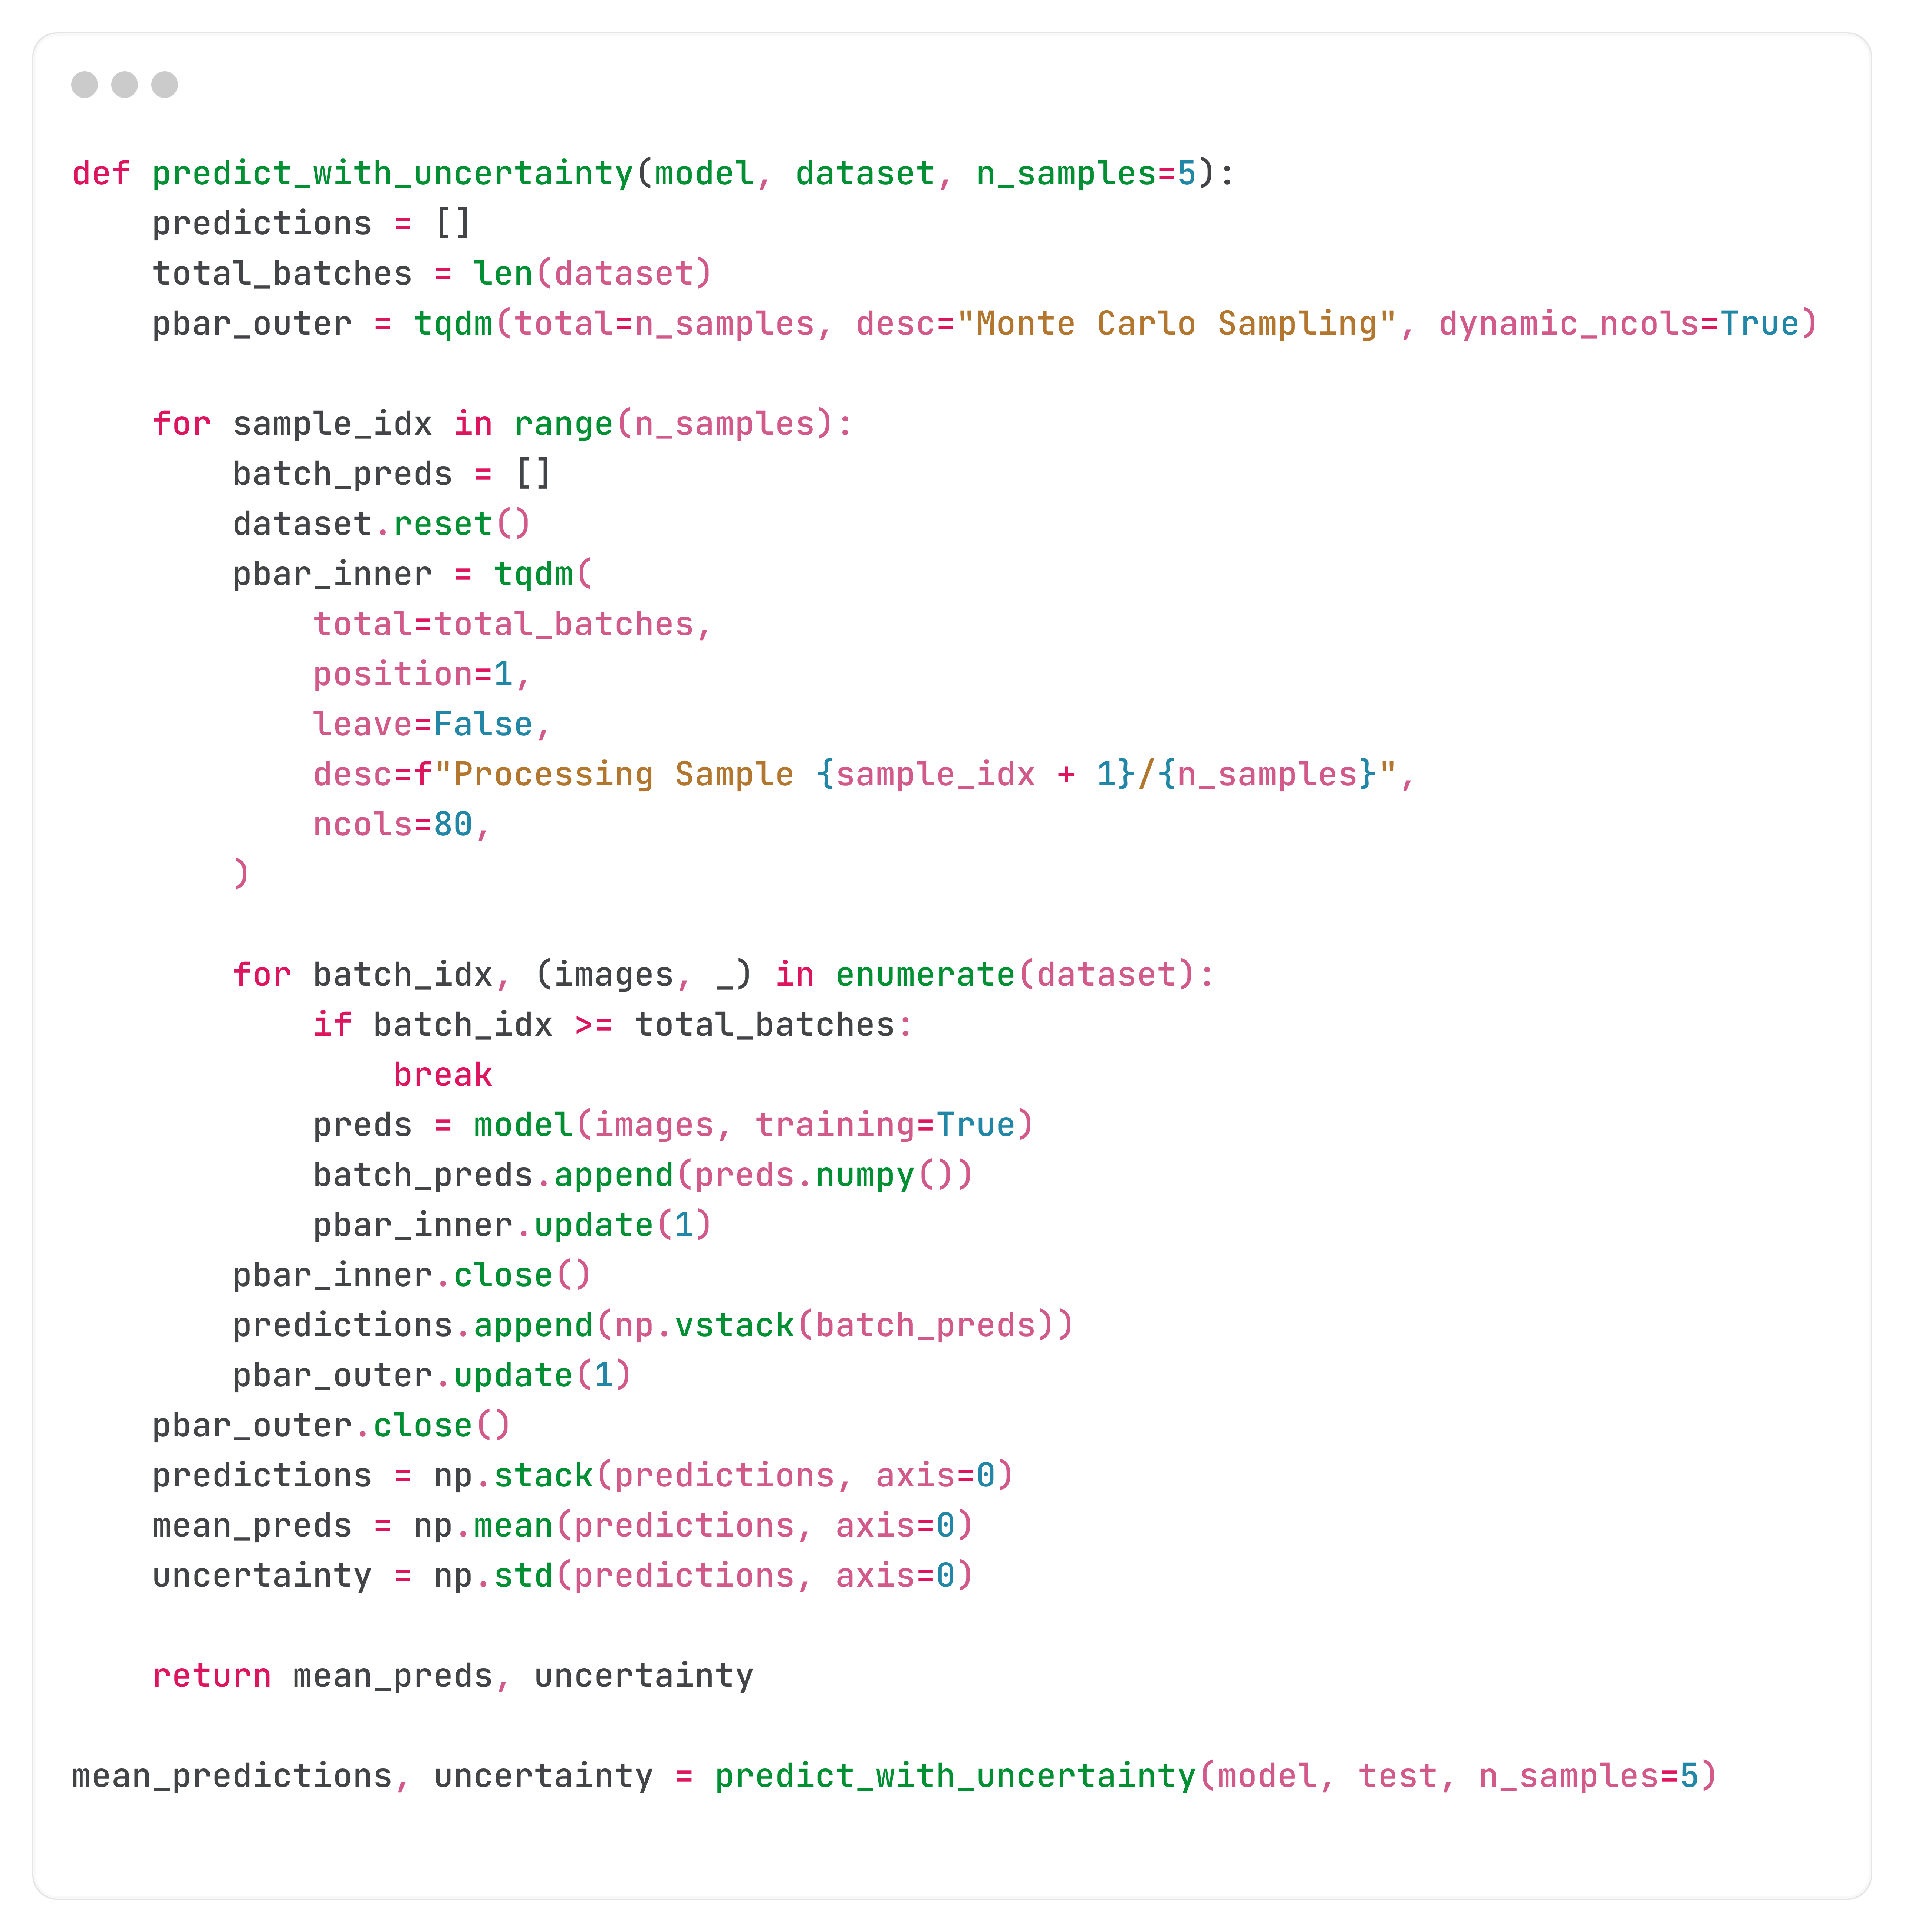
\includegraphics[width=0.8\columnwidth]{figures/imp_uncertainity_estimation.png}  % Adjust the width to your liking
    \caption{code for uncertainity estimation} % Caption for the image
    \label{fig:imp_uncertainity_estimation} % Label to reference the
\end{figure}
This code uses \texttt{Monte Carlo dropout} sampling for calculating uncertainty. It is a \texttt{Bayesian} technique that takes into account model prediction variability based on the random nature of \texttt{dropout} layers, to evaluate predictive uncertainty. To measure uncertainty, the \texttt{predict\_with\_uncertainty} function does multiple forward tests with the model in training mode even during inference. This function needs three inputs: the number of \texttt{MC} samples (\texttt{n\_samples}), a dataset (usually for testing), and the trained model. It determines the total number of batches in the dataset and initializes an empty list called \texttt{predictions} to hold the outcomes of several forward runs. Throughout the designated number of iterations, the sampling process is tracked via a progress bar (\texttt{pbar\_outer}).

To make sure of consistent processing, the dataset is reset after every \texttt{MC} sample, and batch-wise progress is monitored by a separate progress bar (\texttt{pbar\_inner}). The model adds predictions to \texttt{batch\_preds} as \texttt{NumPy} arrays while processing batches of photos while maintaining \texttt{dropout} layers active, that is, with \texttt{training=True}. Predictions for the sample are stacked and added to the \texttt{predictions} list once all batches have been processed. For the designated number of samples, this procedure is repeated. \texttt{Predictions} are merged into a three-dimensional array after every sample is finished. Along the sample axis, the function computes the \texttt{standard deviation} (that is, \texttt{uncertainty}) and \texttt{mean predictions} (that is, \texttt{mean\_preds}). The standard deviation measures the degree of uncertainty surrounding the model's final predictions, whereas the mean represents those forecasts.

\subsection{Performance Evaluation}
\begin{figure}[H]
    \centering
    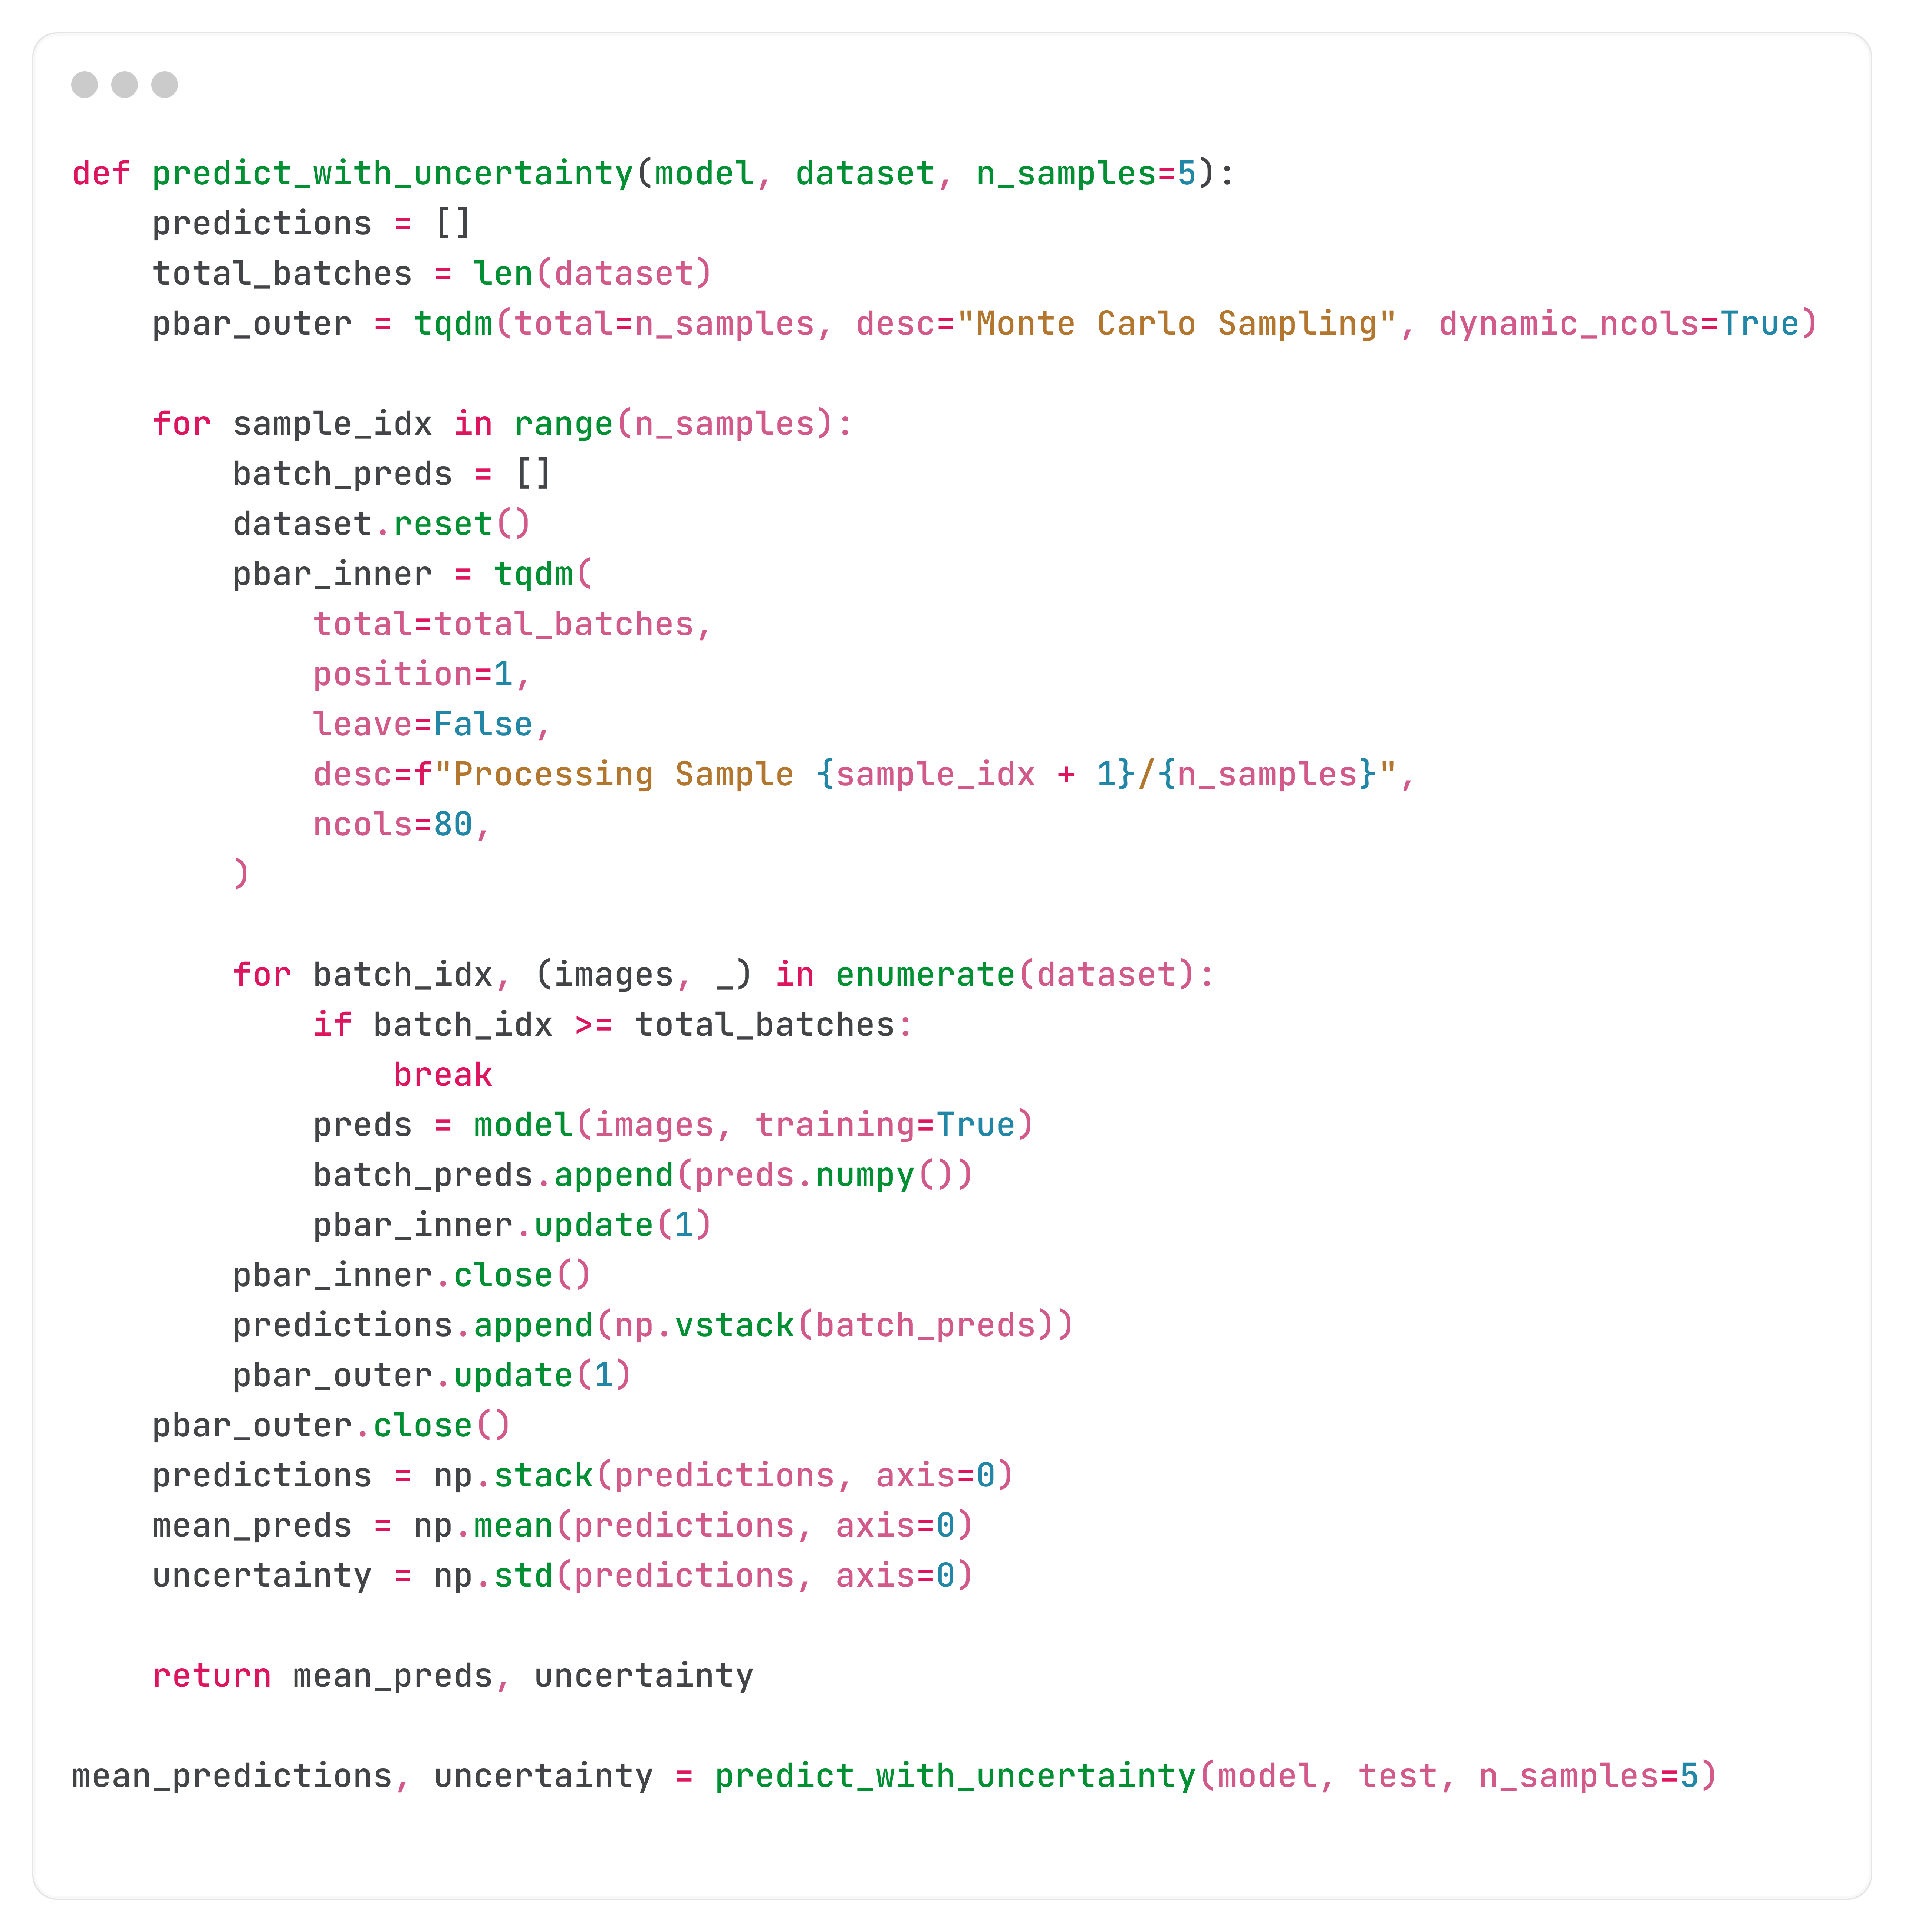
\includegraphics[width=0.8\columnwidth]{figures/imp_uncertainity_estimation.png}  % Adjust the width to your liking
    \caption{code for uncertainity estimation} % Caption for the image
    \label{fig:imp_uncertainity_estimation} % Label to reference the
\end{figure}
This code evaluates a multi-class classification model by calculating metrics and organizing them. It extracts ground truth labels \texttt{y\_true} from the test dataset and converts them into a \texttt{NumPy} array. Predicted labels \texttt{y\_pred} are generated using \texttt{np.argmax} on \texttt{mean\_predictions}. The \texttt{sklearn.metrics} \texttt{classification\_report} function computes precision, recall, and F1-score for each class, linking them to class names with \texttt{target\_names=\newline class\_labels}. The \texttt{output\_dict=True} option returns the report as a dictionary, converted to a \texttt{Pandas DataFrame} \texttt{class\_metrics} for analysis. Class-level accuracies are calculated as correct predictions per class relative to total samples, stored in \texttt{class\_accuracy} and added to \texttt{class\_metrics}. Aggregate accuracy metrics—macro, micro, and weighted averages—are computed for broader evaluation. Precision, recall, and F1-score are also computed for micro-average, stored in the \texttt{"micro avg"} row of \texttt{class\_metrics}. Finally, \texttt{class\_metri\newline cs} \texttt{DataFrame} is displayed, offering a comprehensive breakdown of metrics for each class and overall performance.

\subsection{Integrating the Model with a Web Application}
The model that is trained on these images of MRI multiples classes images will be saved to the directory, and then this model will be used to connect to an web application which makes use of Flask API to upload the image and the predict the images into the class which it belongs to. Python code used to write the backend of this webapplication and a basic html to design the page and the a css is applied on top of this html to style the web application. The Flask framework will make use fo RESTfull API. The Webapplication has two buttons:
\begin{itemize}
    \item \textbf{Upload Button}: The upload button is used to select the images from the local storage. Once it is upload there will be a preview of the image that is being uploaded.
    \item \textbf{Predict Button}: The Predict button will take the user to the prediction screen where the predicted class and the confidence score is calculated and displayed in the progress bar.
\end{itemize}


\subsubsection{Connect the backend with the Flask API Integration}
\begin{figure}[H]
    \centering
    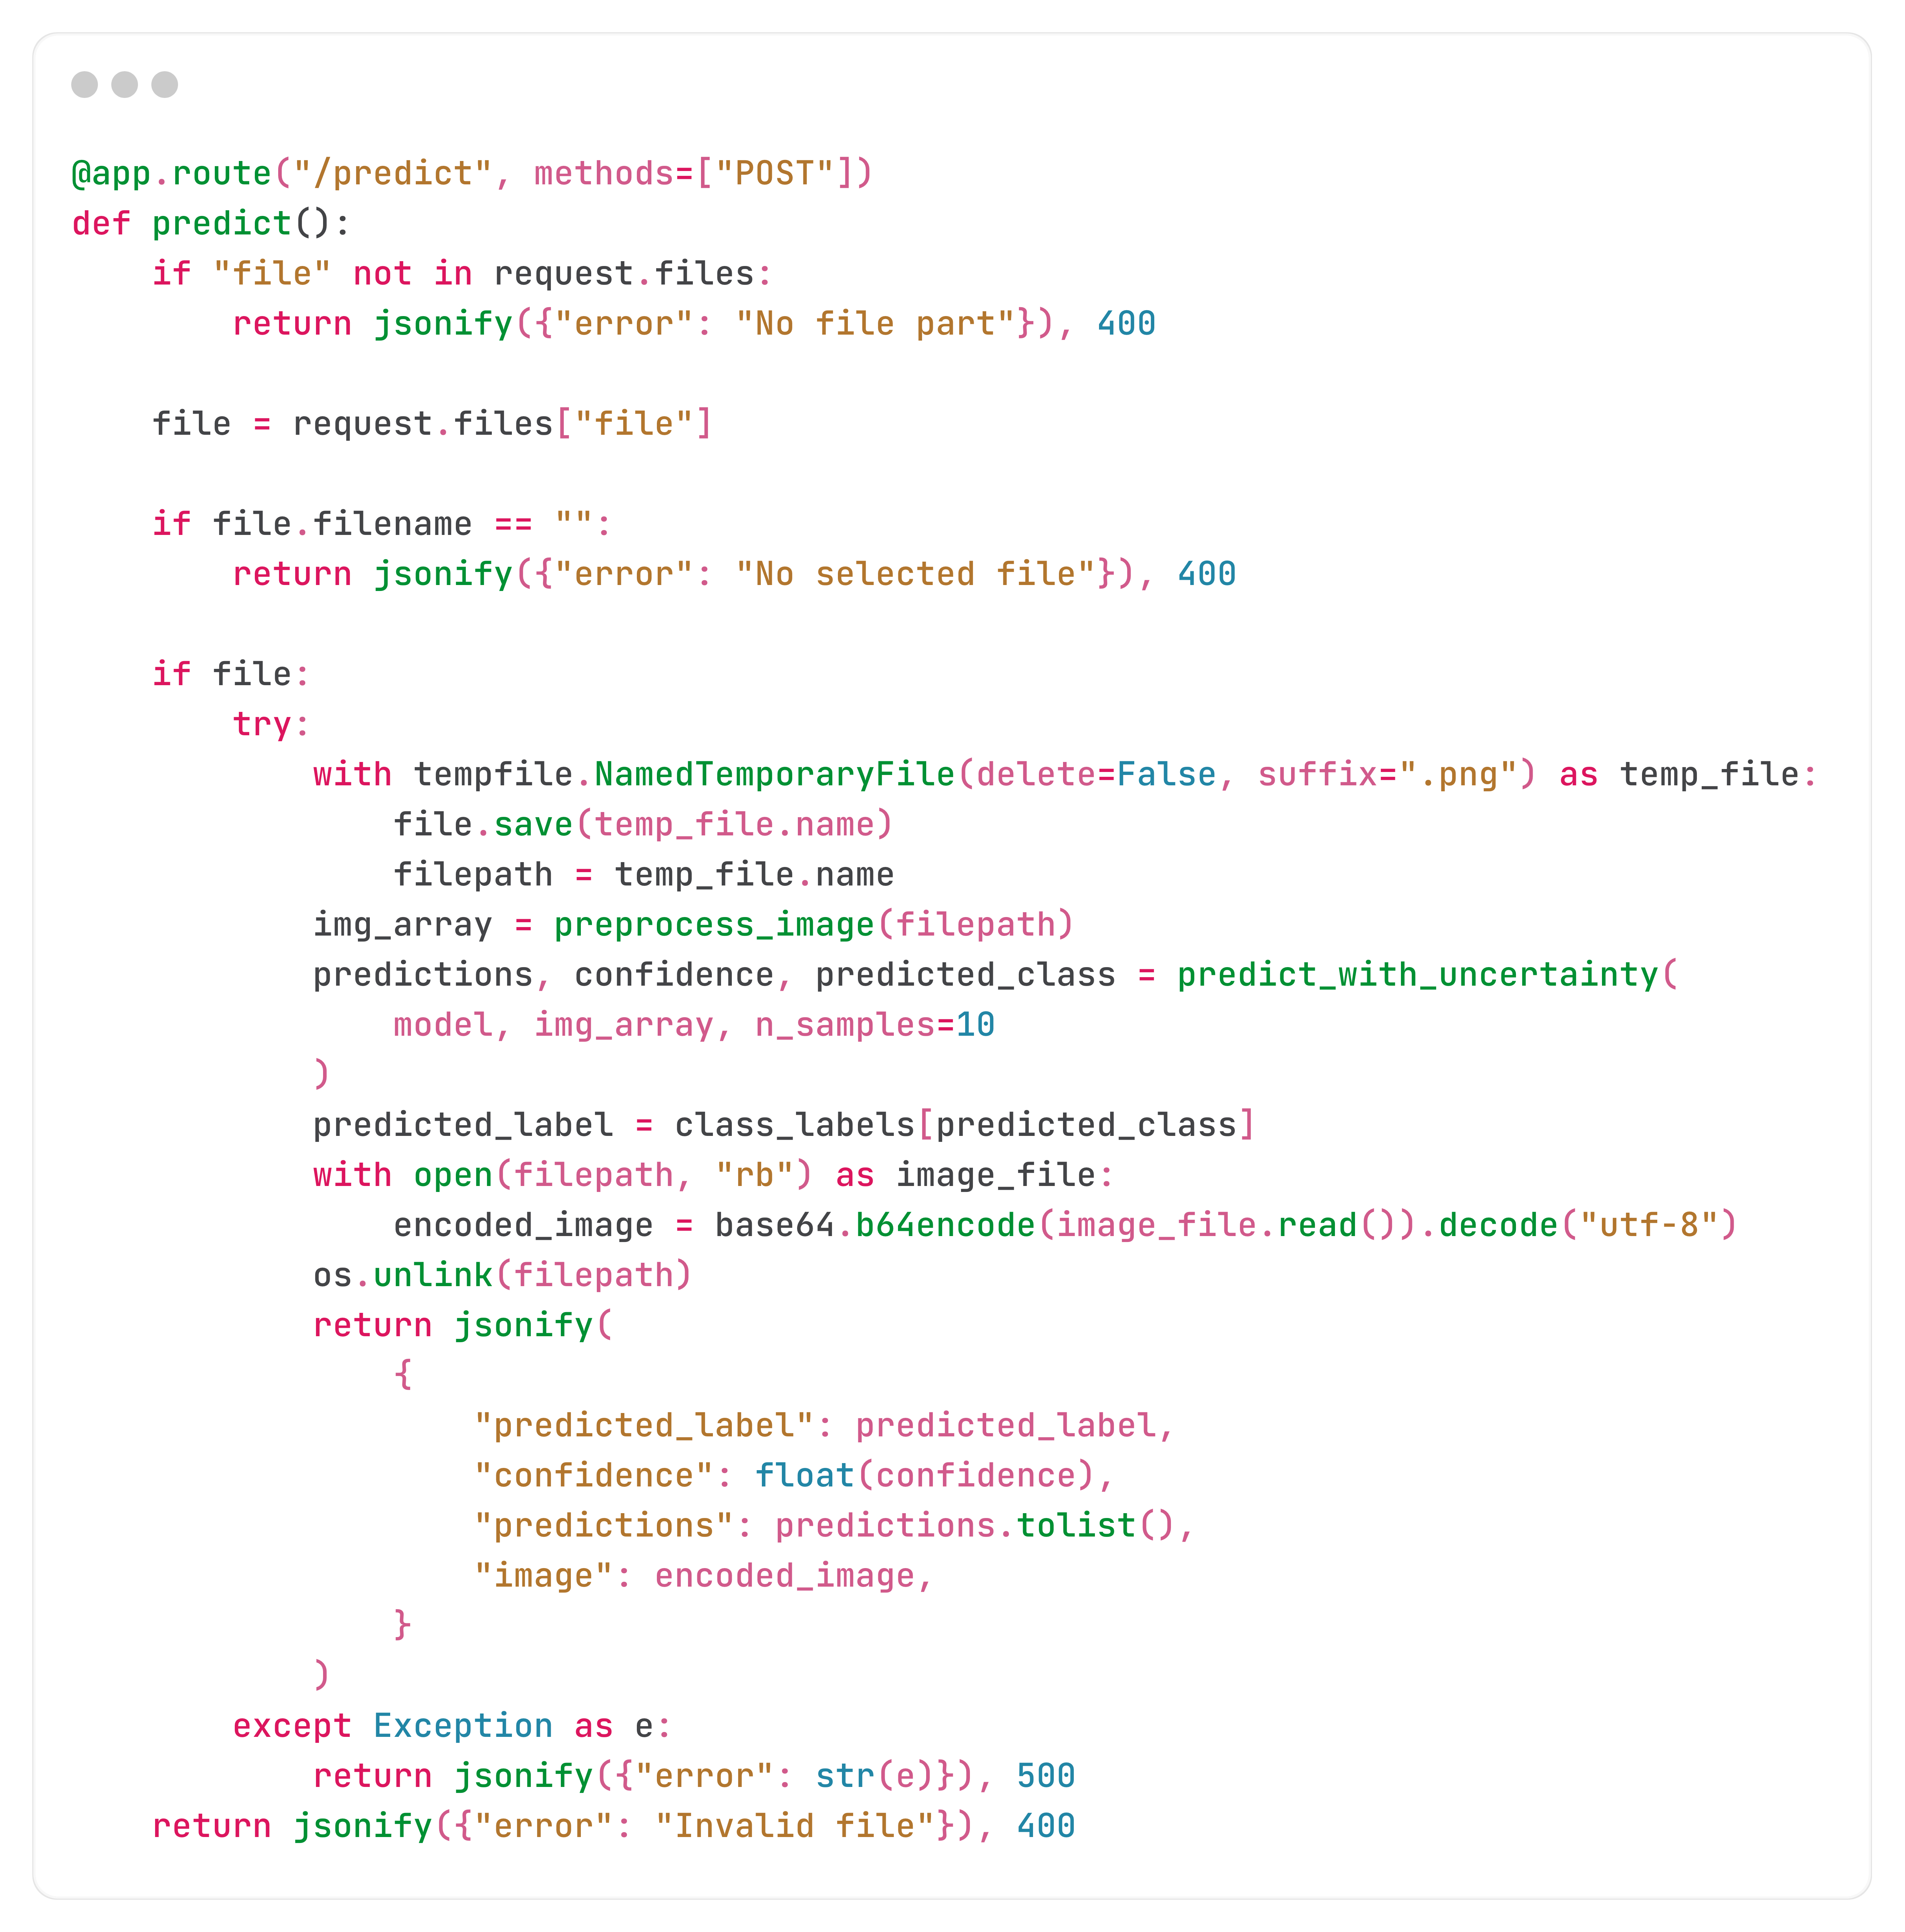
\includegraphics[width=0.8\columnwidth]{figures/imp_flask.png}  % Adjust the width to your liking
    \caption{code for flask api to predict the image} % Caption for the image
    \label{fig:imp_flask} % Label to reference the
\end{figure}
To connect the Front end with the back end prediction code we have made use to Flask API. It will be using RESTfull API. There is only one POST method that is used which will be sending the image, which once recieved in the backend will run the prediction model with uncertainity score and confidence score. The figure \ref{fig:imp_flask} shows you the code for predict method that is called to predict the image and also send you the confidence score. The confidence score and the predicted class will be then sent to the front end. The results will be then with a progresss bar.
\begin{enumerate} 
    \item Preprocesses the image to match the model's input requirements.
    \item Performs inference using the trained model.
    \item Computes uncertainty metrics using the Monte Carlo dropout technique.
    \item Returns the prediction results and uncertainty measures to the frontend.
\end{enumerate}


\chapter{Results and Discussion}
The results of the implementation of the code developed for creating a deep learning model for Alzheimer's disease using MRI image will be shows here in this section. The results consists of multi-class classification model’s performance metrics, an analysis of uncertainty estimations, performance analysis and a study of the insights gained from these. The results are analyzed in terms of overall accuracy of the model, class-wise performance of the model, and the advantages of incorporating uncertainty estimates to improve the model’s reliability and interpretability. To further underscore the benefits of the suggested approach, comparisons with base models are provided.

\section{Overall performance of the model}
The performance of the model was excellent. Once the model was created it was  run on the test dataset. It was able to predictes the four classes of Alzheimer's stages in our dataset exceptionally well. The model was consistent and reliability in correctly determining MRI images among the four target classes Mild Demented, Moderate Demented, Non-Demented, and Very Mild Demented were shown by its 99.55\% overall accuracy on the test dataset. Let's now compare that to the base model.
\begin{figure}[H]
    \centering
    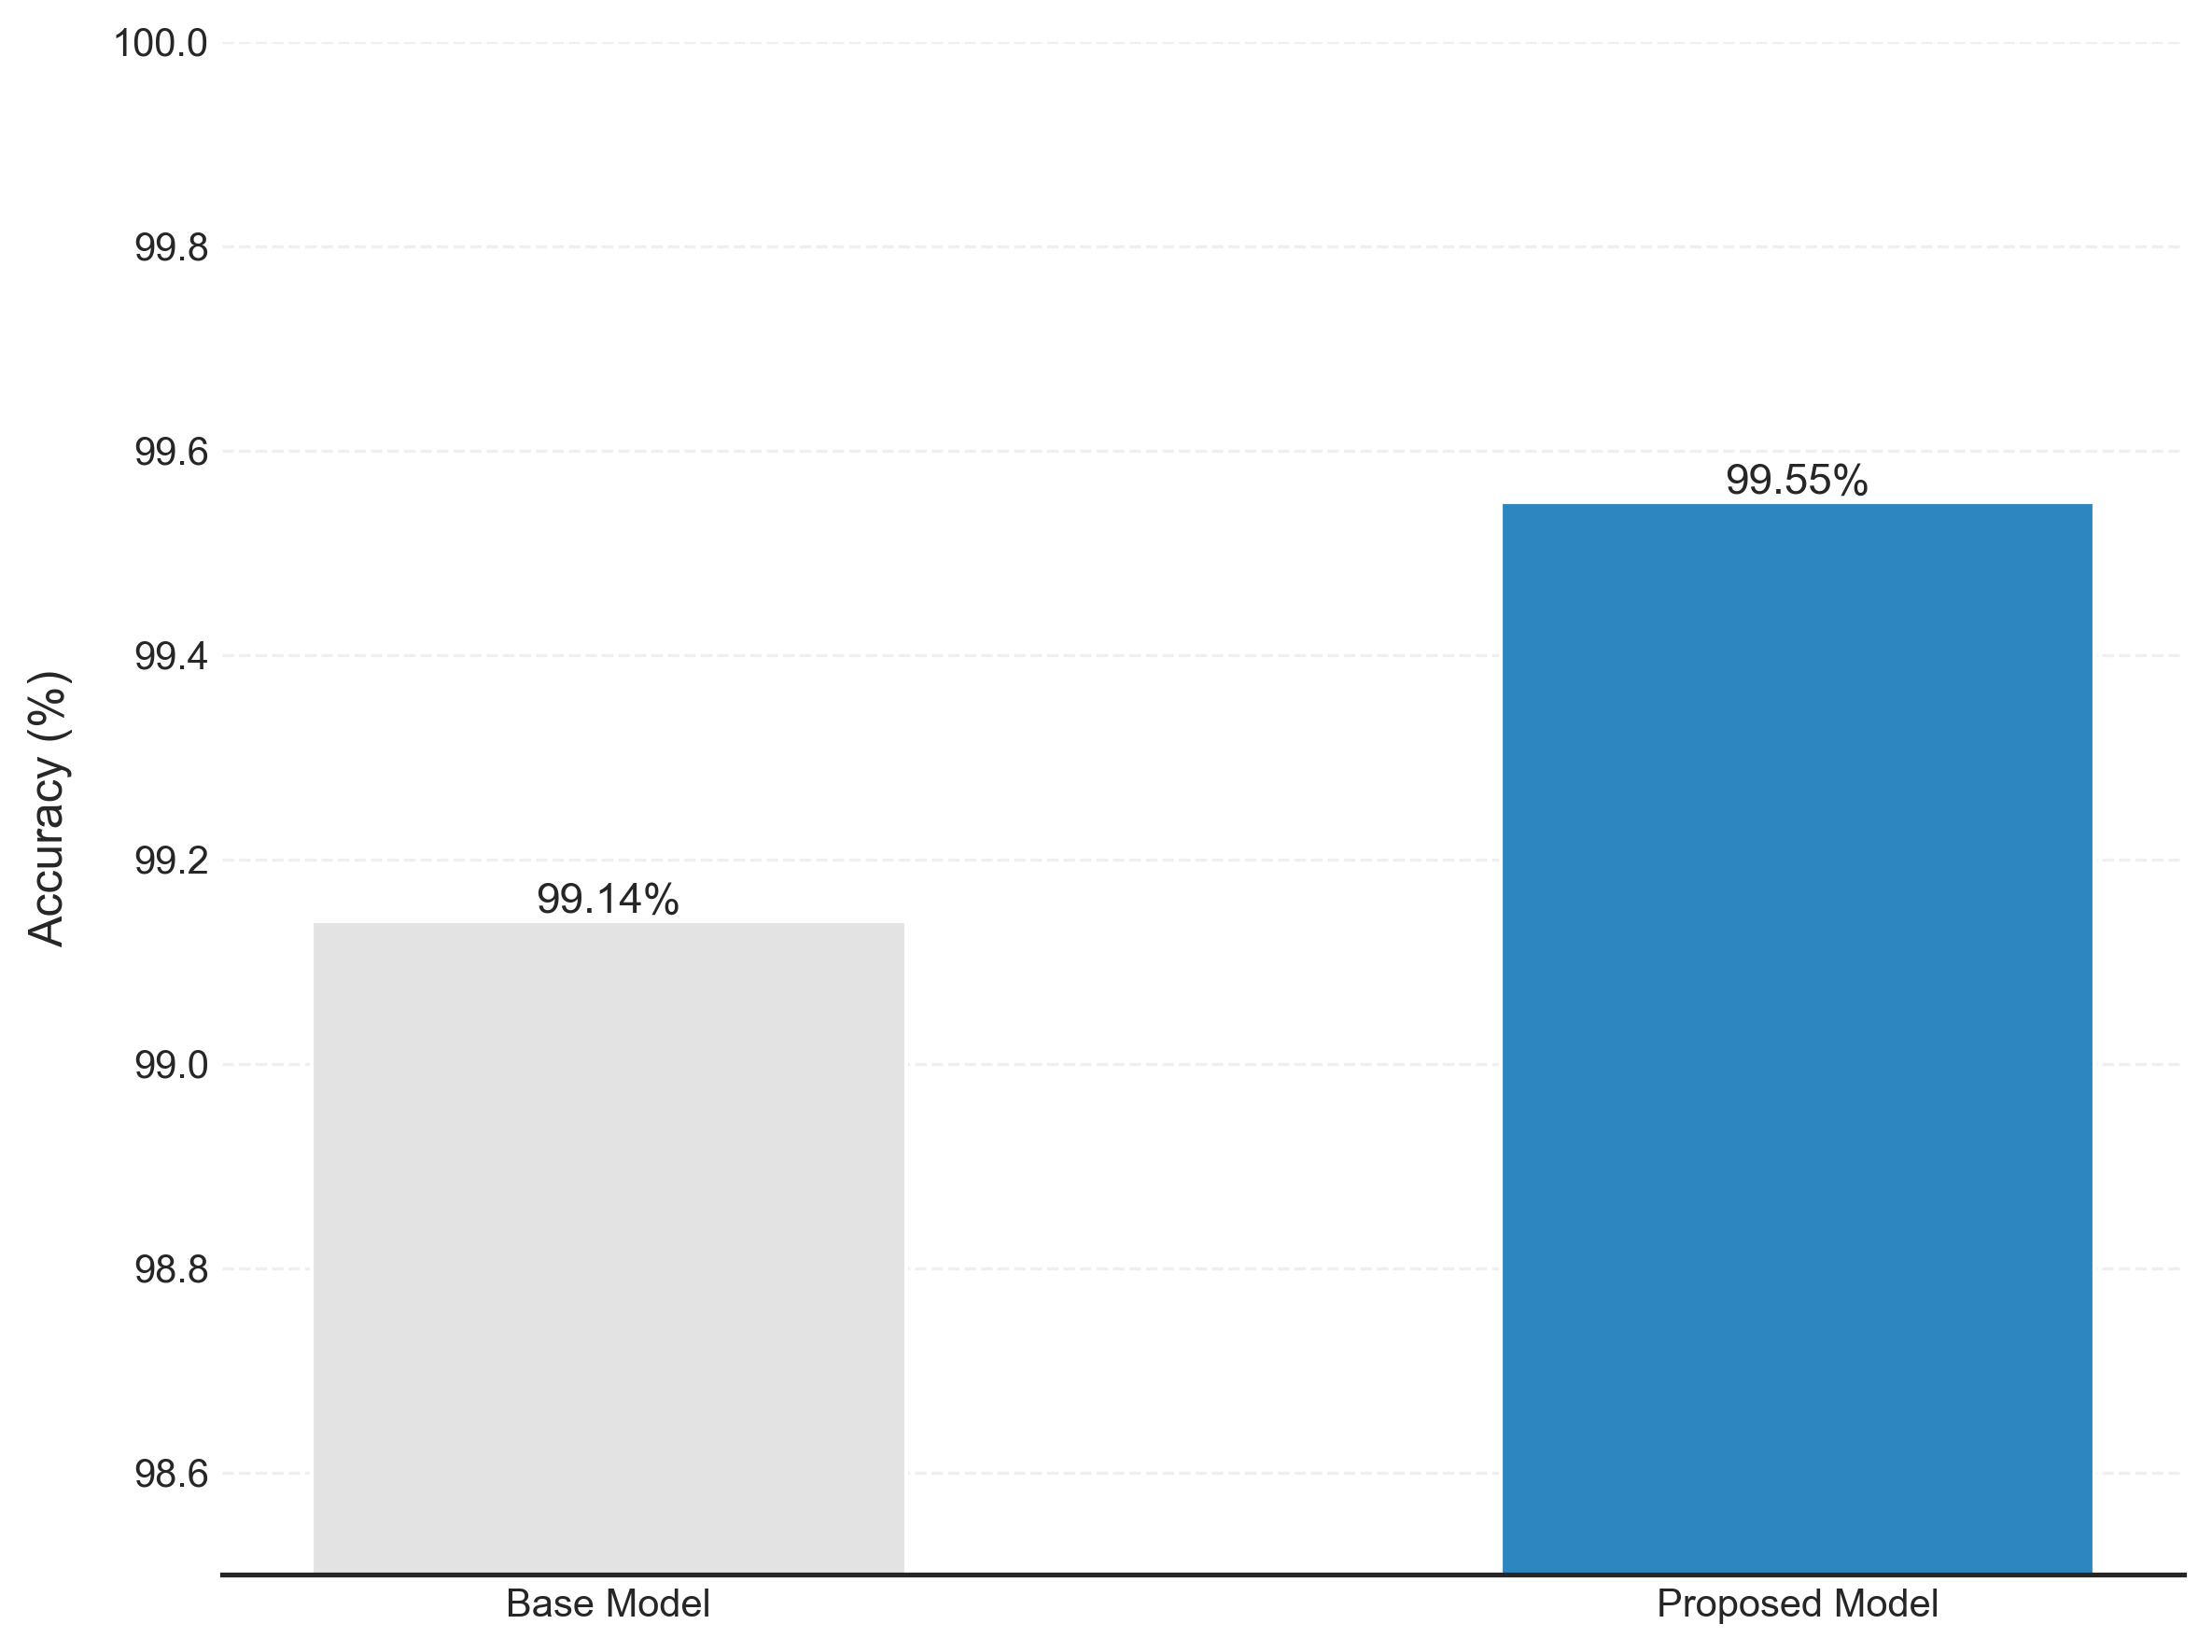
\includegraphics[width=0.6\columnwidth]{figures/res_model_comparison.png}  % Adjust the width to your liking
    \caption{figure showing the performance improvement in the proposed model (Higher the Better)} % Caption for the image
    \label{fig:res_model_comparison} % Label to reference the
\end{figure}
Note: the figure \ref{fig:res_model_comparison} is zoomed in between 99\% to 99.1\% to view the performance impovement in the proposed model. And these numbers are based on my tests conducted on these same exacpt system specifications.
This figure figure \ref{fig:res_model_comparison} shows the slight improvement in the models accuracy percentage. This improve might look not very significant, but when it comes to a medical world even a sligtest of mistakes can major impact on a persons life. Hence this a good performance gain achieved.

\section{Evaluating Classwise the model using the Metrics Chosen}
\begin{table*}[h!]
    \centering
    \begin{tabular}{|l|c|c|c|c|c|}
    \hline
    \textbf{Class} & \textbf{Precision} & \textbf{Recall} & \textbf{F1-Score} & \textbf{Accuracy} \\ \hline
    Mild Demented       & 0.99 & 1.00 & 1.00 & 1.00 \\ \hline
    Moderate Demented   & 1.00 & 1.00 & 1.00 & 1.00 \\ \hline
    Non Demented        & 0.99 & 0.99 & 0.99 & 0.99 \\ \hline
    Very Mild Demented  & 0.99 & 0.99 & 0.99 & 0.99 \\ \hline
    Macro Avg           & 0.99 & 0.99 & 0.99 & 0.99 \\ \hline
    Weighted Avg        & 0.99 & 0.99 & 0.99 & 0.99 \\ \hline
    \end{tabular}
    \caption{Table showing classwise evaluation metrics}
    \label{tab:class_eval}
\end{table*}
This class wise evaluation metrics in the figure \ref{tab:class_eval} provides a better idea of model's performance for each stages of the Alzheimers disease classes that are present in our dataset provided by the class-wise summary. In medical applications, where particular classes may need higher sensitivity because of their clinical implications, this precision is essential.For the Moderate Demented and Mild Demented classes, the model shows perfect scores that is Precision, Recall, F1-Score, and Accuracy, showing its great reliability in identifying these states. Strong generalization across all diagnostic classes is shown by the metrics for the Non-Demented and Very Mild Demented classes, which are a little lower but yet so close to ideal score that is 0.99 across all categories. So we can see that accross all the metrics the results are very balanced. Even the the dataset being moderately imbalanced did not have any effect on the final results as seen the weighted average row.


\section{visualizing the confidence score to the plot}
\begin{figure}[H]
    \centering
    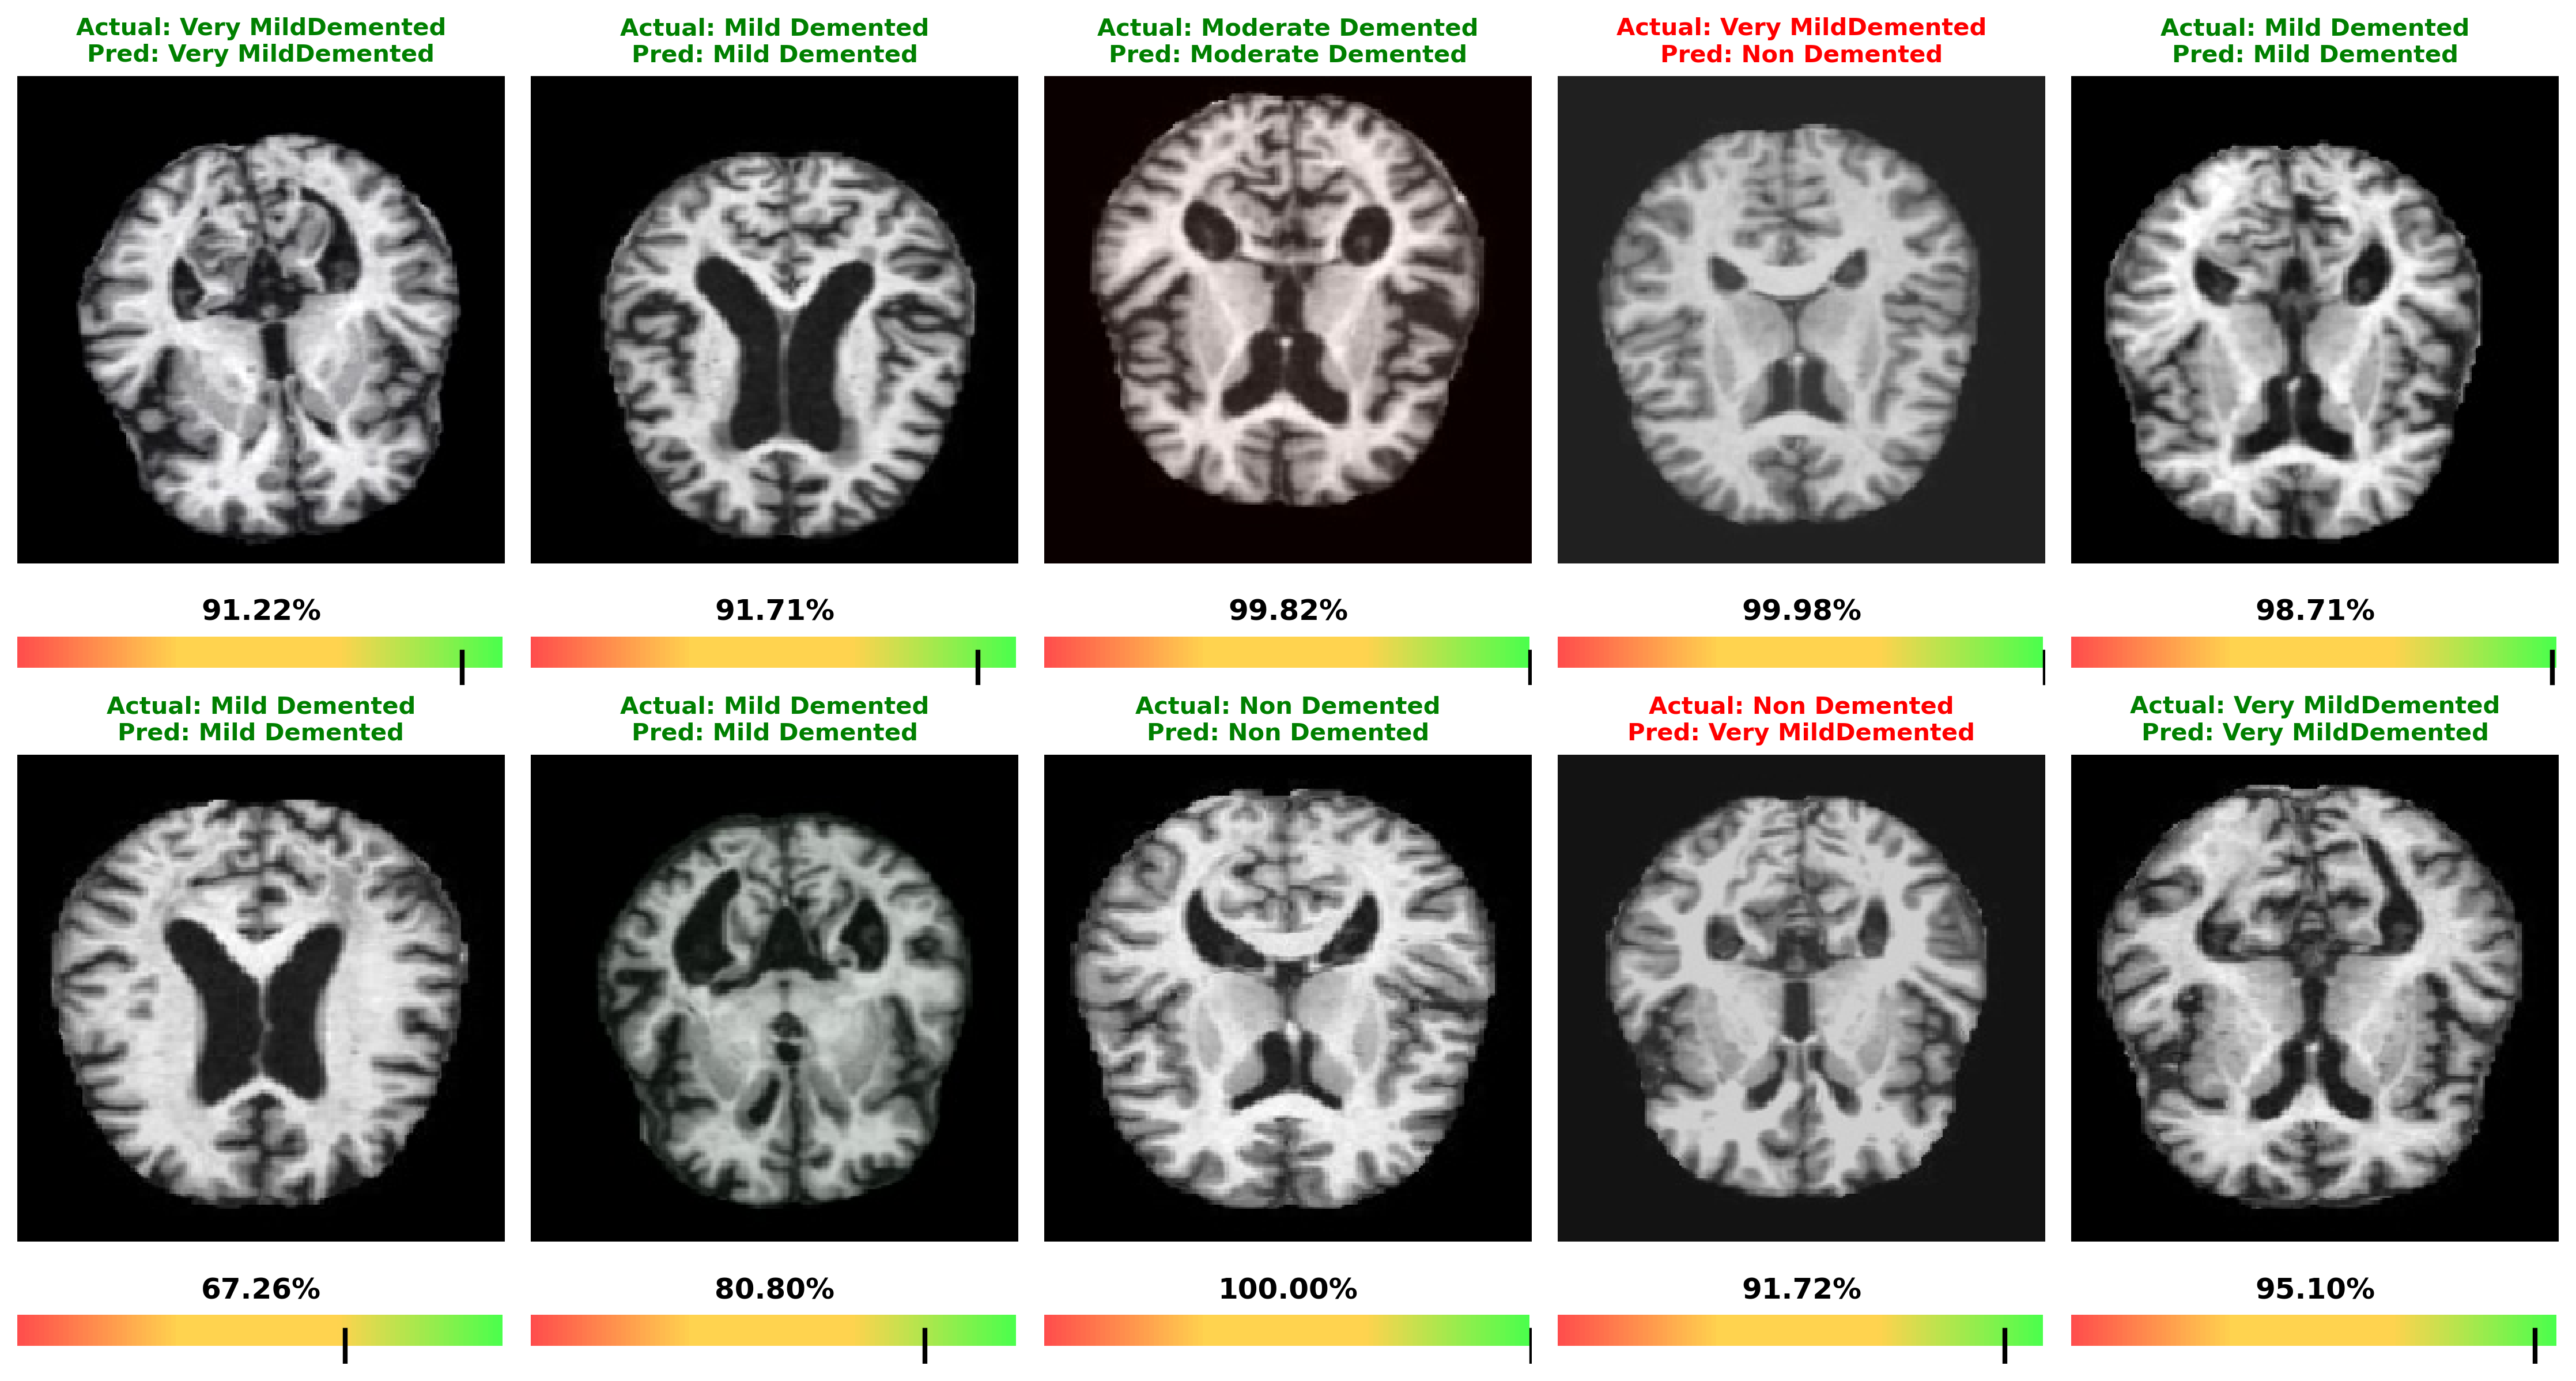
\includegraphics[width=0.8\columnwidth]{figures/res_uncertainity_sample_plot.png}  % Adjust the width to your liking
    \caption{image plotting the predicted class, actual class as well as the condifence percentage in progress bar.} % Caption for the image
    \label{fig:res_uncertainity_sample_plot} % Label to reference the
\end{figure}
A sample code was writen to predict a sample of 10 image and plot them in a image and show the confidence(1 - uncertainity) indicator  as a progress bar. The figure \ref{fig:res_uncertainity_sample_plot} show us as plot of these sample 10 images. As you can see in this figure out of the 10 images except the 2 images the rest of the images were predicted correctly. The images which are predicted wrong , the text is been highlighted in red. And this image is a proof why including confidence score is such a gamechanger. Because if you see the first image in the second row even though the image class is predicted correctly, the model does not look confident of this class. When there are scenarios where a models get's a input which is different from the one's it has been trained on it's tends to be uncertain. This is where having this as a output will make sure that the clinicians take further action and analysis thes MRI's further and take a informed decision.

\section{Model implementation on the WebPage}
\begin{figure}[H]
    \centering
    \subfloat[step 1: Upload and preview image]{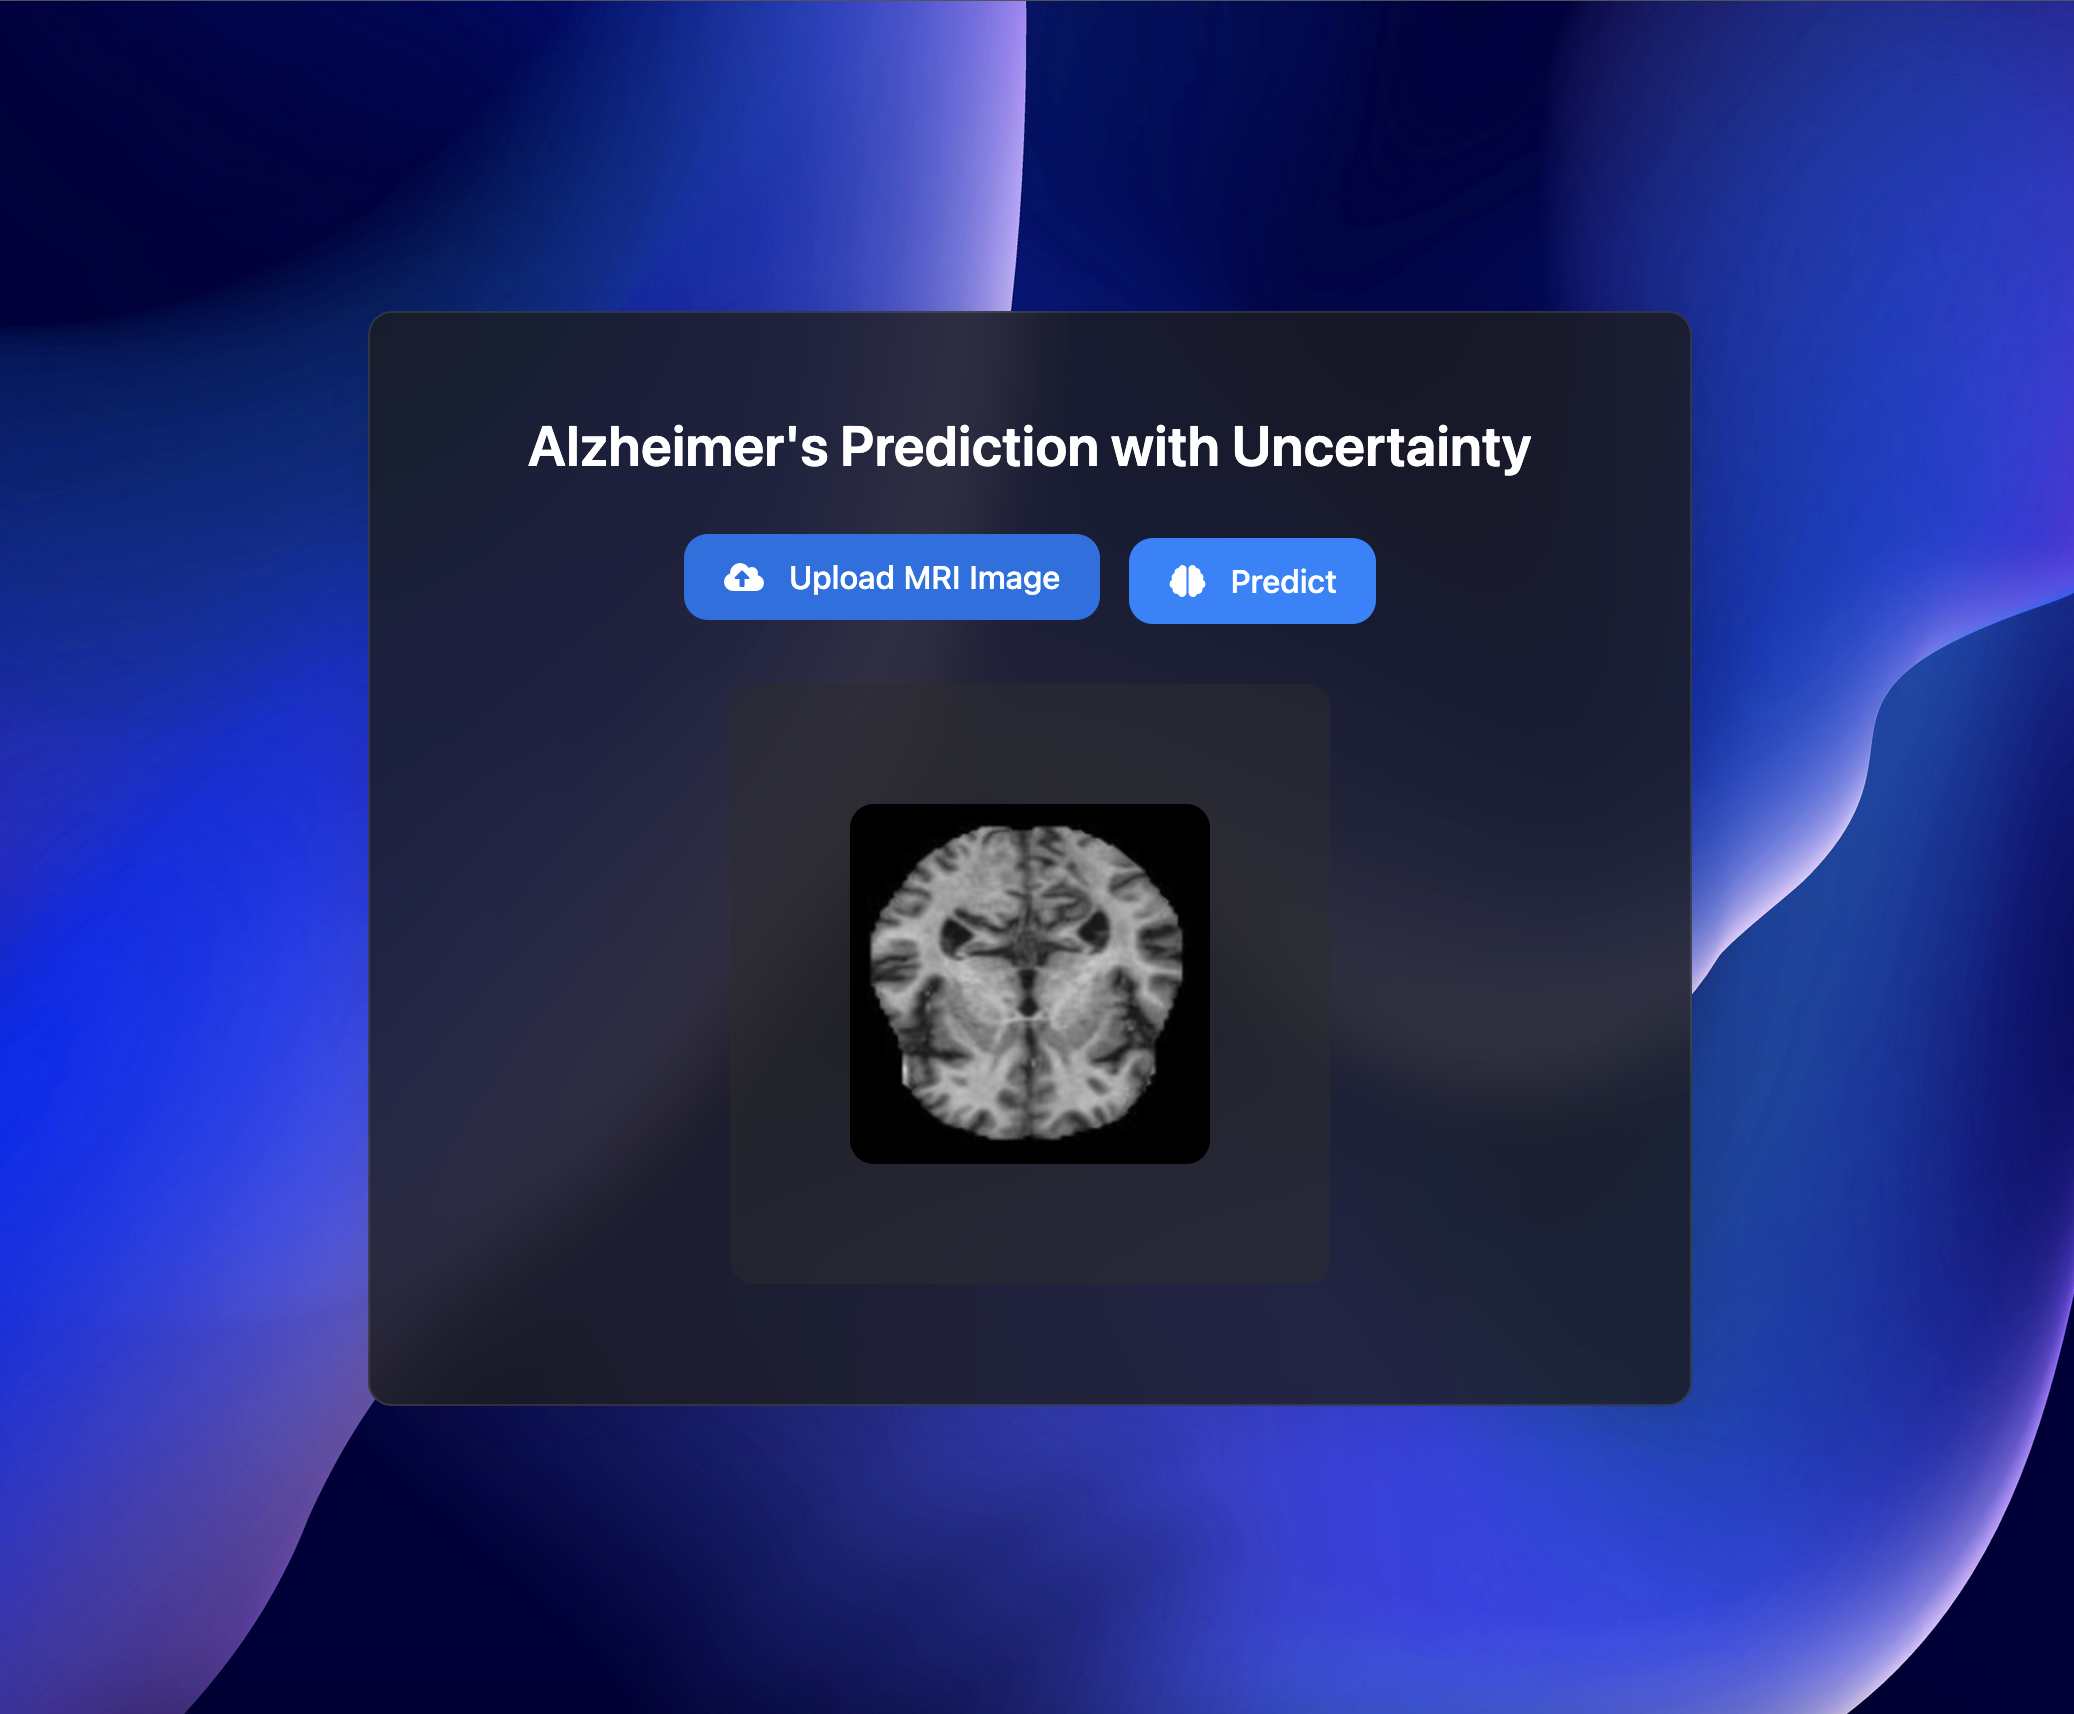
\includegraphics
    [width=0.45\textwidth]{figures/imp_webapp1.png}}
    \label{fig:webapp_subfig_a}
    \hfill
    \subfloat[step 2: Predict the image class with confidence score]
    {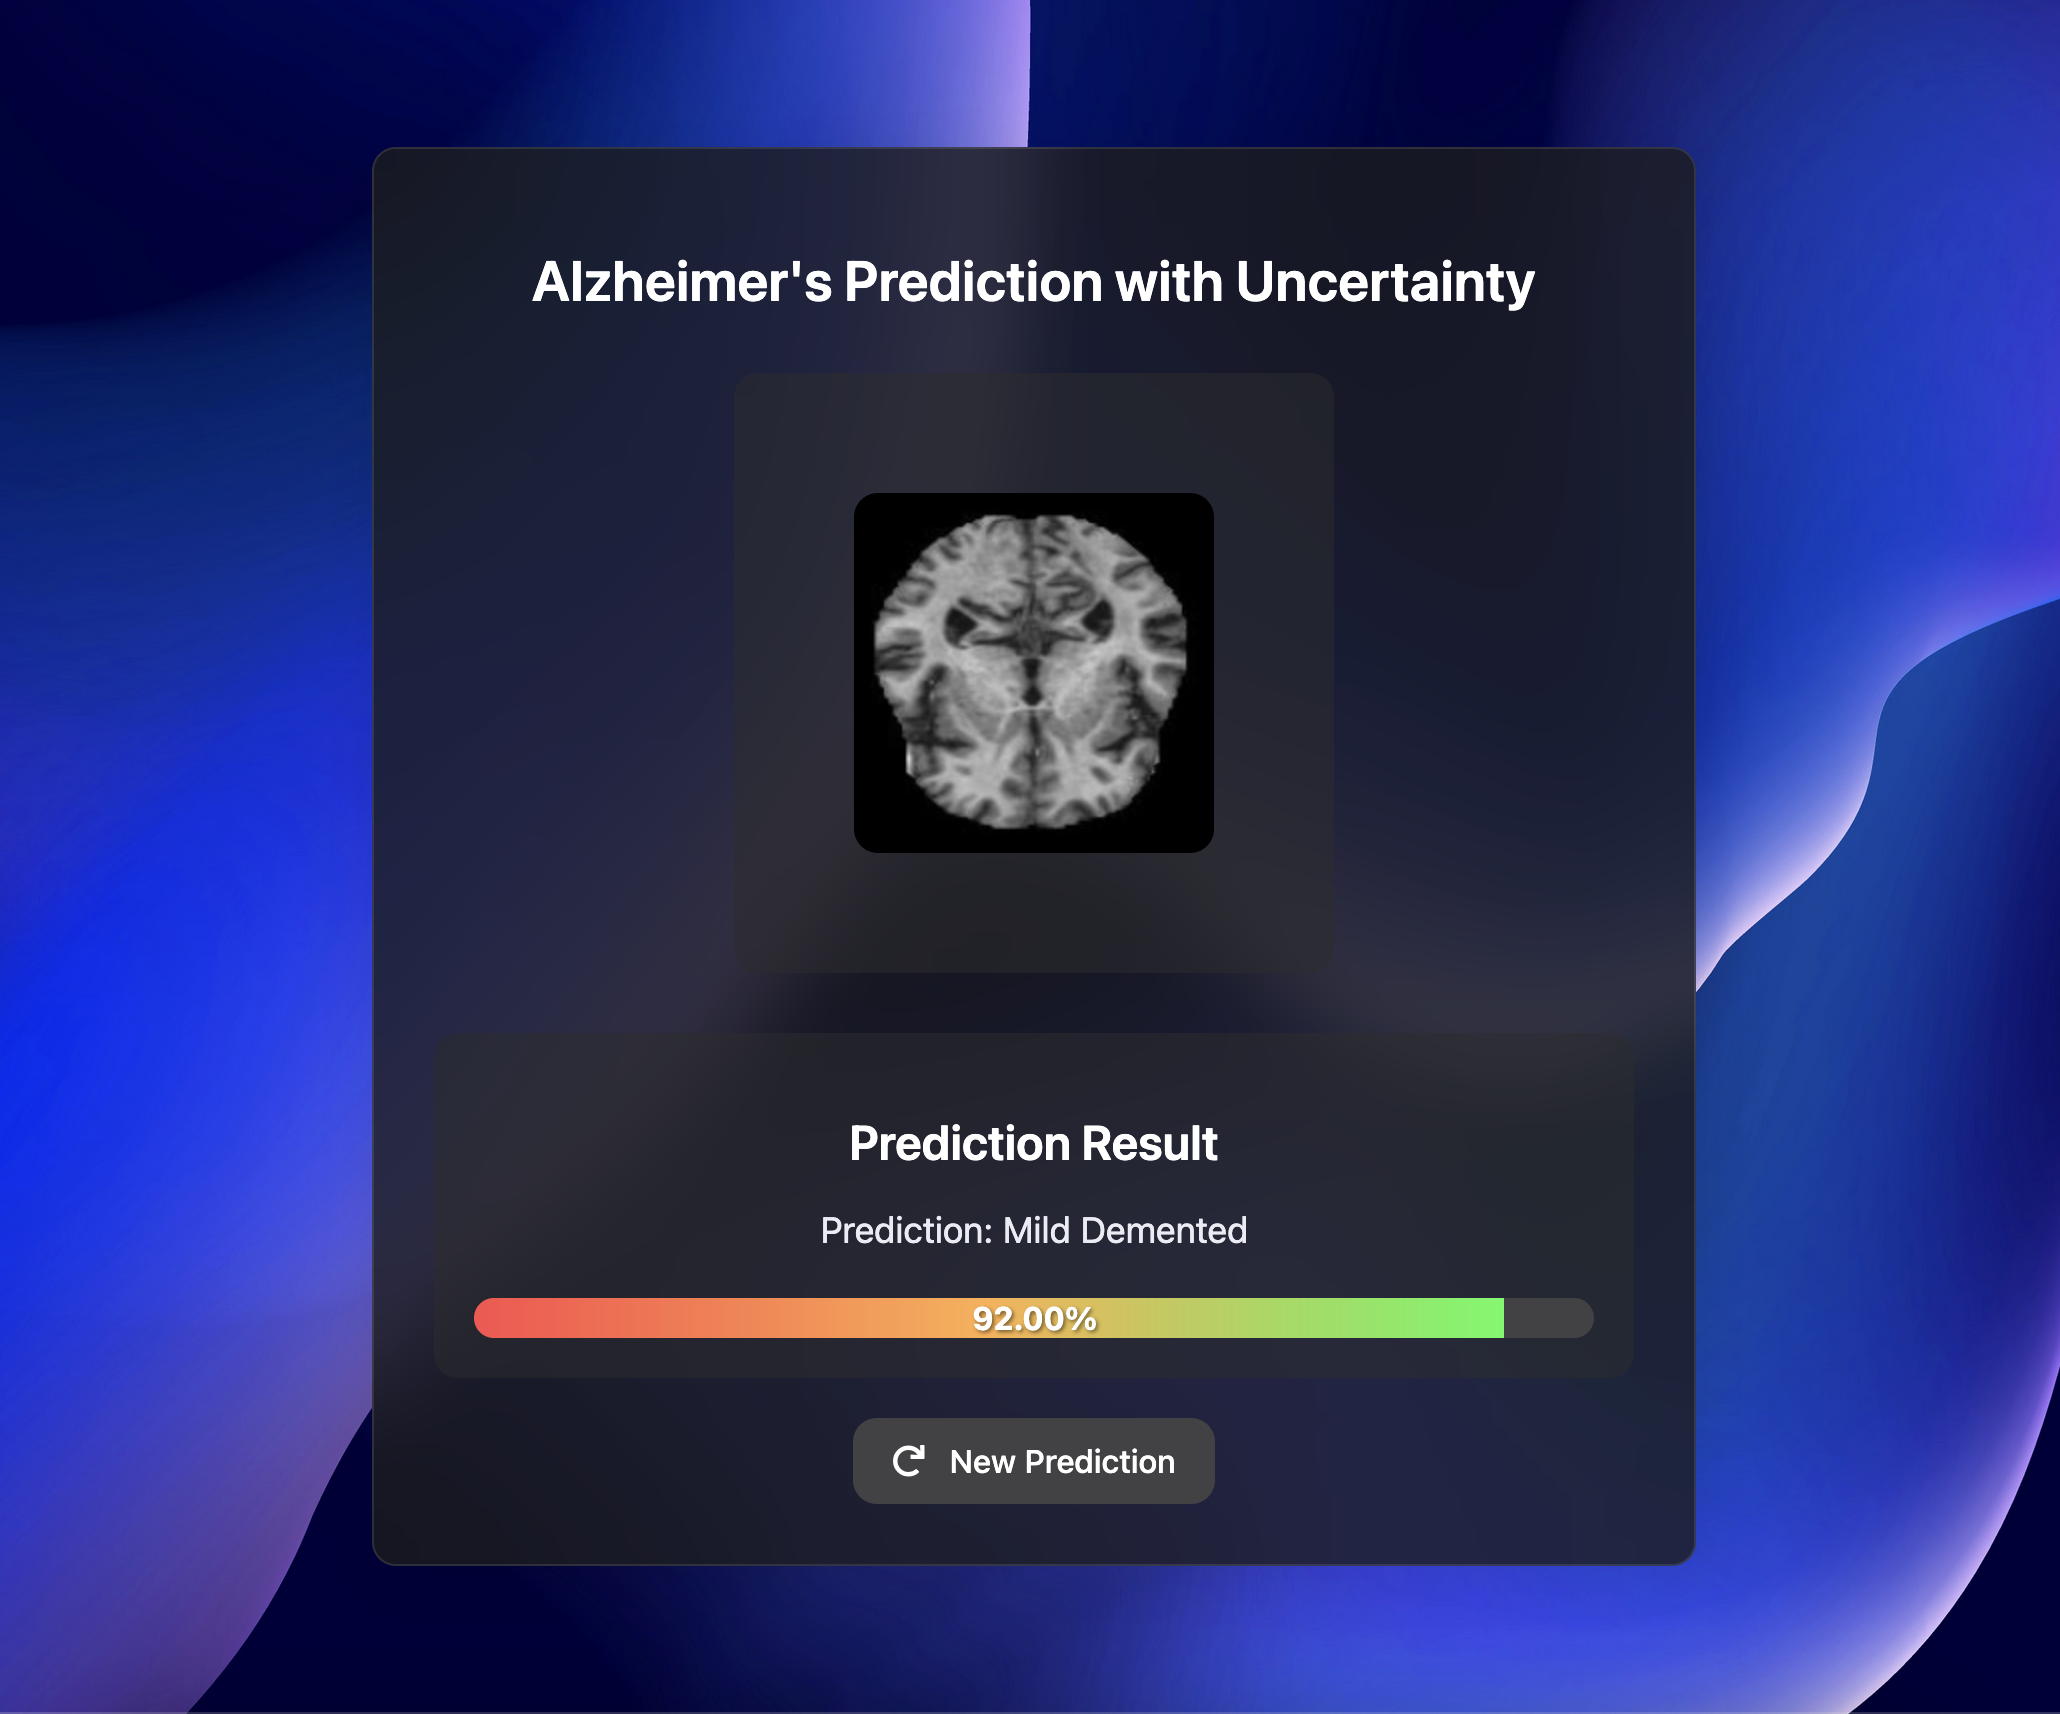
\includegraphics[width=0.45\textwidth]{figures/imp_webapp2.png}}
    \label{fig:webapp_subfig_b}
    \caption{Image Classification Web Application Workflow}
    \label{fig:webapp_workflow}
\end{figure}
The figure \ref{fig:webapp_workflow} shows the final images of a simple webpage application where in the initial screen there are two buttons. Upload and predict. The user needs to click on the upload button first which will take him to the image selection dialogue box. Once selected it will give a preview of the image. Next, predict botton needs to be clicked. Which make a predict API call. The model is  connected to the webpage using Flask architecture. Using RESTfull API's a method called 'predict' is created. The API will then send the predicted class and the confidence score in return. The final screen has progress bar which has a gradient of red to green. That is where the uncertainity score is shown to the user. Anything below 80\% is considered as bad confidence score. If in that case further study needs needs to be done on that case. 

\section{Model Training performance and Comparision with base model}
\begin{table}[h!]
    \centering
    \caption{Computing time comparison between the base model and the proposed model (in seconds).}
    \label{tab:timing-results}
    \begin{tabular}{|l|c|c|}
        \hline
        \textbf{Stage} & \textbf{Base Model} & \textbf{Proposed Model} \\
        \hline
        Data Loading and Preprocessing & 0.01 & 0.00 \\
        Model Building & 0.51 & 0.56 \\
        Model Training & 1041.34 & 242.27 \\
        Model Evaluation & 12.22 & 3.34 \\
        Prediction & 0.00 & 67.59 \\
        \hline
    \end{tabular}
\end{table}

\begin{figure}[h!]
    \centering
    % Row 1: Two plots side by side
    \subfloat[\tiny\itshape Data Loading and Preprocessing\label{fig:res_time_loading}]{
        \fbox{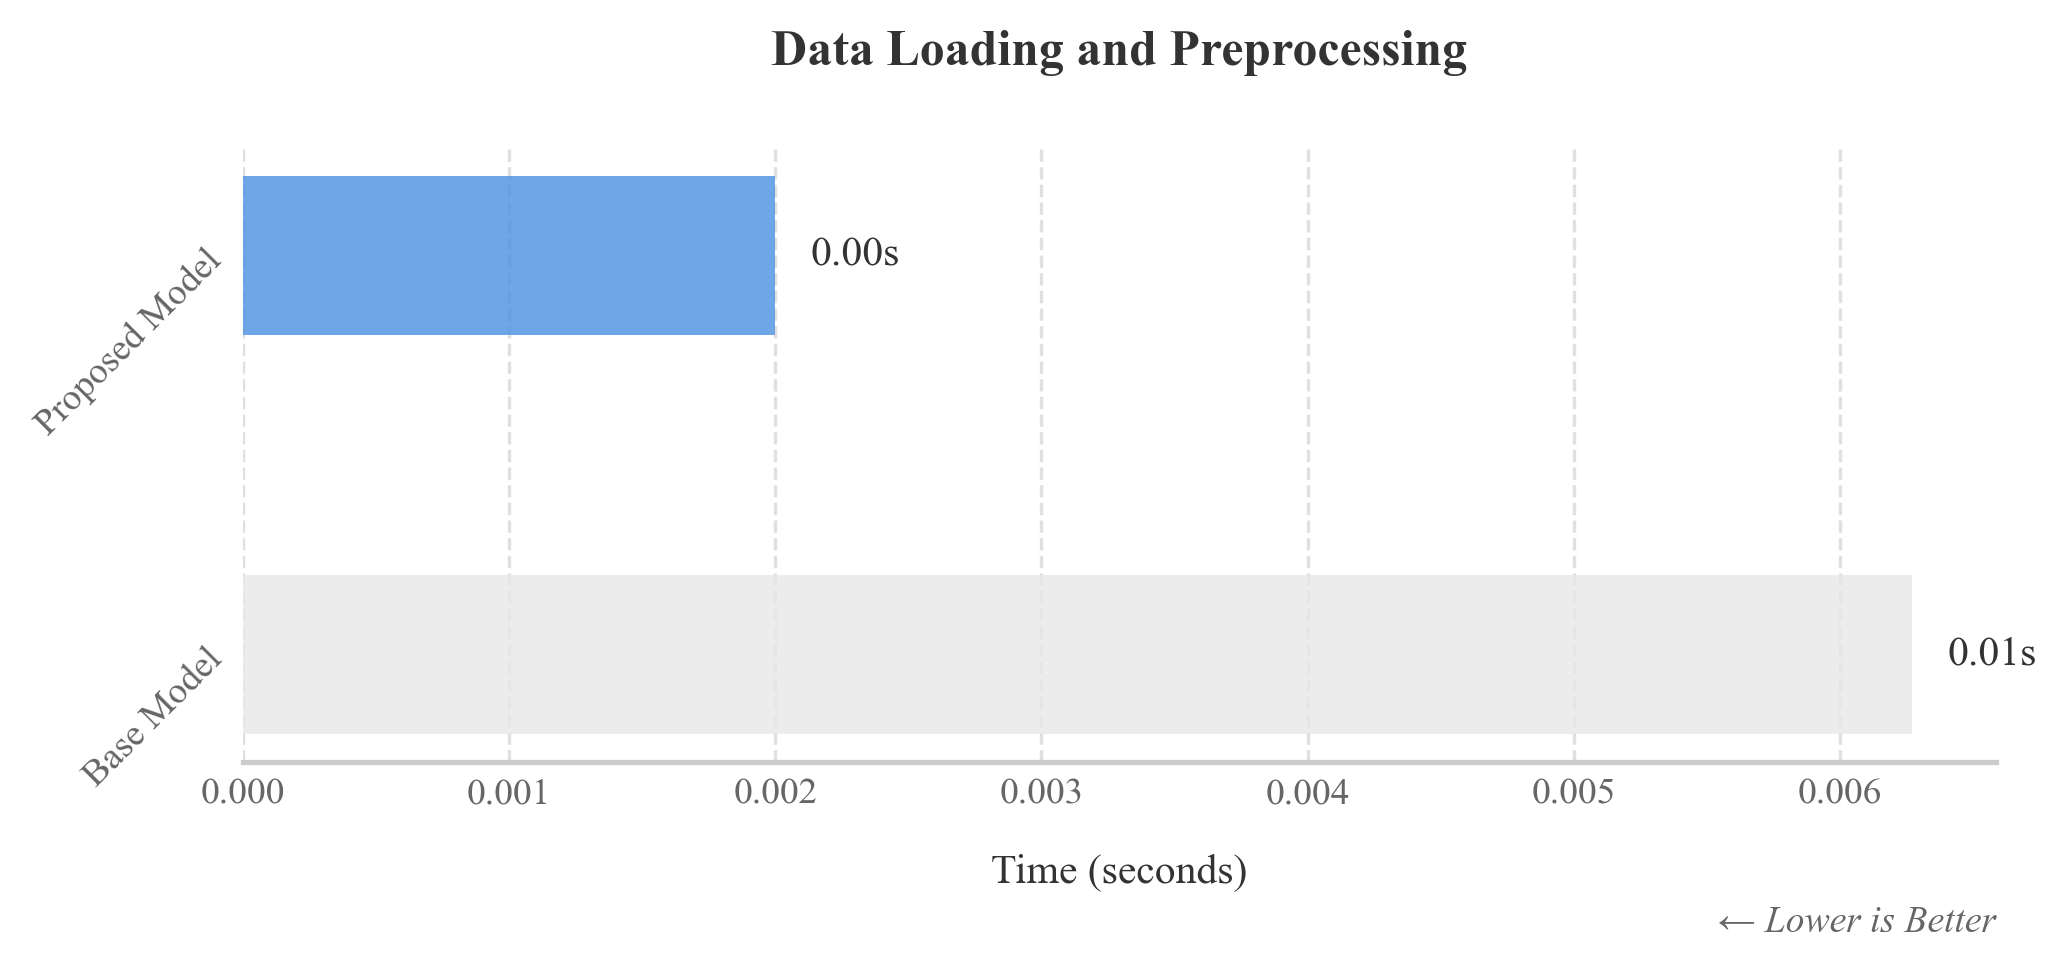
\includegraphics[width=0.45\textwidth]{figures/res_time_loading.png}}
    }
    \hfill
    \subfloat[\tiny\itshape Model Building\label{fig:res_time_building}]{
        \fbox{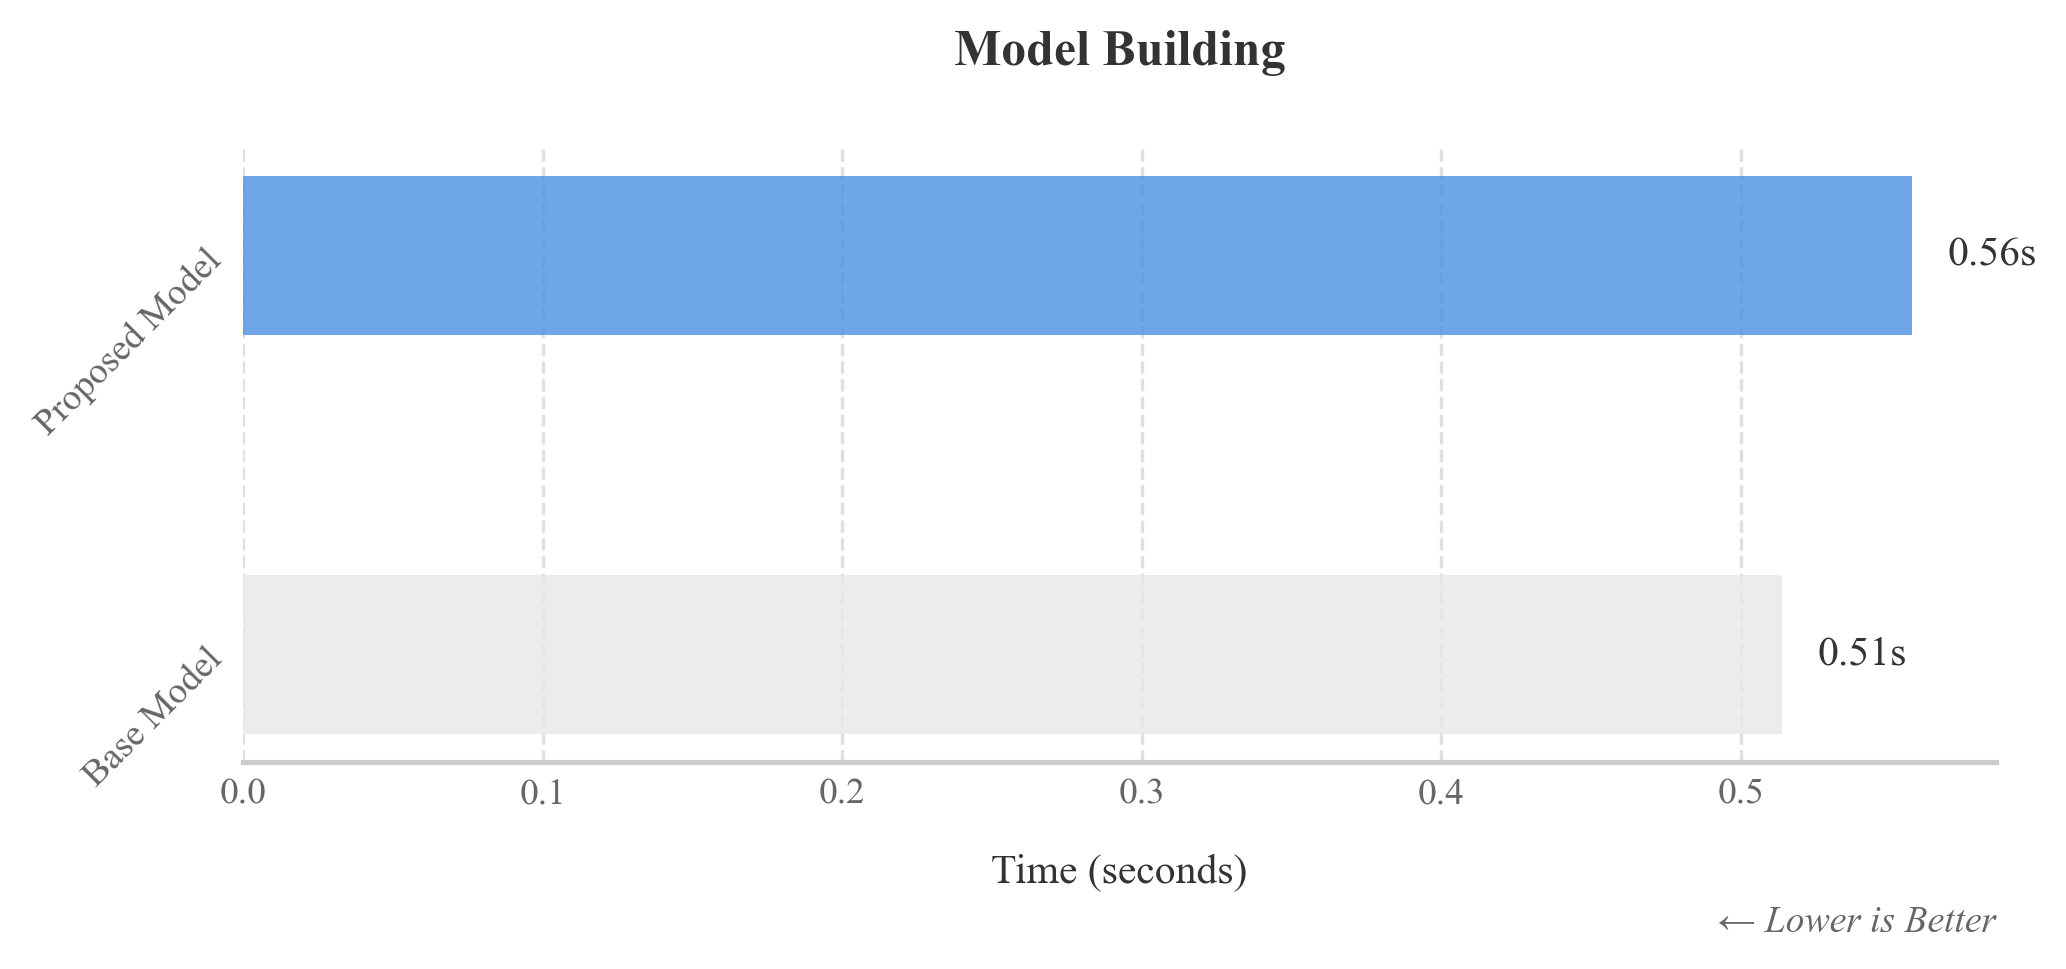
\includegraphics[width=0.45\textwidth]{figures/res_time_building.png}}
    }

    % Row 2: Two plots side by side
    \subfloat[\tiny\itshape Model Training\label{fig:res_time_training}]{
        \fbox{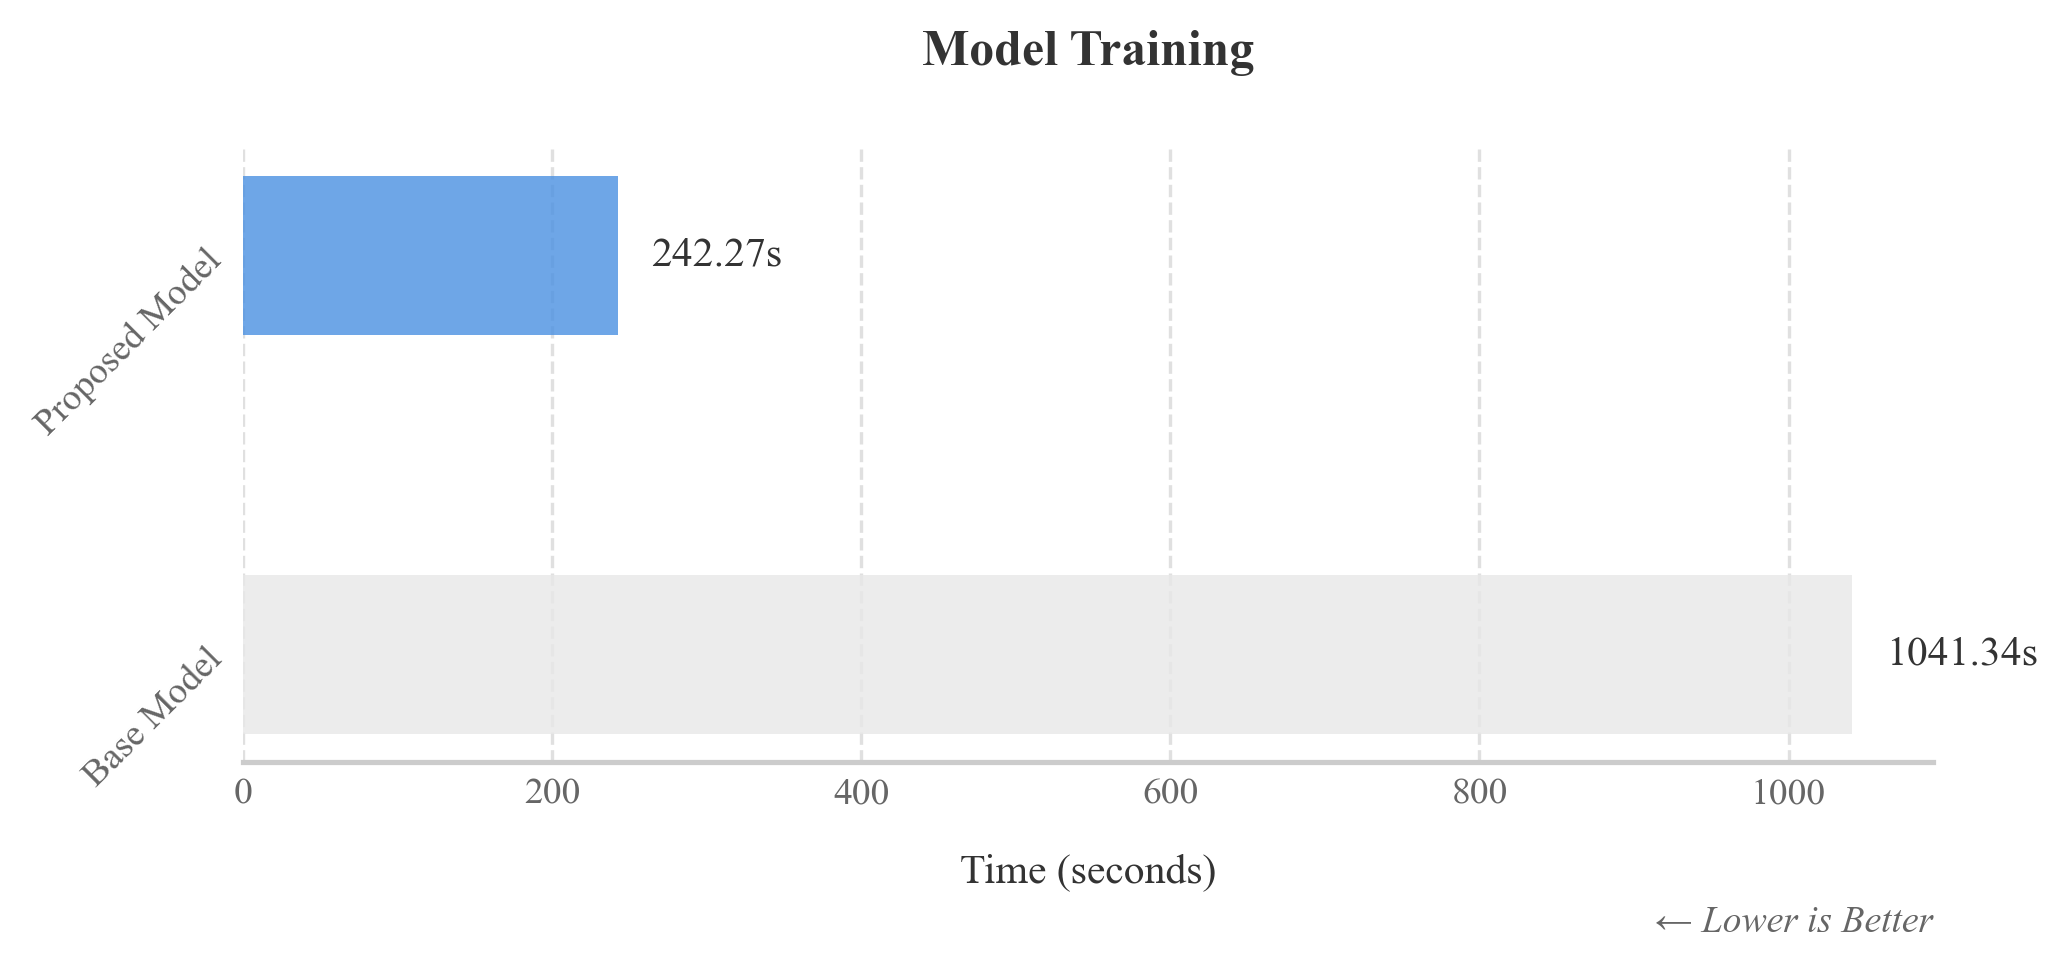
\includegraphics[width=0.45\textwidth]{figures/res_time_training.png}}
    }
    \hfill
    \subfloat[\tiny\itshape Model Evaluation\label{fig:res_time_evaluation}]{
        \fbox{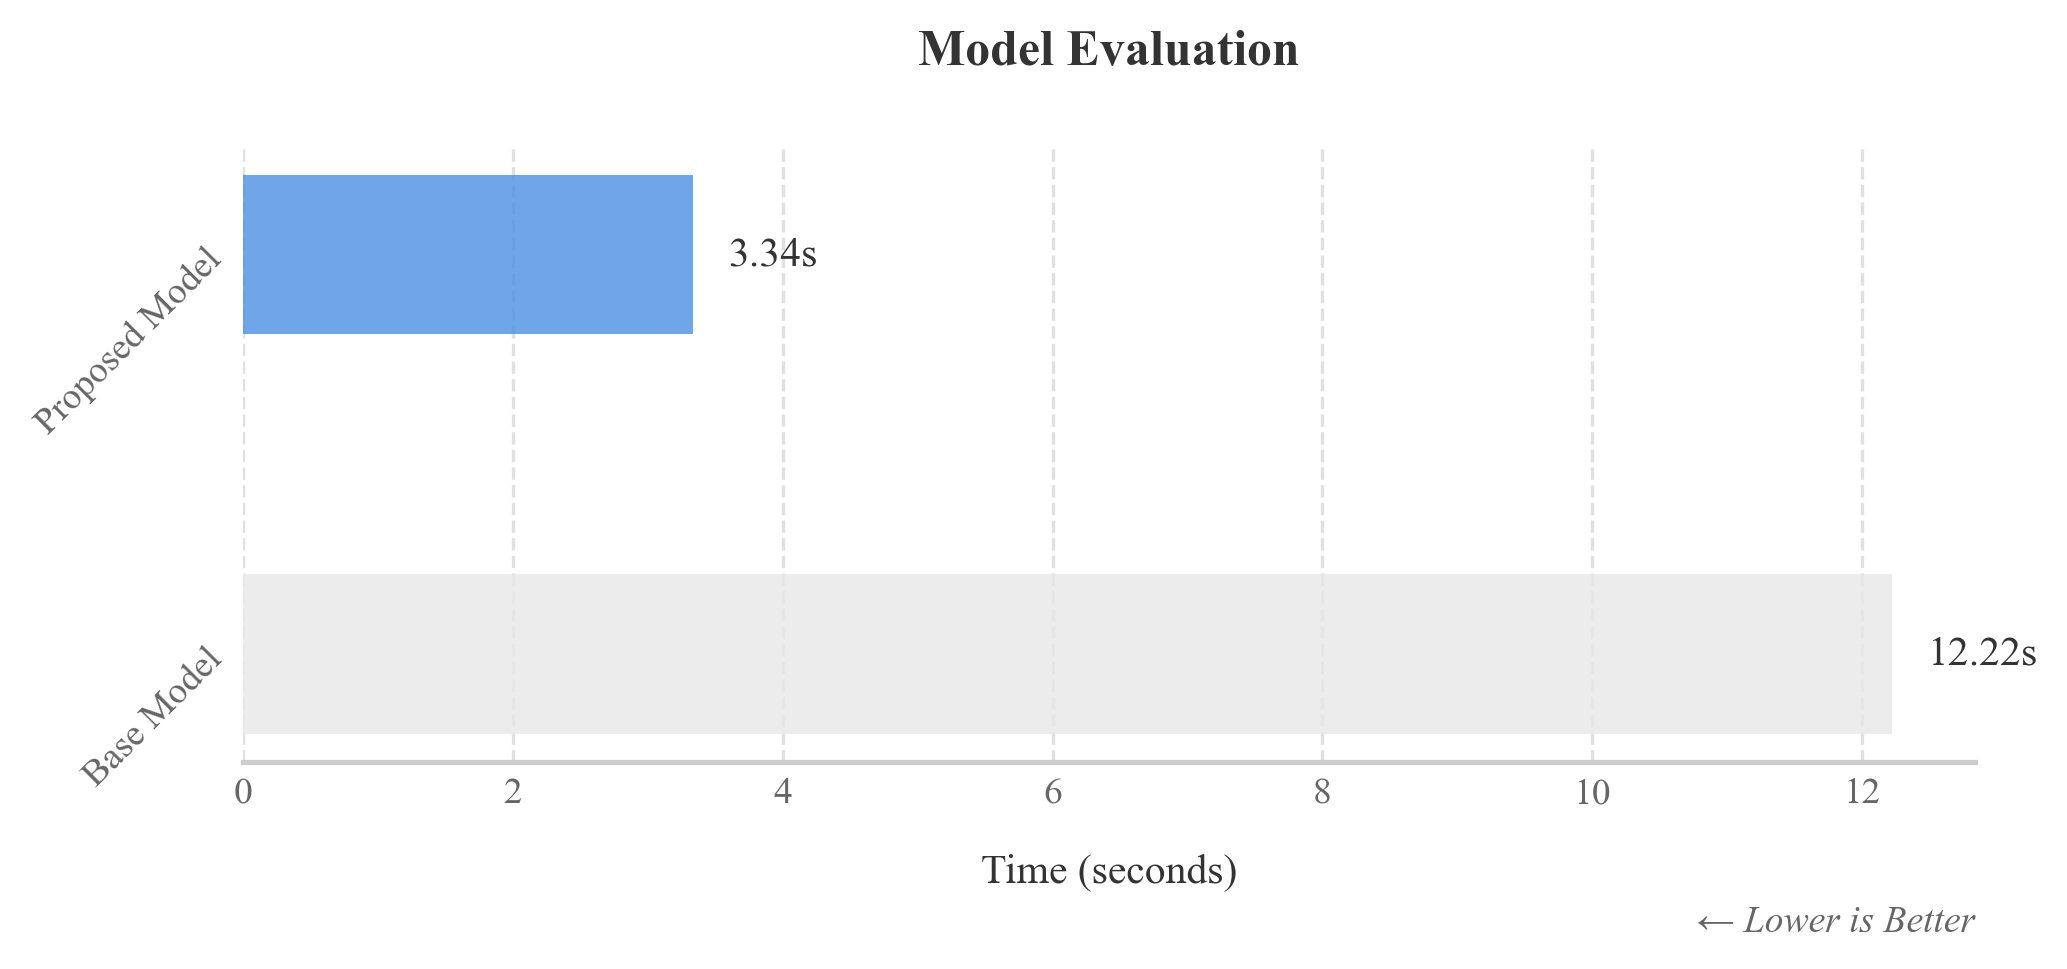
\includegraphics[width=0.45\textwidth]{figures/res_time_evaluation.png}}
    }

    % Row 3: Single centered plot
    \subfloat[\tiny\itshape Prediction Time\label{fig:res_time_prediction}]{
        \fbox{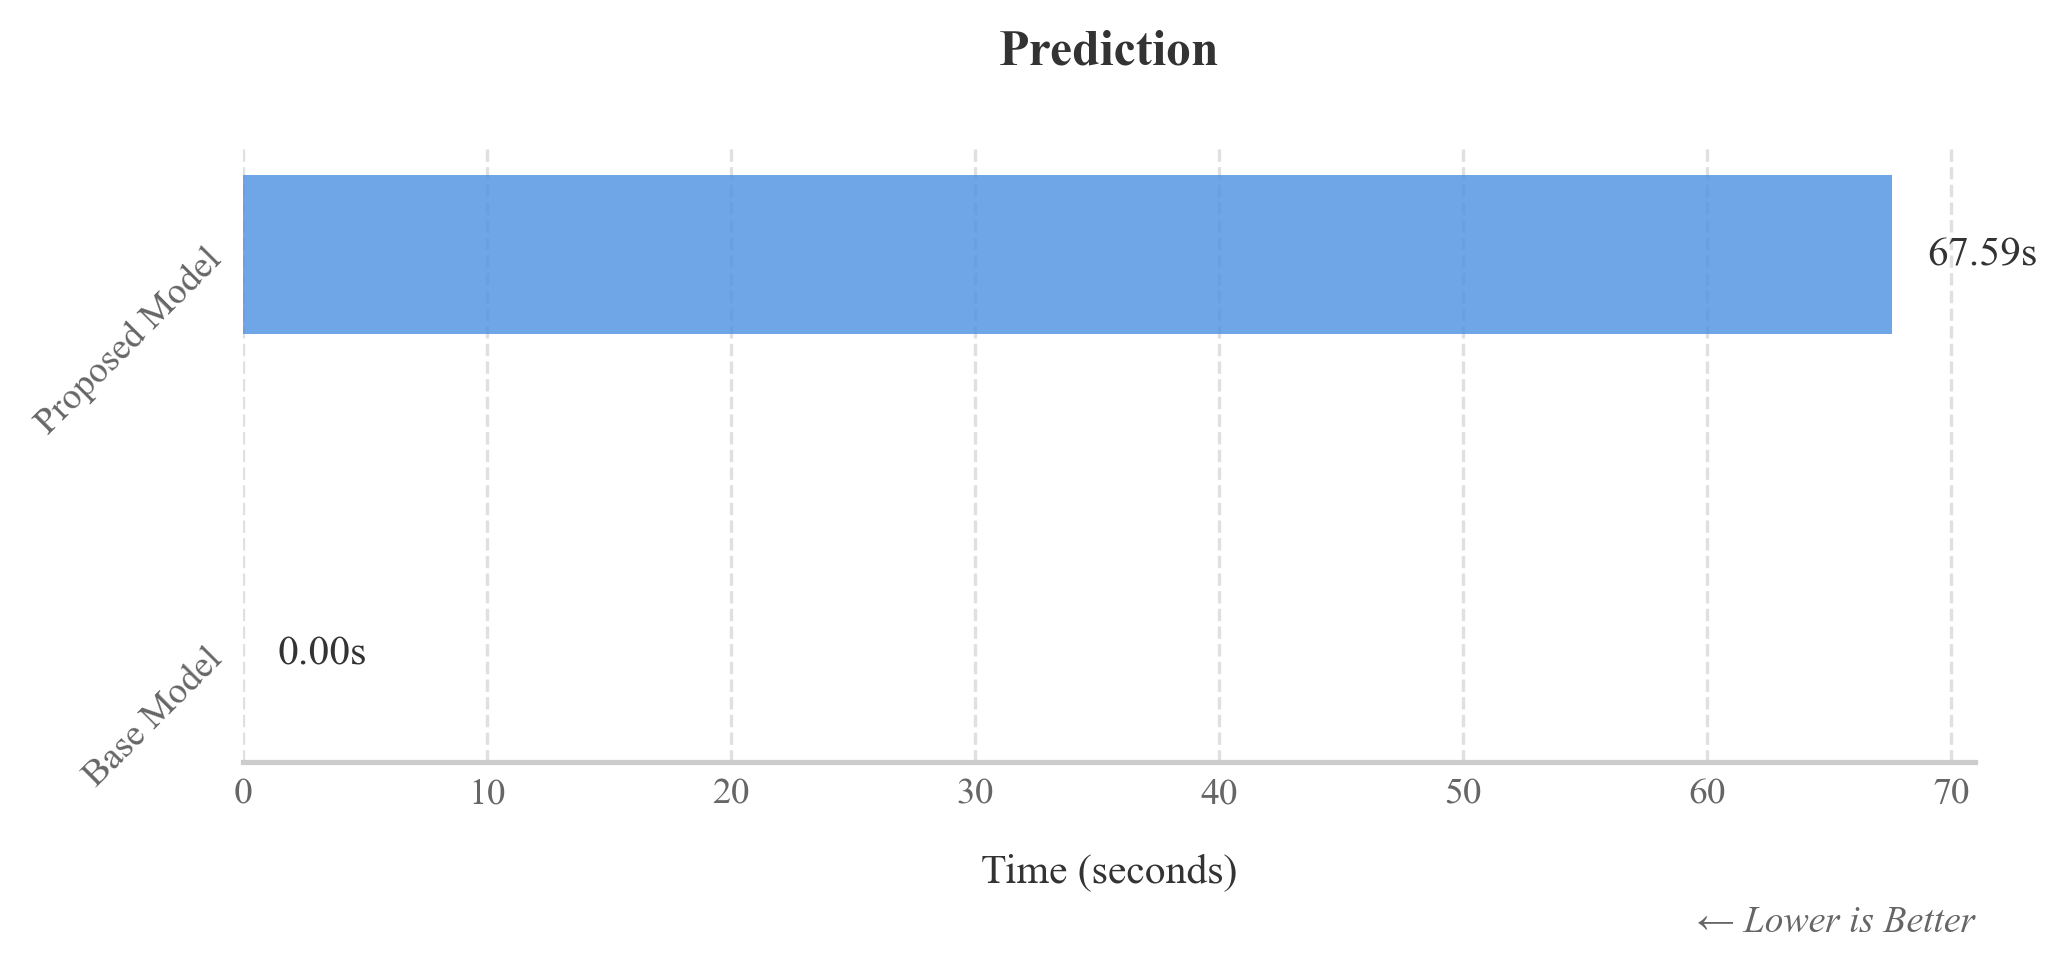
\includegraphics[width=0.55\textwidth]{figures/res_time_prediction.png}}
    }

    \caption{Computing time comparison between the base model and the proposed model for different stages of the pipeline. Lower values indicate better performance.}
    \label{fig:timing-comparisons}
\end{figure}

\subsection{Data Loading and Preprocessing}
The proposed model demonstrated a marginally faster time of 0.00 seconds compared to the base model of 0.01 seconds. This is very negligible and can be ignored due to the fact that 0.01 secs does not effect the computational cost. You can see this in the Figure~\ref{fig:res_time_loading}.

\subsection{Model Building}
While comes to Model building there 4 secs more taken by the proposed mode. This maybe due to the fact the as base model (Xception) code was giving some errors we had to download and and then load it. Which reduced the time to download and load it in the process flow itself. You can refer this in the Figure~\ref{fig:res_time_building}, it provides a bar chart comparison of the model-building times.

\subsection{Model Training}
The most significant improvement notices was in the training stage. The proposed model reduced the training time to 242.27 seconds, compared to 1041.34 seconds for the base model which is approximately 4x times faster that the base mode. This reduction shows that the proposed model's design enables more efficient learning without compromise on the perfomance. As seen in Figure~\ref{fig:res_time_training}, this stage is a critical performance improvement.

\subsection{Model Evaluation}
In the evaluation stage, the proposed model completed the process in just 3.34 seconds, significantly outperforming the base model, which required 12.22 seconds. This improvement is shown in the Figure~\ref{fig:res_time_evaluation}, where the proposed model again shows a 4x times better performance improvement.

\subsection{Prediction}
The prediction stage showed us a differnt story where base model clearly outperformed the proposed model by 6x times better perfomance. The base model's prediction time was very negligible that is 0.00 seconds and the proposed model took 67.59 seconds. The reason behind this might be the inclusion of uncertainity calculation layer and calation of confidence percentage. And the prediction runs for number of time for each image this add for extra computation time and overhead. Figure~\ref{fig:res_time_prediction} shows these prediction times.

\subsection{Summary of Observations}
The proposed model consistently outperformed the base model in most stages, particularly in training and evaluation. These stages contribute significantly to the overall pipeline, making the proposed model a better candidate for scenarios emphasizing training and evaluation efficiency. However, the longer prediction time is a bit of a problem but having said the what we are getting after this little extra time is a more robust model that is better performing that the base model and the confidence score which it a significant improvement over the base model as the user will know how confidently the model is abount Alzheimer's class. So that they can take a informed decision.

\section{Code availablity}
The full code that is built for this research model with the results is pushed and available on github. This includes all the code, implementation, base model and proposed model results and etc. You can view the code here \url{https://github.com/JasonJoel18/0017.-alzheimerPrediction}


\chapter{Limitation found in this study and what can be improved}

Even if the proproposed model's findings showed great results in many number of areas, there are still various ways to increase the model's functionality and performance. The possible options for further research that might improve on the present findings will be covered in this section.
A main area where this research can be improved in the furture is the improving the time taken to prediction the images along with Uncertainity. As demonstrated in Section 6.5.5, the proposed model's prediction time is significantly longer compared to the base model, mainly due to the addition of the uncertainty estimation layer and the calcution of confidence scores. One possible way for improvement is to explore more efficient methods for calculating uncertainty like approximate inference techniques or employing model compression methods to reduce the computational load during prediction.
The model is currently only trained on MRI scans in order to detect the stage of Alzheimer's disease. However, adding other data modalities like genetic data, PET scans, or cognitive test results could improve the model's performance and robustness. In addition to maybe increasing the model's overall accuracy, multimodal learning techniques, in which the model may process various forms of input at once, may offer more thorough insights into the patient's state. This would be especially helpful in situations where MRI data might not be enough on its own to make precise predictions.
Despite its strong performance, the suggested model could be improved by experimenting with various deep learning architectures and carrying out more thorough hyperparameter tuning. Performance gains might be possible, for example, by investigating alternative neural network designs like Transformer-based models or hybrid models that combine convolutional and recurrent layers. More optimization and effective training may also result from adjusting the learning rate, batch size, and other hyperparameters.
In the future we could involve collaborating with medical institutions to conduct clinical trials and gather feedback to improve the model’s usability and reliability in practice.
Although the proposed model's use of uncertainty estimations is a significant addition, this part still needs work. Alternative approaches to measuring uncertainty, like Bayesian Neural Networks, or other ensemble techniques may be explored in future research. These techniques may yield more accurate estimates of uncertainty, especially when the model comes into new or unclear data that it hasn't encountered during training.

\chapter{Conclusion}
The deep learning model created to classify the stages Alzheimer's disease from MRI scans performed really well by classifying the four stages of the disease with 99.55\% accuracy. Even with a somewhat unbalanced dataset, the model consistently performed well across all classes. When the model conveys uncertainty, a crucial aspect in medical applications, the inclusion of uncertainty estimation improved the model's understanding and enabled physicians to make well-informed decisions.

Although the prediction time was marginally higher because of the uncertainty computation, the suggested model performed better than the base model in training and evaluation times. More accurate predictions with confidence scores are produced by this additional complexity, which outweighs the computing expense.

Future research should concentrate on improving uncertainty estimation techniques, investigating multimodal learning with new kinds of meaningful data, and optimizing prediction time. Real-world applicability will also be ensured by working with medical institutions to conduct clinical studies. By incorporating uncertainty-aware deep learning, this study improves Alzheimer's detection and provides important assistance for clinical decision-making and early diagnosis.



% References
\cleardoublepage
\begin{sloppypar}
\printbibliography
\end{sloppypar}

\afterpage{
    \clearpage % Start a new page
    \null % Create an empty page
    \vfill % Vertically center the content
    \noindent The word count generated using \texttt{texcount}:\par
    \verbatiminput{wordcount.txt} % Display the word count file
    \vfill % Balance the vertical spacing
    \clearpage % Ensure the next content starts on a fresh page
}

\end{document}